\documentclass[useAMS,macros,usenatbib,onecolumn]{mn2e}
%\documentclass[useAMS,macros,usenatbib,onecolumn,referee]{mn2e}
\usepackage{multirow}
\usepackage{graphicx}
\usepackage{subfig}
\usepackage{aas_macros}

\title[]{A Spatial FFT and FX Correlator for the BEST-2 Array}
\author[G. Foster, J. Hickish, D. Price and K. Zarb Adami]{G. Foster$^{1}$, J. Hickish$^{1}$, D. Price$^{1}$, K. Zarb Adami$^{1}$\\
$^{1}$Oxford University, Department of Physics}
\begin{document}

\date{\today}

\pagerange{\pageref{firstpage}--\pageref{lastpage}} \pubyear{2012}

\maketitle

\begin{abstract}
A new FX correlator and a spatial FFT imager has been developed using CASPER FPGA hardware for the BEST-2 array at the Radiotelescopi di Medicina in Italy.
Both instruments use the same digitizing/channelizing front end.
The spatial FFT imager takes advantage of BEST-2 as a regularly gridded array to perform a 2D spatial FFT using $O(n \log n)$ operations.
The FX correlator has been used to solve complex gain calibrations which are applied in the spatial FFT during observation.
During the initial deployment of the instruments several bright radio sources were observed over multiple epochs.
An analysis of the spatial FFT imager baseline quality is performed and compared to that of the FX correlator.
Our study shows the spatial FFT data to be comparable in quality to the FX correlator.
Further methods can be implemented in the real time calibration and post integration calibration to improve the spatial FFT data quality.
\end{abstract}

\section{Introduction}

The Basic Element for SKA Training (BEST) 2 array is a subset of the Northern Cross cylindrical array, at the Radiotelescopi di Medicina in Italy.
In this paper we describe a new digital backend designed for this array, implemented on CASPER \citep{casper} designed FPGA-based hardware for fast correlation, direct imaging, beamforming and transient processing capabilities.

This digital backend consists of a 32 element digitizer, FX correlator, spatial FFT imager and beamformer implemented on ROACH FPGA boards.
Of particular interest is the spatial FFT imager which can produce a complete set of unique baselines using $0(n \log n)$ operations by taking advantage of the regularly gridded antenna geometry.
The FX correlator computes all possible baseline pairs which scales as $0(n^2)$.
Along with producing correlation data the spatial FFT functions as a gridded beamformer which has been used for pulsar observations.
%The Basic Element for SKA Training (BEST) test beds, consisting of BEST-1, BEST-2, and BEST-3lo, were developed as prototype systems for SKA hardware development.
%Simplicity of interfacing with different digital backends was a core component of each design.
%Digital firmware development was designed and tested at Oxford and the designs transferred with minimal changes to the available hardware at Medicina.
%A digital backend was installed during the initial setup of BEST-2 using a previous generation of CASPER FPGA hardware \citep{}.
%This new backend implements the same FX correlator functionality but also provides a high speed 10 GbE output interface for millisecond resolution correlations.
%Along with the correlator a spatial fast Fourier Transform (FFT) imager is incorporated which uses the antenna array grid layout to perform a spatial transform to produce a uniform grid of beams covering the array field of view.
%The imager also has a selectable 10 GbE beam output with can be used with a pulsar processor.
These instruments have been installed as prototypes for larger scale instruments currently in development.
The correlator is being used to study the handling of large output data rates and the development of real time millisecond imaging using many antenna elements.
The direct imaging system is being used to study the feasibility of such systems in arrays with regular geometric structure, as well as providing a platform for pulsar surveys and space-debris tracking capabilities with BEST-2.
%Design and deployment of a prototype design is key to understanding the possible future uses for such an instrument.
Since deployment, a number of sources with the correlator and imager have been successfully observed.
Data has been reduced and calibrated using a combination of custom software and standard radio synthesis imaging packages.

In the first section of this paper we give an overview of the BEST-2 Array, followed by a description of the channelization, correlation and image-domain processing systems in Sections \ref{channelization}, \ref{correlator} and \ref{s-engine}, respectively.
Results from preliminary observations of bright radio sources from these systems are presented in section \ref{fx_results} and a comparison of data quality between the two instruments is presented in section \ref{sfft_results}, with a discussion in section \ref{discussion}.

\subsection{BEST-2 Array}
\label{best-2 array}

The BEST-2 testbed at the Medicina Radio Observatory consists of 8 East-West oriented cylindrical concentrators, each with 64 dipole receivers critically sampling for focal line at 408MHz.
These 64 dipoles are summed in groups of 16, resulting in 4 channels per cylinder, and a total of 32 effective receiving elements laid out on a \emph{4-by-8} grid, fig. \ref{fig:ant_layout}.

BEST-2 was developed as a reliable, low cost frontend to be used in SKA development, with a core design requirement of simplicity in interfacing with different digital backends \citep{best2}.
Extensive documentation of the development of the BEST-2 analogue chain can be found in a number of papers \citep{best2-lna} \citep{best2-rec}. The top level specifications of the array are shown in table \ref{tbl:best2}.

%The array has an effective collecting area of approximately 1000 $m^2$ and covers a 16 MHz band centered %at 408 MHz.
%The longest North-South baseline is 70 m and East-West 17 m for a synthesized beam of $0.9$ square %degrees at 408 MHz.
%Further specifications of the array characteristics have been listed in table \ref{tbl:best2}.

In 2008 the initial digital correlator backend of the array was based on iBOB and BEE2 FPGA boards from the Collaboration for Astronomy Signal Processing and Electronics Research (CASPER)\citep{best2-casper}.
An upgraded digital backend has been developed using the ROACH board, also developed by CASPER, which includes an FX correlator, spatial FFT imager and beamformer.

\begin{table}
\begin{center}
\begin{tabular}{| l | l | l |}
\hline
\multicolumn{3}{|c|}{BEST-2 Array Specifications}\\
\hline
Cylinder \& Element Properties & &\\
\hline
Number of RX per Cylinder 	&          4 &            	\\
Cylinder Diameter 		&        7.5 &          m 	\\
Cylinder Length 		&       23.5 &          m 	\\
Element Diameter 		&        7.5 &          m 	\\
Element Length 			&       5.88 &          m 	\\
Element Collecting Area 	&       44.1 &        $m^2$ 	\\
Aperture Efficiency 		&       0.71 &            	\\
Element Effective Area 		&       31.3 &        $m^2$ 	\\
				&            &            	\\
\hline
BEST-2 Array Properties		&            &            	\\
\hline
Number of Cylinders 		&          8 &            	\\
Total Number of RX 		&         32 &            	\\
Total Collective Area 		&     1411.2 &        $m^2$ 	\\
Total Effective Area 		&    1001.95 &        $m^2$ 	\\
Sensitivity / Ant. gain 	&       0.36 &       K/Jy 	\\
$A_{eff}/T_{sys}$ 		&      11.65 &      $m^2/K$ 	\\
Antenna Temperature 		&         35 &          K 	\\
Receiver Temperature 		&         51 &          K 	\\
System Temperature  		&         86 &          K 	\\
				&            &            	\\
\hline
Longest Baseline 		&            &            	\\
\hline
E-W 				&      17.04 &         m 	\\
N-S 				&      70.00 &         m 	\\
				&            &            	\\
\hline
Bandpass        		&            &       		\\
\hline
Central Frequency 		&        408 &        MHz 	\\
Analog Bandwidth 		&         16 &        MHz 	\\
				&            &            	\\
\hline
Pointing Limits 		&            &            	\\
\hline
Declination 			&    (0,+90) &        deg 	\\
Right Ascension 		&    Local Meridian &  		\\
				&            &            	\\
\hline
Primary Beam 			&            &           	\\
\hline
Primary Beam Size 		&      37.62 & $\textrm{deg}^2$ \\
Declination 			&        5.7 &        deg 	\\
Right Ascension 		&        6.6 &        deg 	\\
				&            &            	\\
\hline
PSF    				&            &       		\\
\hline
PSF FWHM 			&        0.9 & $\textrm{deg}^2$ \\
Declination 			&       0.52 &     deg 		\\
Right ascension 		&       1.73 &     deg 		\\
				&            &            	\\
\hline
\end{tabular}
\caption{The top level specifications of the BEST-2 Array, a subset of the collecting area of the Northern Cross, located in Medicina, Italy.}
\label{tbl:best2}
\end{center}
\end{table}

\begin{figure}
    \centering
    \subfloat[The 32 effective receiving elements of BEST-2, indicated by crosses, lie on a regular 4x8 grid. Each receiver is the analogue sum of 16 dipoles, critically spaced at 408 MHz in the East-West direction.]{
    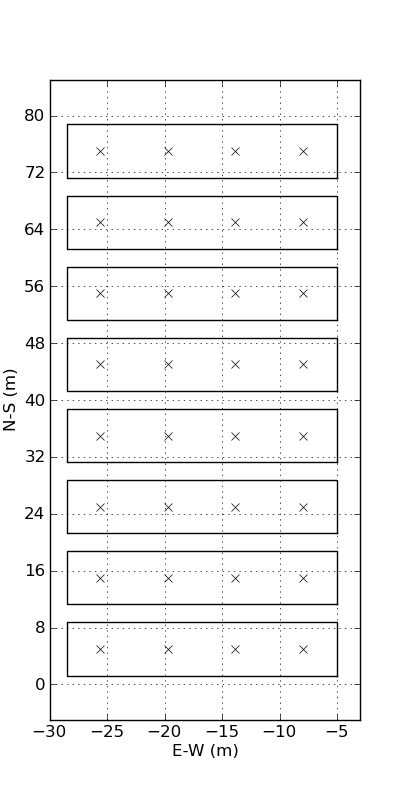
\includegraphics[scale=0.6]{graphics/layout.png}
    \label{fig:ant_layout}
    }
    \hspace{10pt}
    \subfloat[BEST-2 is a subset of eight cylinders in the north-south arm of the Croce del Nord.]{
    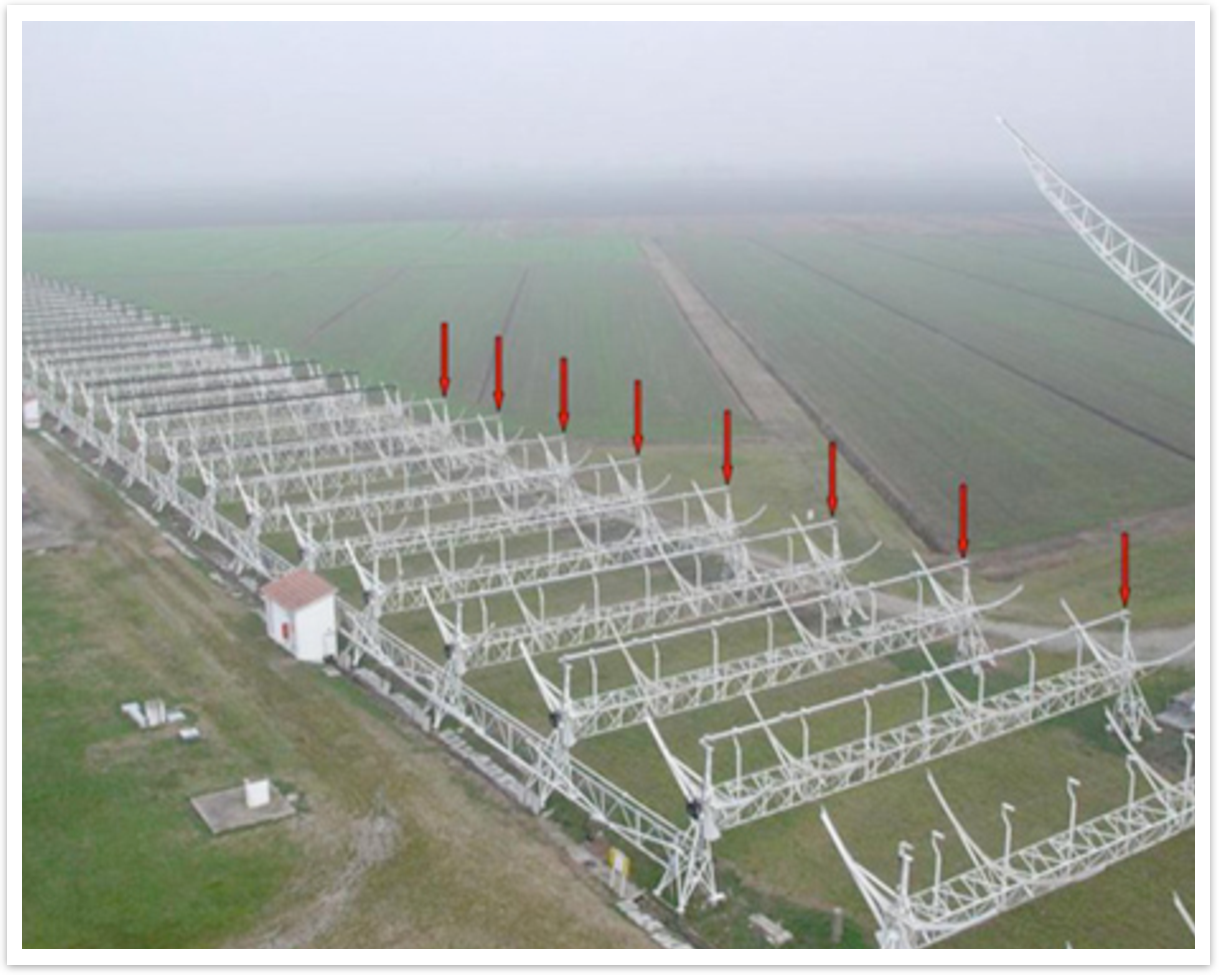
\includegraphics[scale=0.4]{graphics/best2.pdf}
    \label{fig:best2}
    }
    \caption{BEST-2 antenna geometry.}
    \label{fig:array_layout}
\end{figure}

\section{Instrument Design}
\label{instrument design}

An FX correlator and spatial FFT imager instrument have been built for BEST-2.
The hybrid design of our digital instruments make it possible to use both the correlator and imager concurrently.
Both instruments use the same digitization and channelization frontend.
This allow a streamlined process of calibrating the spatial FFT imager, reduces the amount of hardware and allows for simultaneous observation with both instruments.
The instrument has been implemented on ROACH boards which are a generic field programmable gate array (FPGA) board designed by CASPER for radio astronomy applications.
A ROACH consist of a XILINX Virtex 5 SX95T FPGA with interfaces to DRAM and QDR memory, high speed CX-4 connectors and a generic Z-DOK interface for connecting ADCs and various daughter boards, fig \ref{fig:roach}.
Additionally, the board has a PowerPC running BORPH, a variant of Debian Linux, which allows access to software registers and shared memory on the FPGA.
Firmware is designed using MATLAB Simulink which is extended with XILINX DSP blocks and CASPER's open source DSP blocks\footnote{https://casper.berkeley.edu/}.
Design specific DSP blocks and hardware interfaces have also created, design models and control software are available from our project repository\footnote{https://github.com/griffinfoster/medicina}.
Instrument design specifications are presented in table \ref{tbl:digital_specs}, further design detail is described in sections \ref{channelization}, \ref{correlator} and \ref{s-engine}.

\begin{figure}
    \centering
    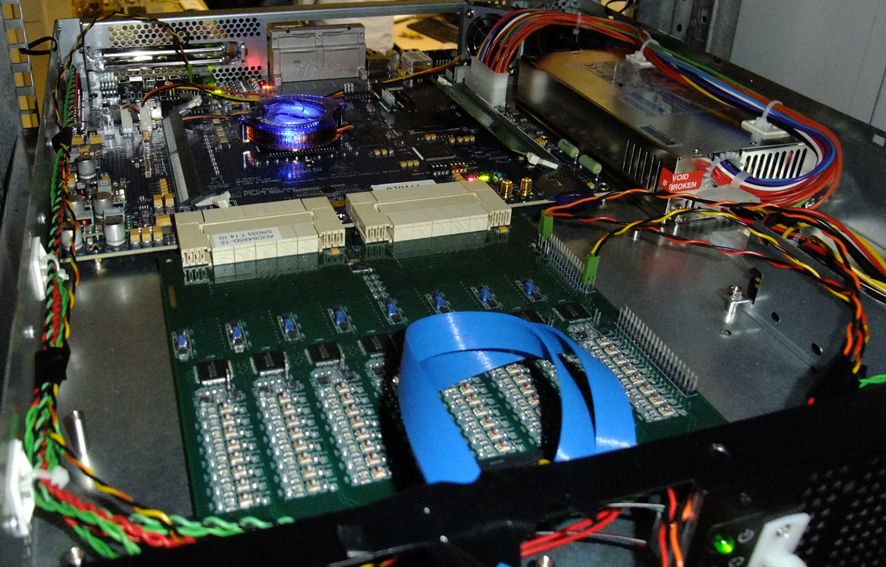
\includegraphics[scale=0.4]{graphics/roach_feng.png}
    \caption{The 'f-engine' ROACH board, a Virtex 5 SX95T FPGA board, with the 64 input ADC connected via two Z-DOK connectors.}
    \label{fig:roach}
\end{figure}

\begin{table}
\begin{center}
\begin{tabular}{| l | l | l |}
\hline
\multicolumn{3}{|c|}{Digital Backend Specifications}\\
\hline
Digitizer/Channelizer (F-Engine) & &\\
\hline
ADC Sampling Rate	& 40 			& MHz\\
ADC Sampling Precision	& 12 			& bit \\
Antenna-polarizations 	& 32 			& single pol \\
PFB 			& 4 tap FIR + 2048 point FFT	& Radix-2 Biplex Real FFT\\
Quantization 		& 4 			& bit\\
& & \\
\hline
FX Correlator (X-Engine) & &\\
\hline
Auto Correlations 	& 32 			& \\
Cross Correlations 	& 496 			& \\
Minimum Integration Length & 6.55 		& ms\\
Output 			& 10 GbE 		& SPEAD protocol\\
& & \\
\hline
Spatial FFT Imager (S-Engine) & &\\
\hline
2D FFT 			& 8 x 16 		& \\
Beams 			& 128 			& \\
Minimum Integration Length & 1 			& s\\
Output 			& 1 GbE 		& SPEAD protocol\\
Beamformer Output 	& 10 GbE 		& Up to 8 Beams\\
& & \\
\hline
\end{tabular}
\caption{A three ROACH design where the correlator and spatial FFT imager use the digitizer/channelizer interface.}
\label{tbl:digital_specs}
\end{center}
\end{table}

\subsection{Digitization and Channelization}
\label{channelization}

Signal digitization is performed using the Texas Instruments ADS5272 8 channel, 12 bit ADC.
The ADC board, developed by Rick Raffanti \footnote{https://casper.berkeley.edu/wiki/64ADCx64-12}, uses eight of these ADCs to channelize 64 streams at up to 65 Msps.
In our design only 32 signal streams are digitized at 40 Msps which covers the 16 MHz analogue band.
The ADC is clocked with a 160 MHz clock which is locked to a local maser source.
During the analogue stage the RF, centered at 408 MHz, has been mixed down to baseband.
Prior to digitization the last amplifier stage of the analogue chain has per signal adjustable gain useful for setting levels for ADC quantization.
This ADC is connected via a dual Z-DOK interface to an `F-Engine' ROACH which performs the channelization.
A block diagram of the design layout is shown in figure \ref{fig:feng_block}.

The ROACH board is clocked at four times the sample rate such that four signals are time division multiplexed onto a single stream.
Channelization is performed with a four tap Hann filter, 2048 point polyphase filterbank (PFB) to produce 1024 samples per real antenna stream.
The CASPER PFB has been modified to account for the signal multiplexing.
Each channel has a width of 19.5 kHz and the output of the FFT stage is a 36 bit complex number.
The narrow channel widths and PFB windowing allows for good frequency separation in the high RFI environment at the observatory.
After channelization the samples are quantized down to 8 bit complex.
An adjustable, per channel complex gain equalizer is used for amplitude and phase corrections before quantization.
Complex gain calibration is essential to proper spatial FFT imaging which must be applied before the spatial FFT.
The FX correlator is used to generate calibration coefficients which are applied back into the equalizers.
A selectable mux is available to skip the phase coefficients on the FX correlator data stream.
Post equalization, the data stream is split in two for specific reordering for the correlator and imager.
The correlator data stream is reordered to 128 time samples for a single antenna for a single frequency channel.
Followed by the next antenna and cycles back onto the next frequency channel.
The imager takes in one time sample of each antenna for a given frequency channel and cycles through 128 time samples before stepping to the next frequency channel.
After data reordering each stream is sent over high speed XAUI at a rate of 5.12 Gbps to the correlator and imaging boards.
The FPGA resource usage is listed in table \ref{tbl:feng_resource}.
There is sufficient resources to include additional features in the `F-Engine', i.e. finer channelization, increase in antennas, increase in bandwidth.

\begin{table}
\begin{center}
\begin{tabular}{| l | l | l |}
\hline
\multicolumn{3}{|c|}{F-Engine ROACH Resource Utilization (Virtex 5 SX95T)}\\
\hline
ADC Clock 		& 40 MHz \\
System Clock 		& 160 MHz 	& Demux:4 \\
Slice Registers 	& 30217 / 58880 & $51\%$\\
Look Up Tables 		& 24319 / 58880 & $41\%$\\
BRAM (36kb) 		& 205 / 244 	& $84\%$\\
DSP48e (Multipliers) 	& 185 / 640 	& $28\%$\\
CX-4 Interface 		& 2 / 4 	& 5.12 Gbps XAUI\\
QDR Memory 		& 2 / 2 	& Cornerturn\\
\hline
\end{tabular}
\caption{DSP implementation of the f-engine ROACH board}
\label{tbl:feng_resource}
\end{center}
\end{table}

\begin{figure}
    \centering
    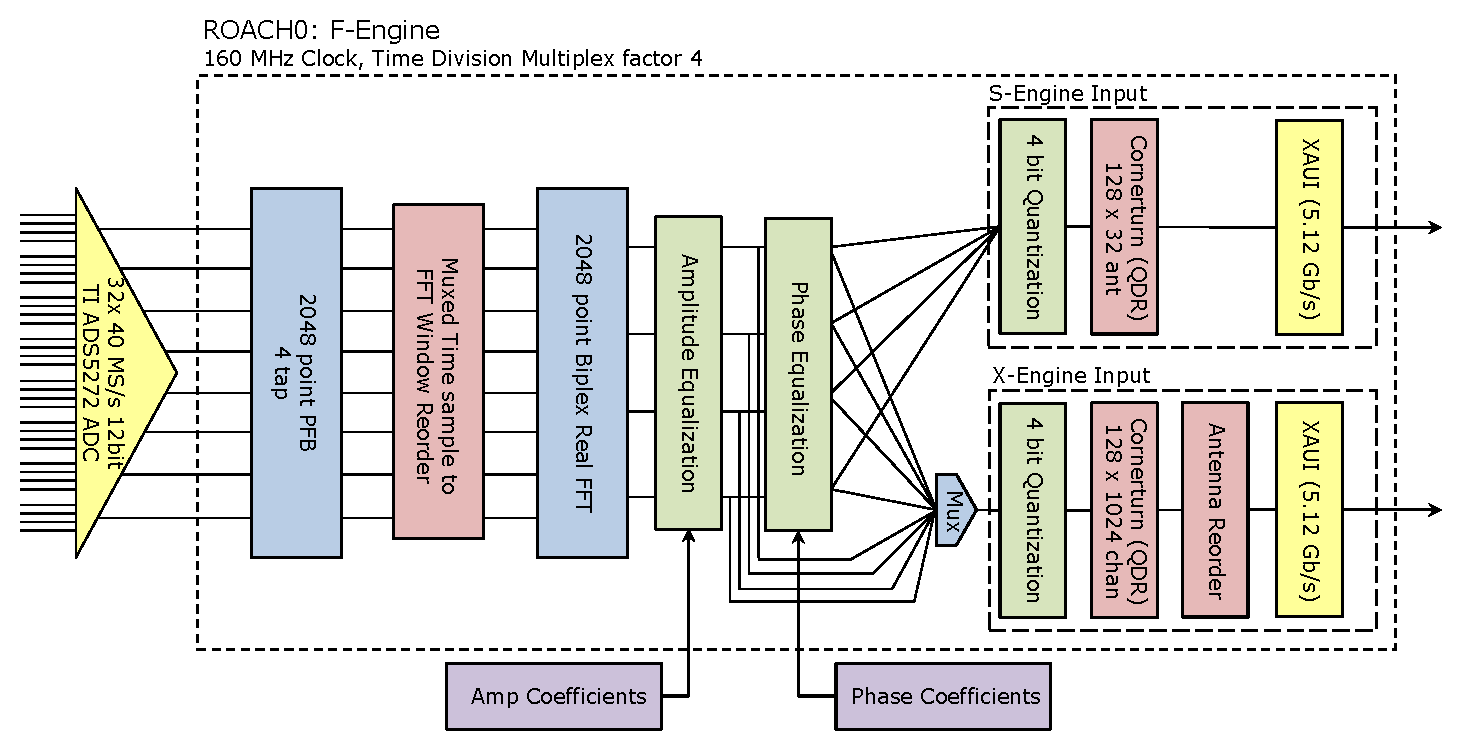
\includegraphics[scale=0.6]{graphics/crop_fengine_block.pdf}
    \caption{During observations amplitude and phase coefficients are applied to scale the power for the 4 bit correlation and apply phase corrections for the spatial FFT.}
    \label{fig:feng_block}
\end{figure}

\subsection{FX Correlator}
\label{correlator}

An FX correlator design is a standard design for large bandwidth and many antenna arrays.
The F component represents the frequency channelization, and the X is a complex multiply and accumulate (CMAC).
An overview of the architecture is presented in \citep{casper}.
Architecture efficiency goes as $O( M \textrm{log} M) + O( N^2)$ where $M$ is the number of FFT frequency channels and $N$ is the number of antenna-polarizations.
The core component to the X stage of the FX correlator is the complex multiplication of all pairs of independent signals for each frequency channel.
A pipelined x-engine, based on the general CASPER block originally designed by Lynn Urry\citep{fxcorrelator}, is used for multiplier efficiency.
The pipeline design is constructed out of $M/2$ `taps' where the $i^{th}$ tap computes the correlation between antennas $A_j$ and $A_{j+i}$ for every antenna $A_j$ of $M$ total antennas.
To maximize the multiplier usage a loopback is added to use every $i^{th}$ tap to compute the correlation of antennas $A_j$ and $A_{M/2+j+i}$, fig. \ref{fig:xeng_pipe}.
Each tap accumulates for $N$ time samples to reduce the output data rate.

\begin{figure}
    \centering
    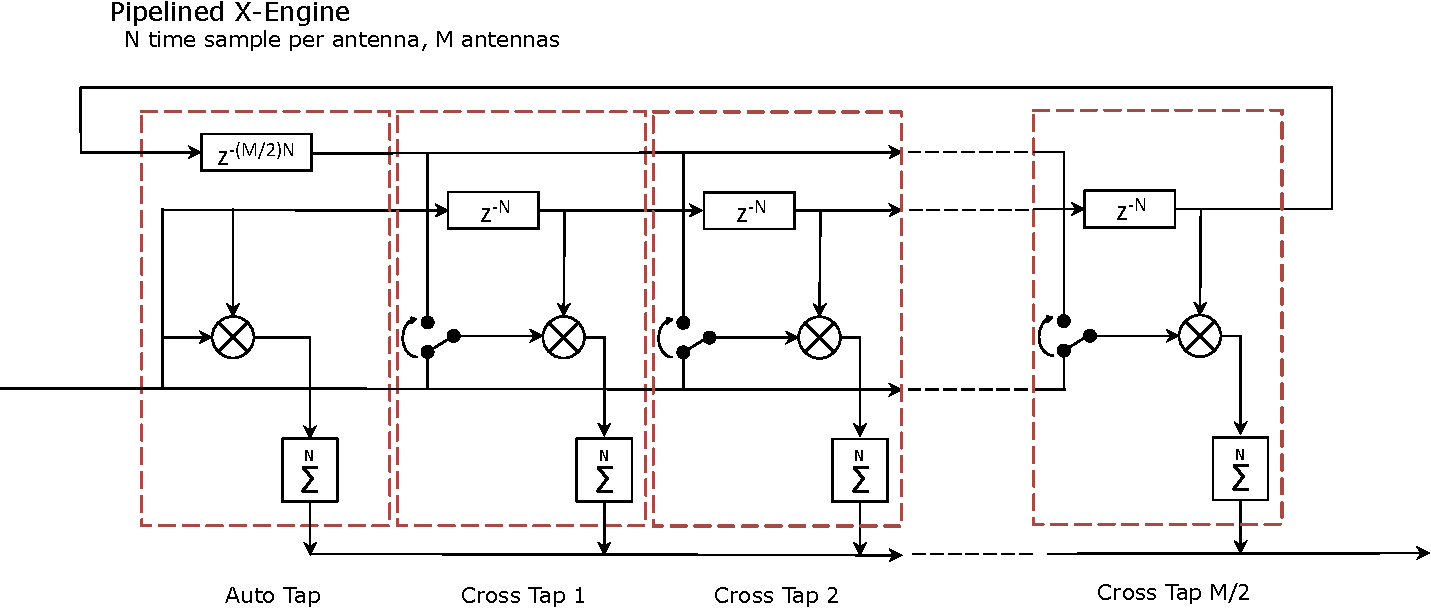
\includegraphics[scale=0.6]{graphics/crop_pipelined_xeng.pdf}
    \caption{The input is ordered as $N$ time samples per antenna per frequency channel. An accumulation stage after the complex multiply reduces the data rate of each tap. Outputs are multiplexed onto the same output using a valid signal.}
    \label{fig:xeng_pipe}
\end{figure}

An asynchronous architecture is used between the f-enigne and x-engine boards.
The x-engine board has been clocked to 200 MHz, well above the 160 MHz f-engine board, this assures the x-engine board will never have input buffer overflows during the windowing stage.
The XAUI interboard connection is a streaming interface which guarantees the same output order as input order but with variable latency.
In rare cases the XAUI interface can drop 64 bit words during the streaming, this requires an initial stage to track the number of words received between headers.
In case of missing words the entire payload is dropped and counters reset for the next header.
A correlation is only performed on a per channel basis.
The channelized band can be split up into portions and processed in parallel across multiple x-engines.
This allows a larger bandwidth to be processed at the cost of increased logic and multiplier resource utilization.
We currently under utilize the available resources on the FPGA, table \ref{tbl:xeng_resource}.
For this design two pipelined x-engines are used which each processes half of the band, figure \ref{fig:xeng_block}.

The x-engine design requires a continuous stream of data for 128 samples of all antennas for a single frequency channel.
Prior to the x-engine samples are buffered up into windows to guarantee valid data during a cycle of the x-engine.
For reasons related to the design the 32 single polarization signals are treated as 16 dual polarization signals.
This causes a small number of redundant baseline correlations and a conjugation effect which is corrected in post processing.
During the x-engine stage an initial accumulation of 128 sample is performed after the complex multiply to reduce the output rate to roughly the input rate.
This limits the minimum integration time to 6.55 ms.
In addition to the standard CASPER pipelined x-engine design an optimized version has been tested.
This new optimized design efficiently uses the full bit width of the Xilinx DSP48 multipliers to reduce the total multiplier usage by a 75\%.
A description of this optimized design is in preparation.

A vector accumulator using the on board QDR memory is used for longer integration lengths.
This second accumulator is software controlled with integration lengths ranging from milliseconds to minutes.
A completed integration is sent to a receive computer over a 10 GbE connection.
Integrations are split up based on the SPEAD protocol\footnote{https://github.com/ska-sa/PySPEAD} and transmitted as UDP packets.

\begin{table}
\begin{center}
\begin{tabular}{| l | l | l |}
\hline
\multicolumn{3}{|c|}{X-Engine ROACH Resource Utilization (Virtex 5 SX95T)}\\
\hline
System Clock & 200 MHz \\
Slice Registers & 28494 / 58880 & $48\%$\\
Look Up Tables & 25349 / 58880 & $43\%$\\
BRAM (36kb) & 88 / 244 & $36\%$\\
DSP48e (Multipliers) & 288 / 640 & $45\%$\\
CX-4 Interface & 1 / 4 & 5.12 Gbps XAUI\\
QDR Memory & 2 / 2 & Vector Accumulator\\
\hline
\end{tabular}
\caption{DSP implementation of the x-engine ROACH board.}
\label{tbl:xeng_resource}
\end{center}
\end{table}

\begin{figure}
    \centering
    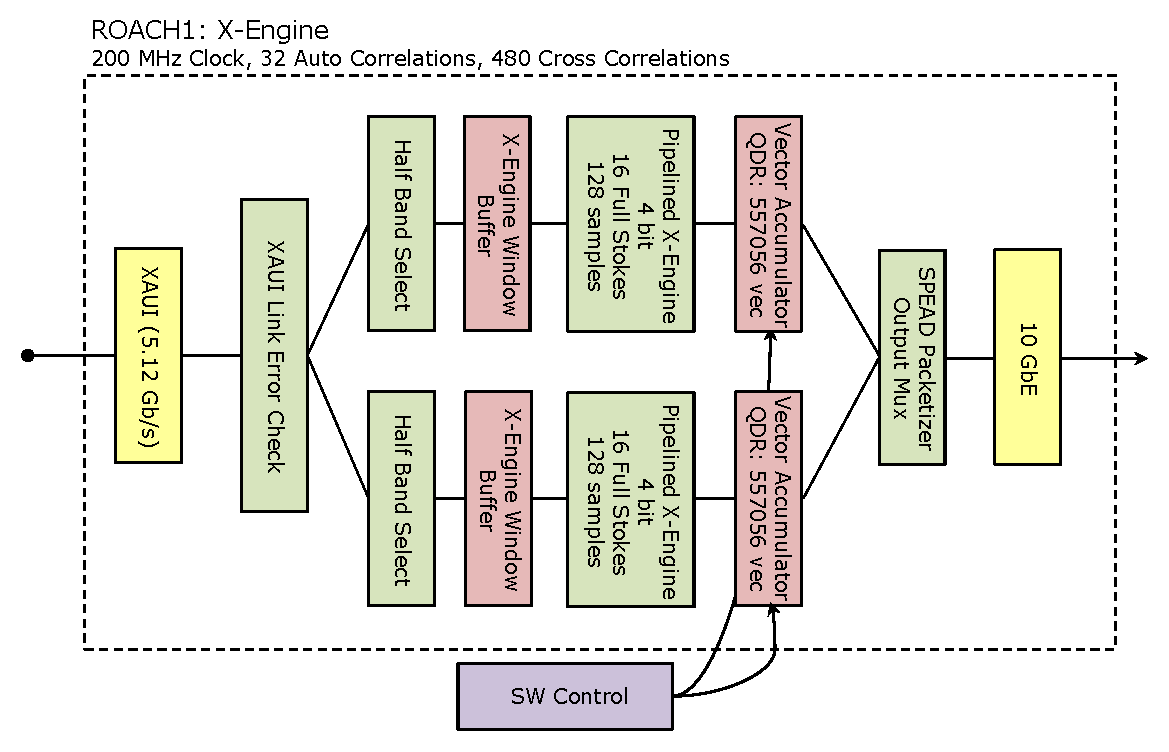
\includegraphics[scale=0.6]{graphics/crop_xengine_block.pdf}
    \caption{Two parallel pipelined x-engines are used, each processes half of the band.}
    \label{fig:xeng_block}
\end{figure}

\subsection{Spatial FFT}
\label{s-engine}
 
When $N$ receiving elements in an antenna array are placed on a regularly spaced grid, a well known method for producing a complete set of orthogonal beams on the sky is the spatial fast Fourier transform \citep{fastbeamforming}.
Such a beamforming implementation will generate $N$ beams on the sky, with a computational cost of $O(N\log{N})$. For large arrays, where many beams are desired, this can be a significant computational saving, with the alternative, so-called \emph{DFT beamforming}, requiring $O(N)$ operations per synthesized beam.
To date, the largest such astronomical implementation of such a spatial fast Fourier transform beamformer is the 64 element dish array constructed in 1994 at Waseda University, Japan \citep{2dfft}.

More recently, spatial FFT based processing has been revisited in the literature with an emphasis on the correlation matrix, rather than the collection of beams, as the mathematical object of interest \citep{fftt} \citep{omniscope}.
In the method outlined by Tegmark \& Zaldarriaga, zero padding is applied to the matrix of antenna signals before the spatial FFT is performed, and as such, the complete set of visibilities for all unique baselines in the array can be obtained, post integration, by inverse Fourier transform.
Conversely, in the image plane, the zero-padding required by the prescribed algorithm results in the generation of $~2^{m}N$ beams on the sky and is dependent on the number of dimensions, $m$, in the antenna array.
Regardless of potential downstream visibility domain processing, this oversampling of the sky by a factor $2^{m}$ has the benefit of increasing the instantaneous uniformity of sky coverage by synthesized beams, which somewhat alleviates the limitations associated with the inability to steer multiple beams independently.

%A spatial FFT imager is a novel instrument which takes advantage of the baseline redundancy in a regularly gridded array to reduce the correlator cost of an FX design $O(n^2)$ to a FFT cost of $O(n \log{n})$.
%Correlation of all antenna pairs in a regularly gridded array makes redundant measurements for many of the baselines.
In the BEST-2 backend described here, the requirements on the spatial FFT processor were multifold.
Firstly, the system should be capable of generating images on an $O(\mathrm{second})$ timescale, by the method described by \citep{fftt}.
Further, the system should be capable of passing formed beams at full bandwidth, i.e. without any accumulation, to downstream time domain processing systems such as the real-time pulsar dedispersion engine \citep{dedispersion}. 

This redundancy for the BEST-2 array is show in figure \ref{fig:redbl}.
Instead of making individual correlations of the same baseline as in an FX correlator the correlation of the average of each baseline can be computed.
This optimization relies on the assumption that each redundant baseline measurement is indeed identical.
Thus any calibration to the complex gains must be applied before the spatial FFT.

\begin{figure}
    \centering
    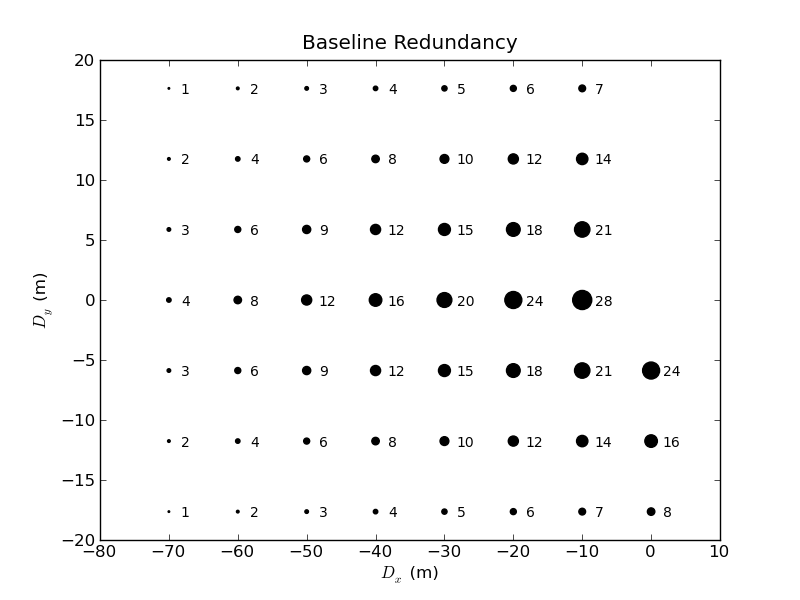
\includegraphics[scale=0.6]{graphics/redbl.png}
    \caption{A 4 by 8 regularly gridded array has 53 unique baselines, 480 cross correlations are performed. The number of redundant baseline measurements is shown as the color and size of each circle.}
    \label{fig:redbl}
\end{figure}

Though the X-Engine and S-Engine use the same F-Engine each requires a unique data windowing order.
For the S-Engine a window is made up of N antennas by M time samples for a given frequency channel.
A similar XAUI interface and windowing scheme is used as in the X-Engine which buffers up windows of valid data to stream into the spatial transform.
The 2D spatial transform is performed using an 8 point FFT followed by a cornerturn and 16 point FFT.
A block diagram of the design layout is shown in figure \ref{fig:seng_block}.
The BEST-2 array is a grid of 4 by 8 antennas, the data is zero padded before input into the 8 by 16 point spatial transform.
A 4 by 8 point spatial transform will only produce gain information for each spatial position, which can be interpreted as an array of beamformers covering the field of view.
This zero padding is necessary to produce both the gain and phase information of each spatial position which is an effective baseline.
Each effective baseline is an average of all possible baselines with the same spatial dimensions.
The four fold increase is the number of outputs from the spatial transform by double padding introduces a number of redundant calculations.
The spatial transform produces 128 outputs.
There are only 53 unique baselines in a 4 by 8 grid.
The datarate out of the S-Engine is reduced by a two stage vector accumulator.
A fixed 128 sample vector accumulator reduces the output of the second stage FFT so that the 1024 channels of the 128 computed spatial components can be multiplexed onto one line and accumulated in a software controllable QDR vector accumulator.
Accumulations are sent out over the 1 GbE PowerPC interface using the a SPEAD UDP packet format.
Individual beams can be selected out before accumulation and sent over 10 GbE in a LOFAR beam packet format which will be used for future pulsar processing.

\begin{figure}
    \centering
    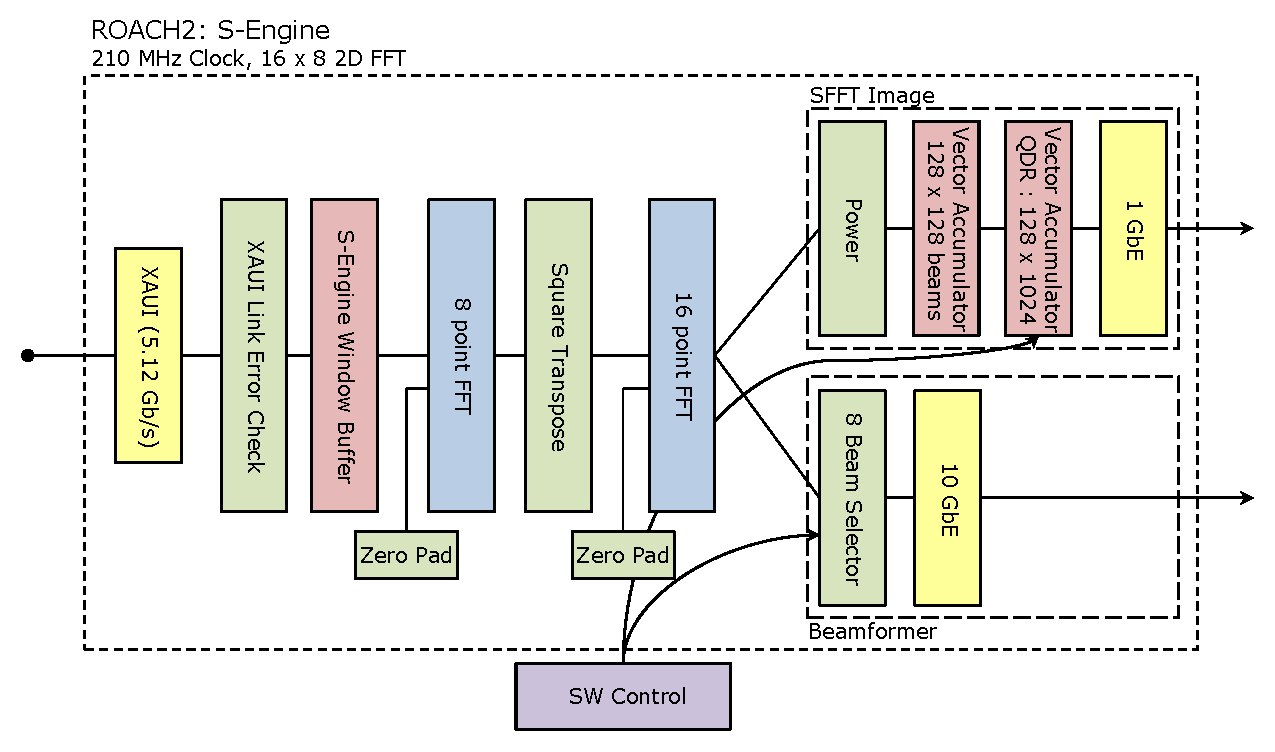
\includegraphics[scale=0.6]{graphics/crop_sengine_block.pdf}
    \caption{During the two stage spatial FFT the streams are zero padded to provide phase information of each baseline.}
    \label{fig:seng_block}
\end{figure}

\section{Deployment and Initial Observations}
\label{observations}

Instrumentation was installed and tested over a two week period in March 2012.
During that time a number of test signals were used to check the system status.
Various bright radio sources were observed once the analogue and digital systems were checked out.
Since the Northern Cross is a transiting array there is a limited period of time each day in which a source is in the primary beam.
Bright sources such as Cygnus A, Cassiopeia A and Taurus A along with a number of 3C sources were observed along with multiple constant declination 24 hour cycles.

Raw data from the correlator and imager was recorded to HDF5 files using a SPEAD protocol receive script.
A suite of python scripts have been written to interface and manipulate the data in this pre-calibration stage.
A python FITS-IDI package has been written to convert HDF5 files into the standard FITS format which can be read by AIPS and CASA\footnote{https://github.com/telegraphic/pyfitsidi}.
This allows for conversion to the Measurement Set format which most packages can interface with.

\subsection{FX Correlator Imaging}
\label{fx_results}

During observations no phase tracking is applied to the antennas.
The integration time is sufficiently short that this does not effect the phase.
This allows the array to be phase tracked to any position in post processing.
Before conversion to measurement sets a phase center is chosen and a phase correction is added to each integration.
We are limited to a fixed observation length per day for a given source.
The UV coverage is essentially the same for any observation, with some variation due to pointing declination. 

The East-West full width half max (FWHM) beam size of an individual element is $\approx11.25^{\circ}$ which translates to a 45 minute `transit time' for a source, as seen in the measured primary beam, figure \ref{fig:best2_pb}.
For the the bright A class sources this time can be extended since they remain the dominating source well after crossing the FWHM.
Observations of 80-90 minutes are possible which gives an small improvement in uv coverage at the cost of properly accounting for the amplitude modulation due to the primary beam.
This warrants a small sensitivity benefit for a large calibration cost.
Most images are created using data within a few minutes of the source transit time.
The high sidelobes in the primary beam, figure \ref{fig:best2_pb}, cause the bright class A sources to dominate even when they are far from the field of view and makes it difficult to perform calibration and imaging near these sources.

\begin{figure}
    \centering
    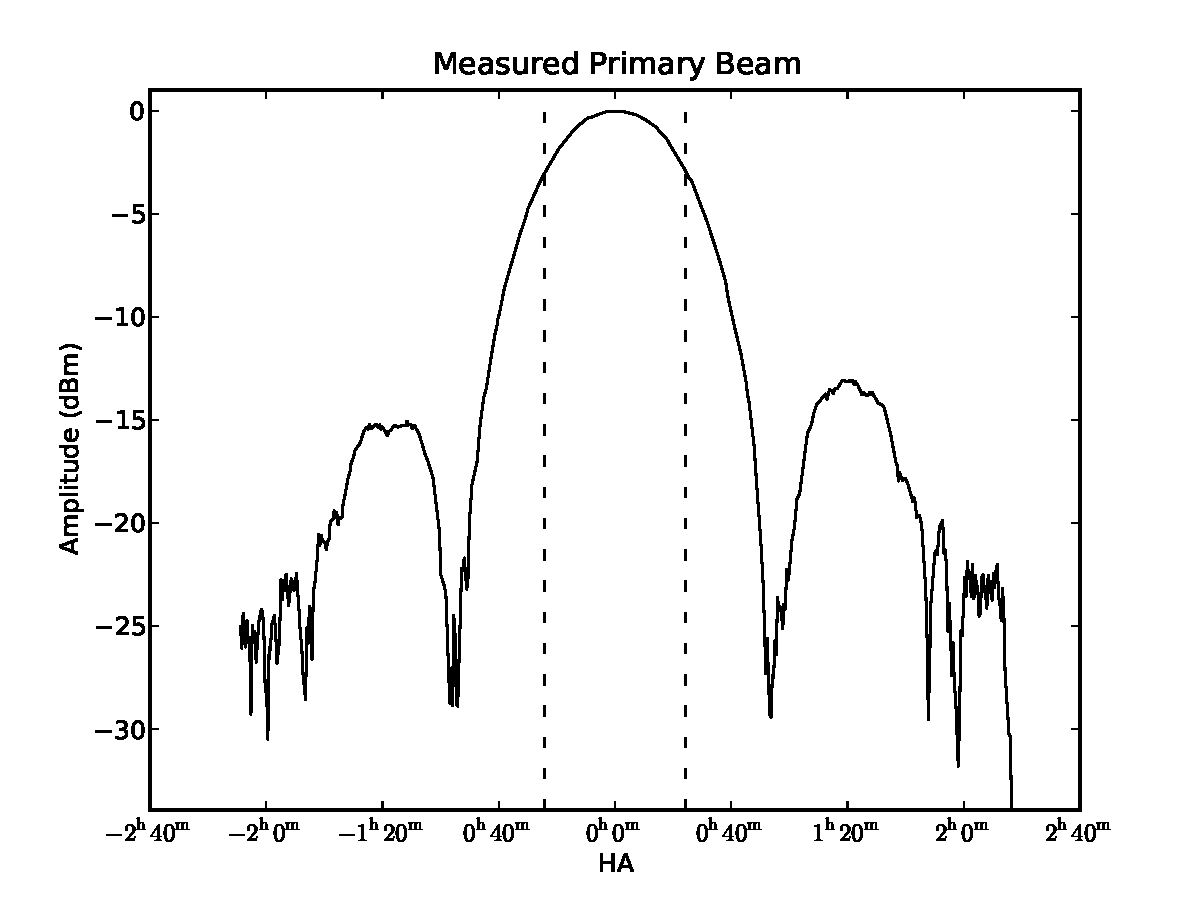
\includegraphics[scale=0.6]{{graphics/pb/best2_3_20_primary_beam}.pdf}
    \caption{A measured east-west primary beam based on the correlation between antennas 1N-6-1 and 1N-1-3, which are representative of typical antennas, based on a Cassiopeia A transit. The dashed lines indicate the FWHM points. The antennas should have a sinc response to a point source, as expected the first sidelobes are -15 dB down from the peak.}
    \label{fig:best2_pb}
\end{figure}

%calibration/flux scale
A transiting array provides a unique challenge of gain calibration since a source's apparent gain will change as it transits the primary beam.
To account for this a two stage gain calibration method is used.
Phase calibration and setting the flux scale is accomplished using Cassiopeia A and Cygnus A observations as point source sky models set to their 3C flux levels and known spectral indices.
Since these sources are very bright, only a few seconds at transit is needed produce a high SNR dataset to use for calibration.
Over this period the primary beam can be approximated as flat.
A time independent complex gain is derived for a coarse calibration.
After applying the gain corrections an observation will be set to a flux scale relative to the flux of the calibration source.
Each individual source is then self calibrated in MeqTrees\citep{meqtrees} based on a local sky model taken from the 3C catalog.
This stage is calibrated on short time intervals to account for amplitude changes from the primary beam.

%psf/dirty/clean
%dynamic range/noise/SEFD
An effect of the density of the antenna layout is a low point spread function(PSF) to field of view ratio (spatial fidelity), thus images tend to contain at most a few spatial separate point sources.
The grid layout of the BEST-2 array produces strong sidelobes and grating lobes in the PSF as seen in figure \ref{fig:fx_tau_psf}.
Observations of bright point sources produces calibrated dirty images in which the PSF is clearly visible, fig. \ref{fig:fx_tau_dirty}.
After cleaning we measure the residual noise to be around 2 Jy over a number of two minute snapshot observations, table \ref{tbl:src_flux}.
Imaging using longer source transit times has shown the noise floor to decrease at the expected rate.
The various stages of imaging an calibration for the source Taurus A is shown in figure \ref{fig:fx_tau}.
Further images and analysis of the data quality are followed in section \ref{sfft_results}.

%image: raw,psf,dirty,clean
\begin{figure}
    \centering

    \subfloat[Uncalibrated image of Taurus A.]{
    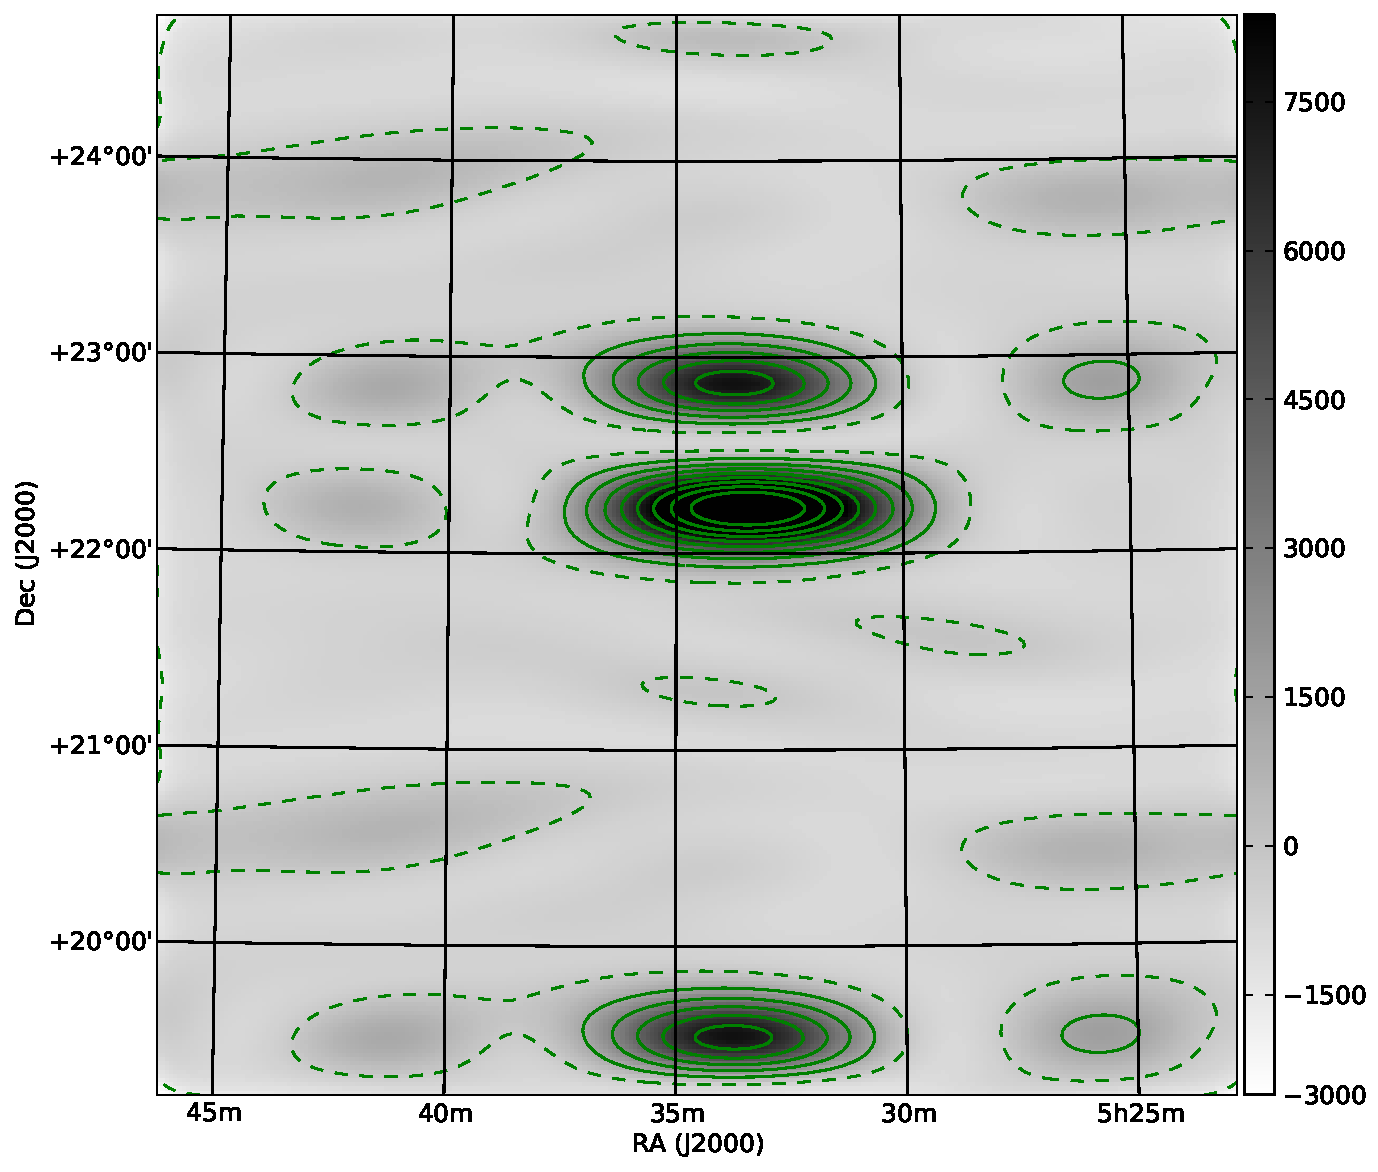
\includegraphics[scale=0.3]{{graphics/fx/corr.2455996.22803.tau.s.ms.DATA.channel.1ch}.pdf}
    \label{fig:fx_tau_data}
    }
    \hspace{10pt}
    \subfloat[Point spread function. The high, regular sidelobes are an effect of the regularly gridded array.]{
    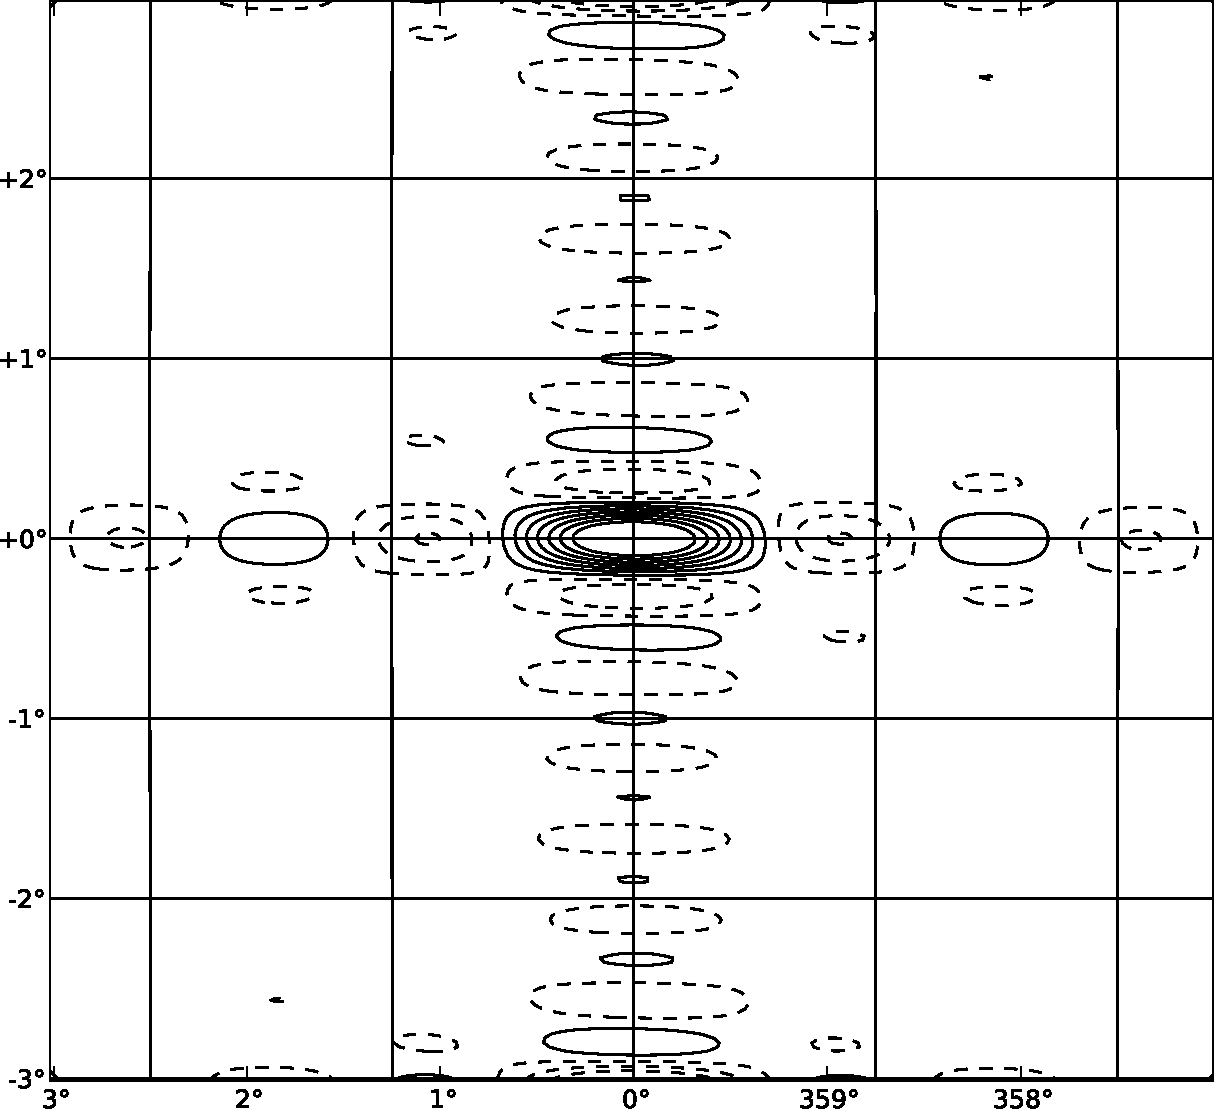
\includegraphics[scale=0.3]{{graphics/img.2455999.21403.tau.cal.s.ms.psf.channel.1ch.mod.crop}.pdf}
    \label{fig:fx_tau_psf}
    }
    
    \subfloat[Dirty image formed, using natural weighting, after applying complex gain solutions. The structure from the PSF is clearly visible. The dynamic range of this image is $\sim150$.]{
    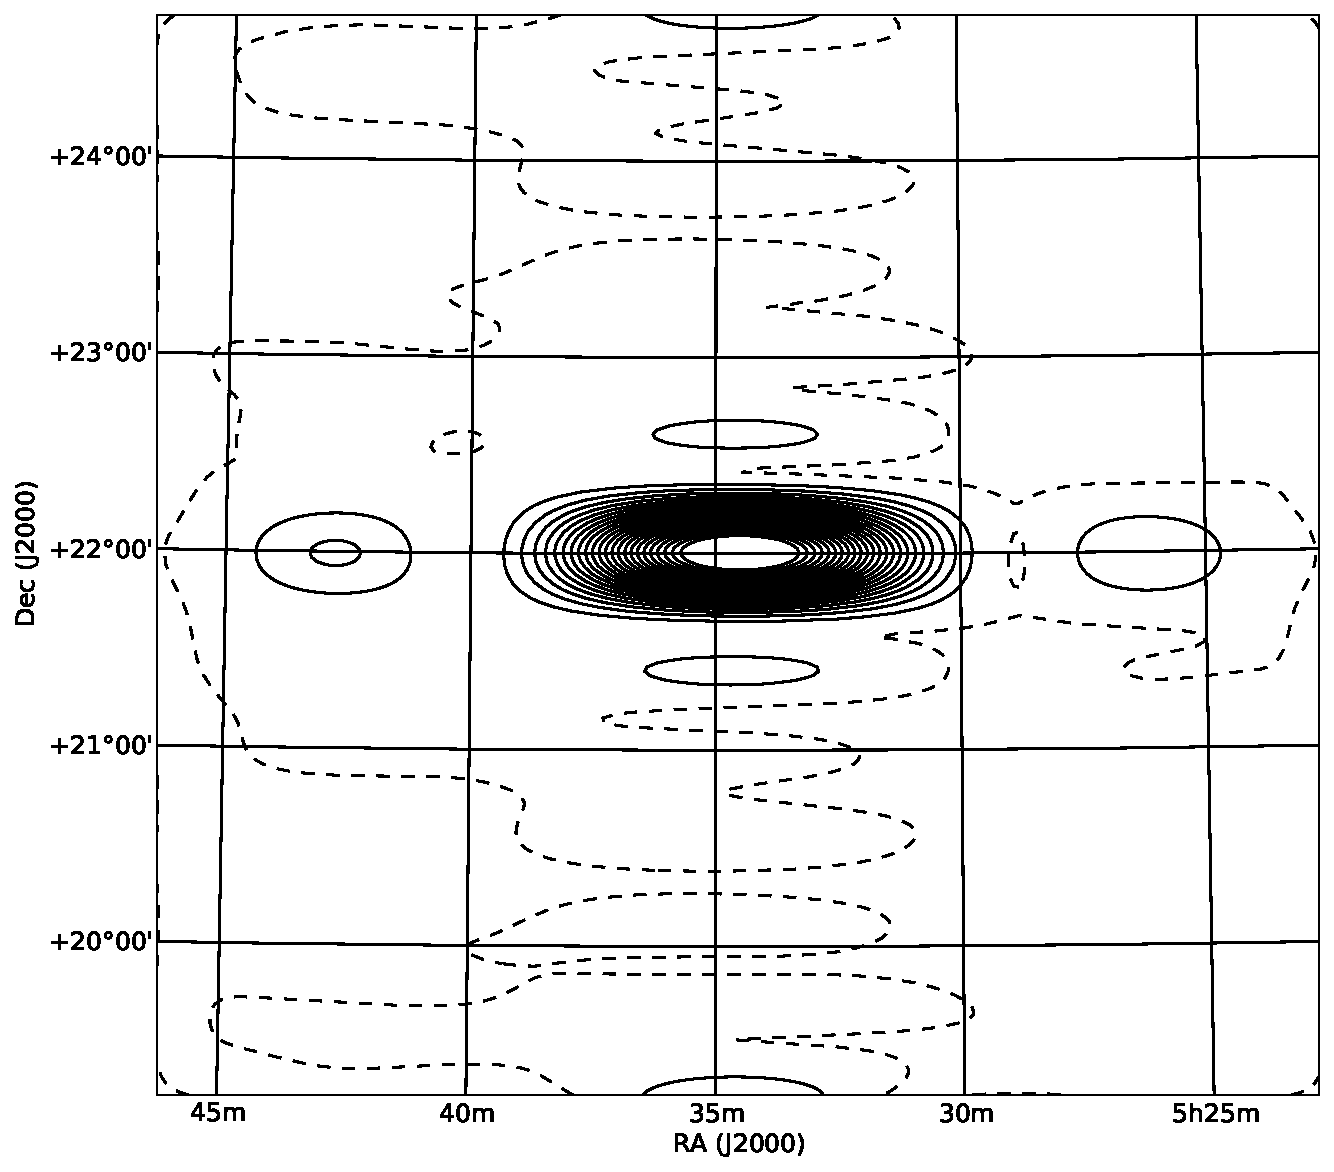
\includegraphics[scale=0.3]{{graphics/fx/corr.2455996.22803.tau.s.ms.CORRECTED_DATA.channel.1ch}.pdf}
    \label{fig:fx_tau_dirty}
    }
    \hspace{10pt}
    \subfloat[Cleaned image of the field, Taurus A is the dominating point source with a peak of 730 Jy, the image have a dynamic range of $\sim350$.]{
    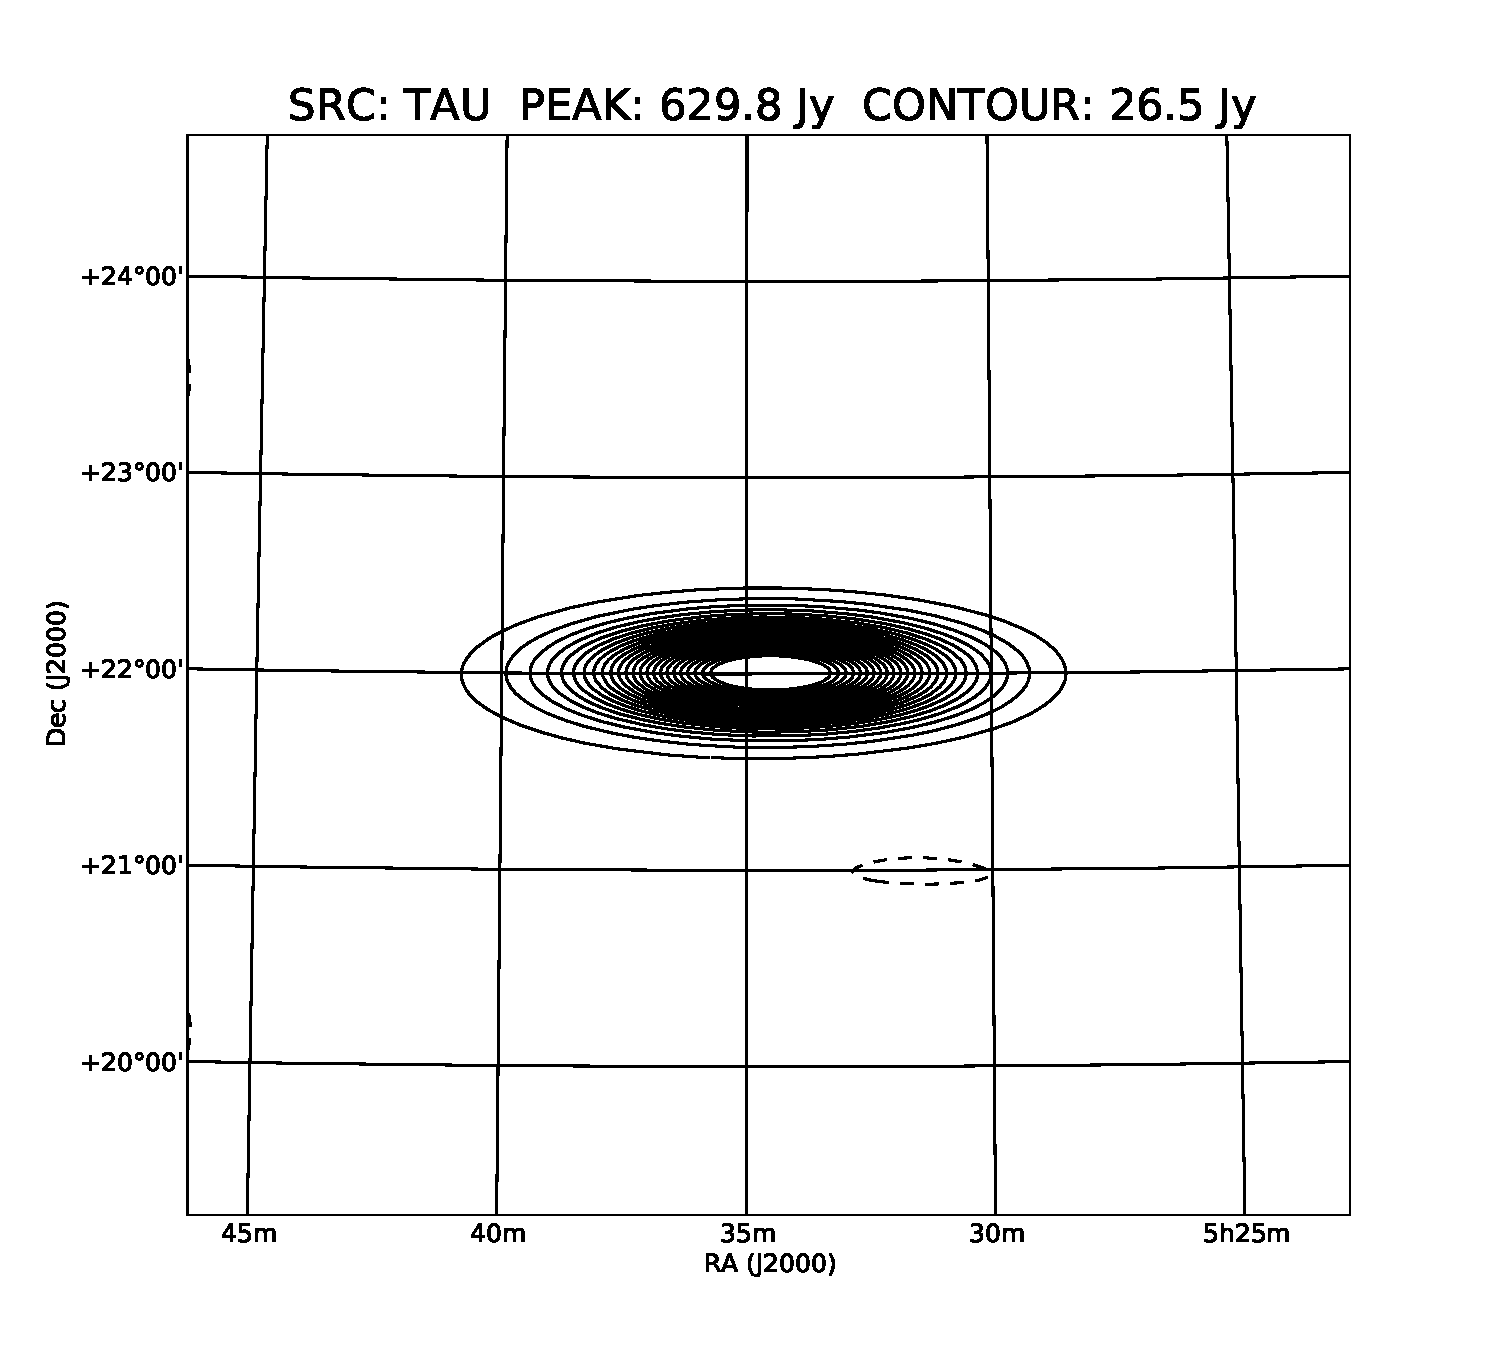
\includegraphics[scale=0.3]{{graphics/fx/corr.2455996.22803.tau.s.ms.CORRECTED_DATA.channel.1ch.restored}.pdf}
    \label{fig:fx_tau_clean}
    }
    
    \caption{Images and PSF formed from an FX correlator two minute snapshot observation of Taurus A.
    }
    \label{fig:fx_tau}
\end{figure}

%solar observation
\subsubsection{Solar Observation during Highly Active Period}

During calibration observations of Cassiopeia A a second source was found in the field.
The second source had approximately the same peak flux as Cassiopeia A and initially though to be a problem in the observation.
But it was shown to appear in multiple observations of the field and the source appeared to change position each day.
It has been determined that this second source was the Sun.
At the time of our observations, March 2012, the Sun was at a similar sidereal time as Cassiopeia A.
Also, in that time the Sun was undergoing a very active period which maybe one of the reasons we observed it at with a particularly strong flux.
Even though the Sun was at a declination of approximately $-4^{\circ}$, over $60^{\circ}$ way from Cassiopeia A, the source appears in the same field.
A combination of high primary beam sidelobes and an active solar period led to the sun being detected $62^{\circ}$ away from it's actual position.
The sun is approximately a half a degree in size, the longest north-south baseline is on the order of the same size and we begin to resolve the sun in that direction.
Figures \ref{fig:fx_cas_nosun} and \ref{fig:fx_cas_sun} show the Cassiopeia A field separated by 10 days, in that time the sun has moved well into the center of the field.
This made using Cassiopeia A as a calibration source not possible during our initial observations.

%image: cas, cas+sun
\begin{figure}
    \centering

    \subfloat[Observation of the Cassiopeia A field on Julian Date 2455985, the flux has been fixed to 5600 Jy with a dynamic range of $\sim900$. The structure on the edge of the image are likely from the sun beginning to come into the field of view.]{
    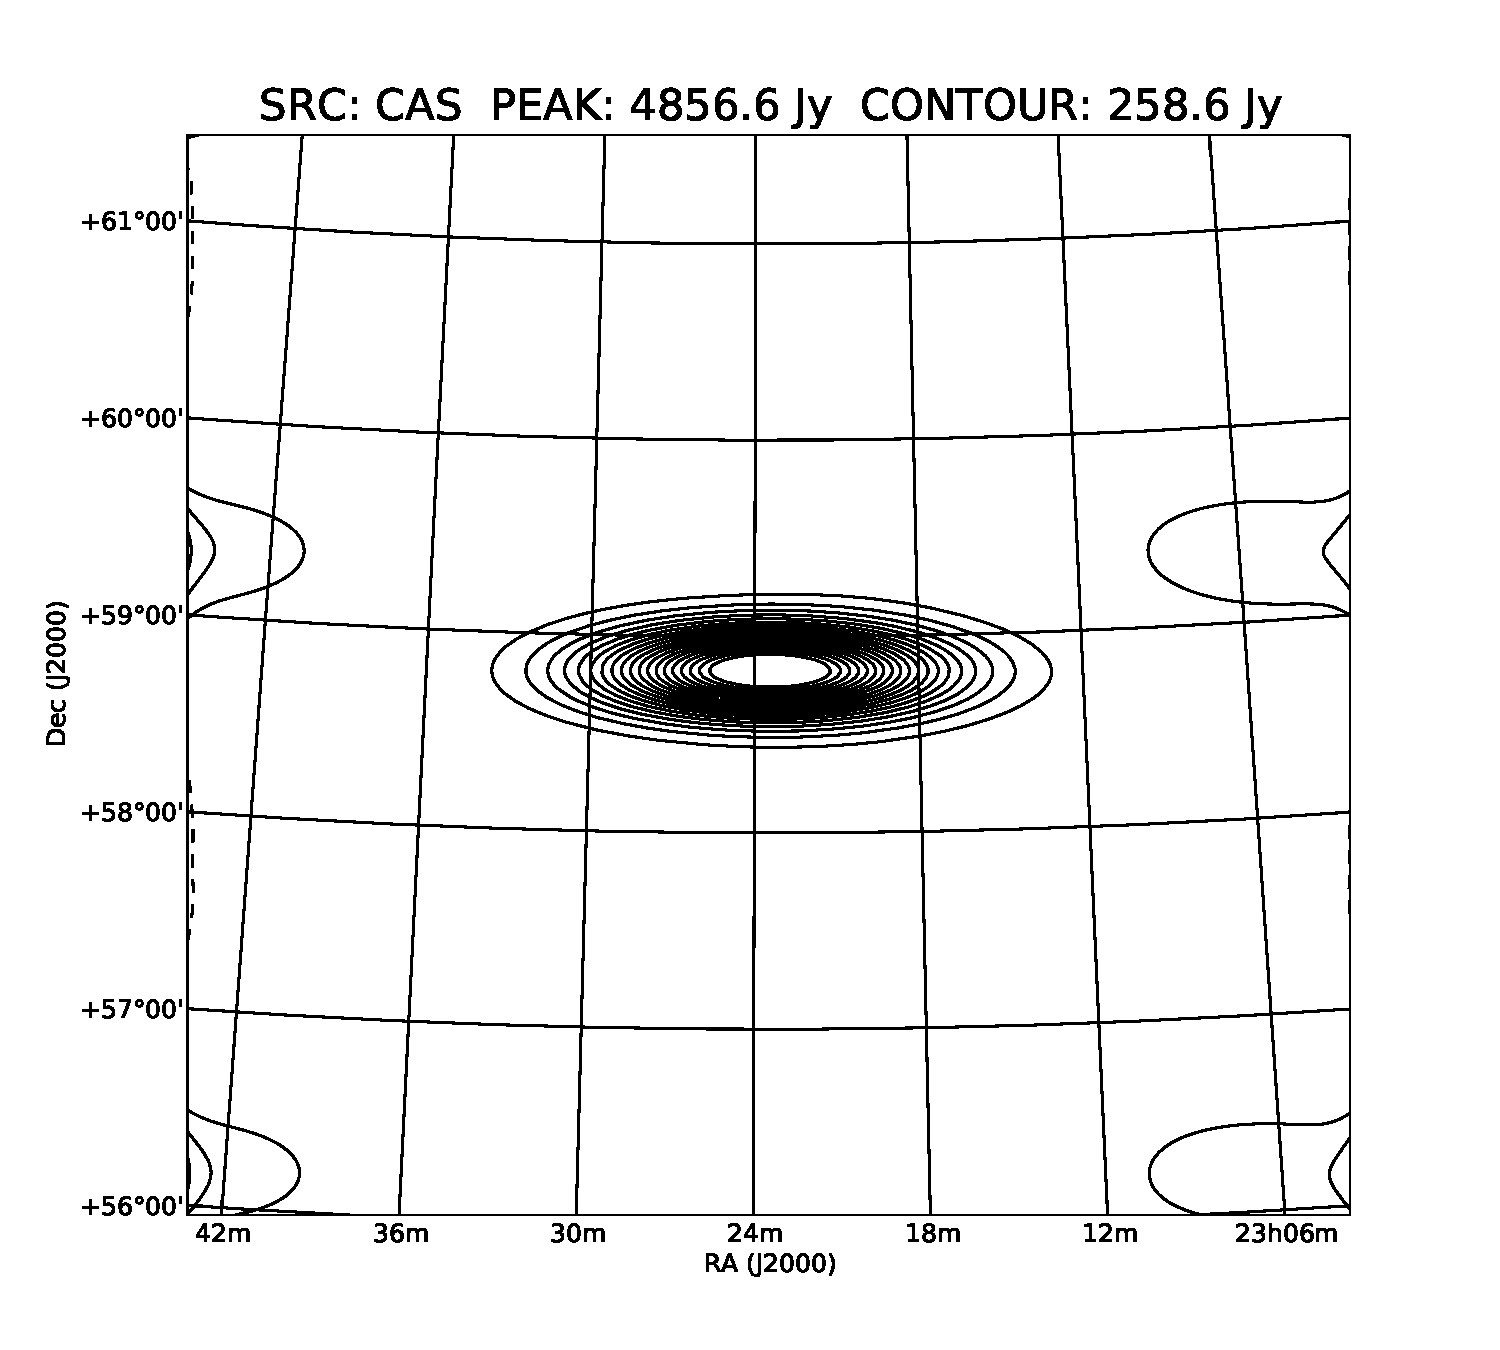
\includegraphics[scale=0.3]{{graphics/fx/corr.2455985.00383.cas.s.ms.CORRECTED_DATA.channel.1ch.restored}.pdf}
    \label{fig:fx_cas_nosun}
    }
    \hspace{10pt}
    \subfloat[Observation of the same field ten days later on Julian Date 2455996.
    The Sun is slightly resolved in the North-South direction.
    The Sun is at declination $-4^{\circ}$, about $62^{\circ}$ from the field of view but is within one of the primary beam sidelobes and has an apparent declination position at $58^{\circ}$.
    Using the same flux scale from the previous Cassiopeia A observation the Sun is measured to have a flux of 6000 Jy.
    Though, the Sun is being observed through a sidelobe this value is attenuated compared to the actual value.]{
    \includegraphics[scale=0.3]{{graphics/fx/corr.2455995.97200.cas.s.g.ms.CORRECTED_DATA.channel.1ch.restored}.pdf}
    \label{fig:fx_cas_sun}
    }
    
    \label{fig:fx_cas}
    \caption{Images of the Cassiopeia A field at different Julian dates show the Sun appearing in a primary beam sidelobe.
    }
\end{figure}

%weighting
\subsubsection{Weighting for a Regularly Gridded Array}

As noted, the regular gridded array produces many highly redundant baselines, fig. \ref{fig:fx_tau_psf}.
When forming the dirty image the choice of weighting greatly effects the outcome of the image.
In the highly redundant array case of BEST-2 the effects of using uniform versus natural weighting can be seen in fig. \ref{fig:fx_weighting}.
The uniform weighting scheme significantly reduces the sensitivity the image for a small improvement in spatial resolution.
We have used a natural weighting scheme through out to produce images.
It is worth noting that the baselines produced by the spatial FFT instrument have an inherent `natural' weighting scheme since all redundant baselines are effectively summed together into a single baseline.
To change the weighting of the spatial FFT baselines reweighting factors must be added to the data based on how redundant each baseline is.

%image: natural,uniform
\begin{figure}
    \centering

    \subfloat[Dirty image with natural weighting of the point source Taurus A.]{
    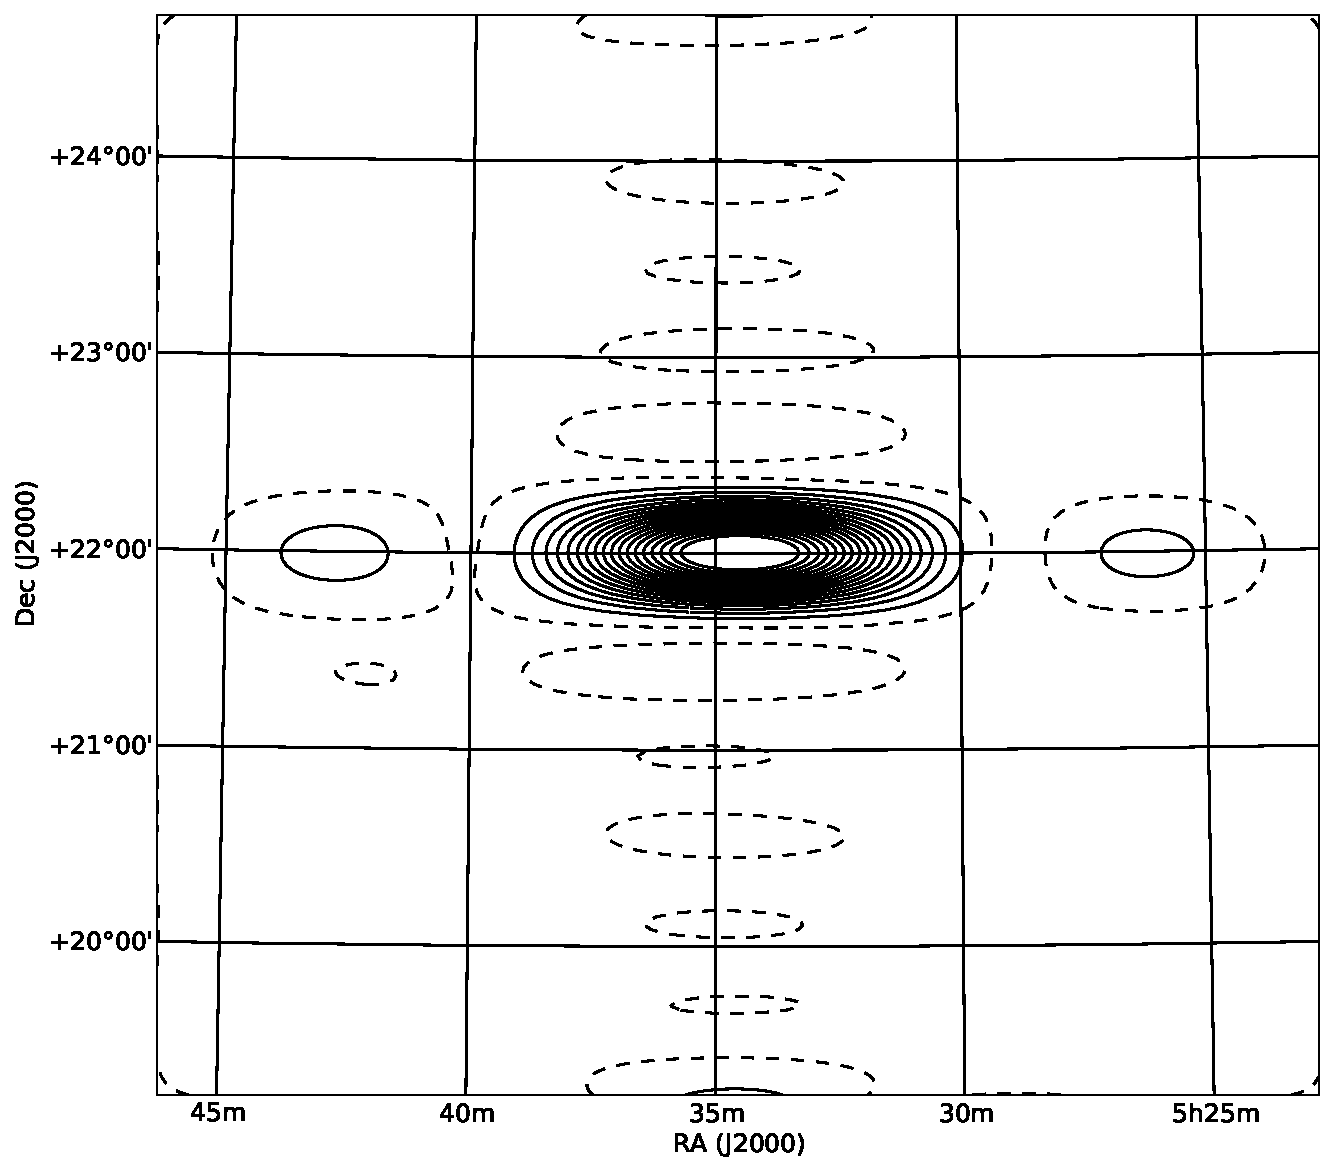
\includegraphics[scale=0.3]{{graphics/fx/corr.2455996.22803.tau.s.ms.natural.CORRECTED_DATA.channel.1ch}.pdf}
    \label{fig:fx_tau_natural}
    }
    \hspace{10pt}
    \subfloat[Dirty image with uniform weighting of the point source Taurus A.]{
    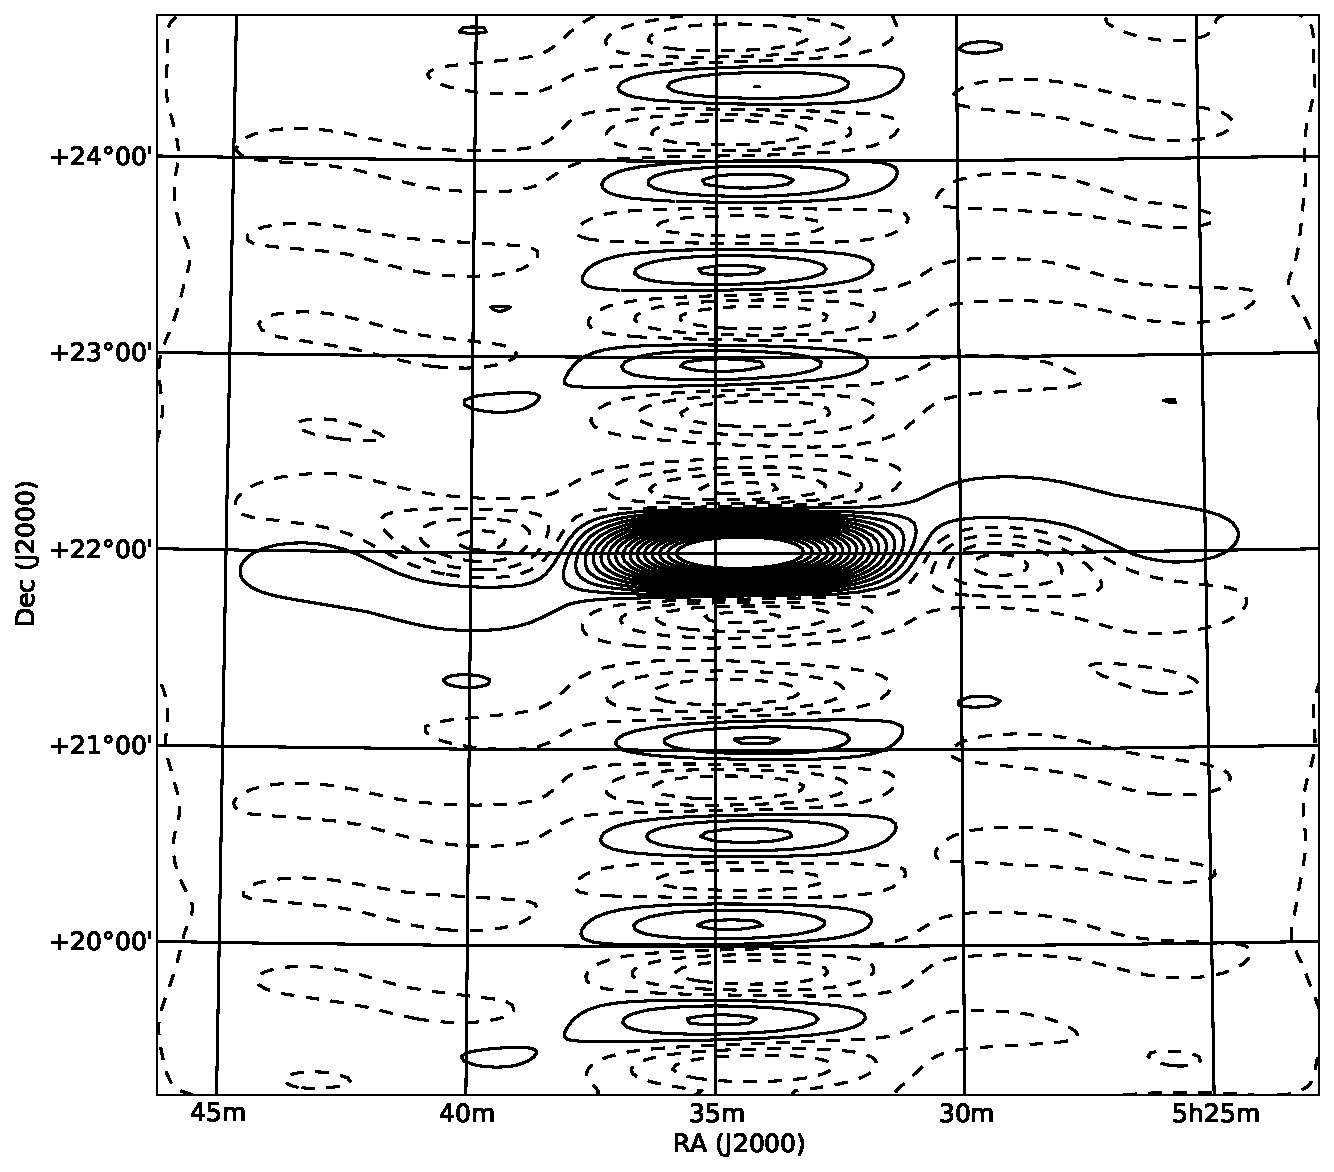
\includegraphics[scale=0.3]{{graphics/fx/corr.2455996.22803.tau.s.ms.uniform.CORRECTED_DATA.channel.1ch}.pdf}
    \label{fig:fx_tau_uniform}
    }
    
    \caption{Natural versus uniform weighting of a point source.
    }
    \label{fig:fx_weighting}
\end{figure}

\section{Spatial FFT Results}
\label{sfft_results}

Observations with the FX correlator of various astronomical sources has verified the array, analogue and digital hardware is functioning as expected.
We will use the FX correlator observations as a baseline to compare the results of observations from the spatial FFT imager.
In the ideal case, observations using the spatial FFT will be identical to observations using an FX correlator.
The spatial FFT imager has the effect of averaging together all identical spacing baselines but the same correlation is performed in both instruments.
Zero padding the data in the spatial FFT preserves the phase information which allows the beams to be transformed into correlations.
Though we have the advantage of applying complex gains after observations with the FX correlator.
The variation in complex gains from when they were derived and when the observations with the spatial FFT imager was performed will introduce the leading error in the data.
We start this section by discussing the calibration methods used and how the derived complex gains vary.

\subsection{Calibration Methods}
\label{calibration}

The operation of the spatial FFT imager turns all redundant baselines into a single unique baseline which makes pre-measurement calibration essential to producing a good observable.
To derive gain coefficients a calibration method is applied to the FX correlator data for an observation of a bright point source.
Deriving the complex gain terms to be applied to the antennas can be achieved with any desired calibration method.
In initial observations the column ratio gain estimation method from \citep{gaindecomp} was used to compute a per channel, per antenna complex gain terms.
The figure \ref{fig:sfft_calibration} shows an observation of Taurus A with and without gains applied during observation.

%SFFT correlations of Tau/3c144 before and after calibration
\begin{figure}
    \centering
    \subfloat[Dirty image of Tau/3c144 formed before applying complex gain calibrations in the F-Engine for the spatial FFT. The uncalibrated phases spread the power through out the image.]{
    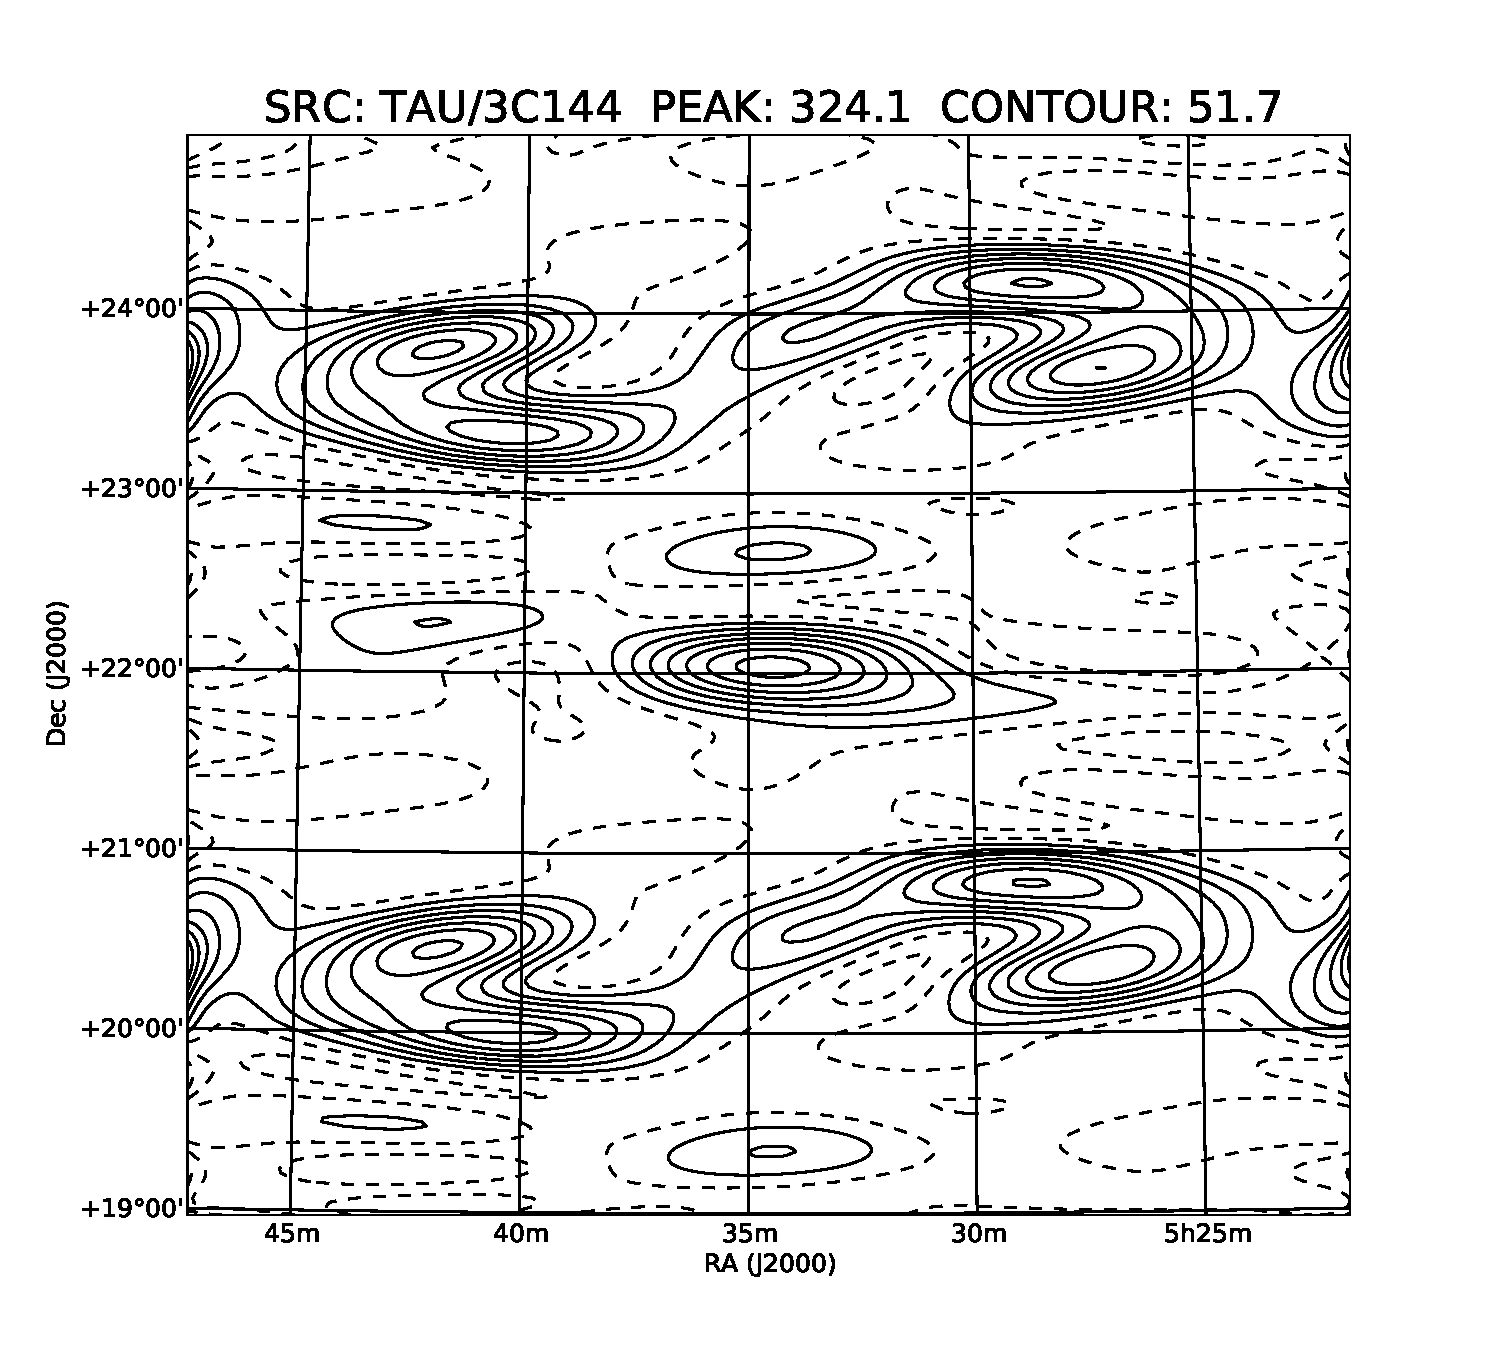
\includegraphics[scale=0.3]{{graphics/img.2455985.25525.tau.uncal.s.ms.DATA.channel.1ch}.pdf}
    \label{fig:uncal_sfft}
    }
    \hspace{10pt}
    \subfloat[Dirty image of Tau/3c144 with complex gain calibrations applied. This image has a signal to noise ratio around 100, a standard CLEAN method can be used to improve the image dynamic range.]{
    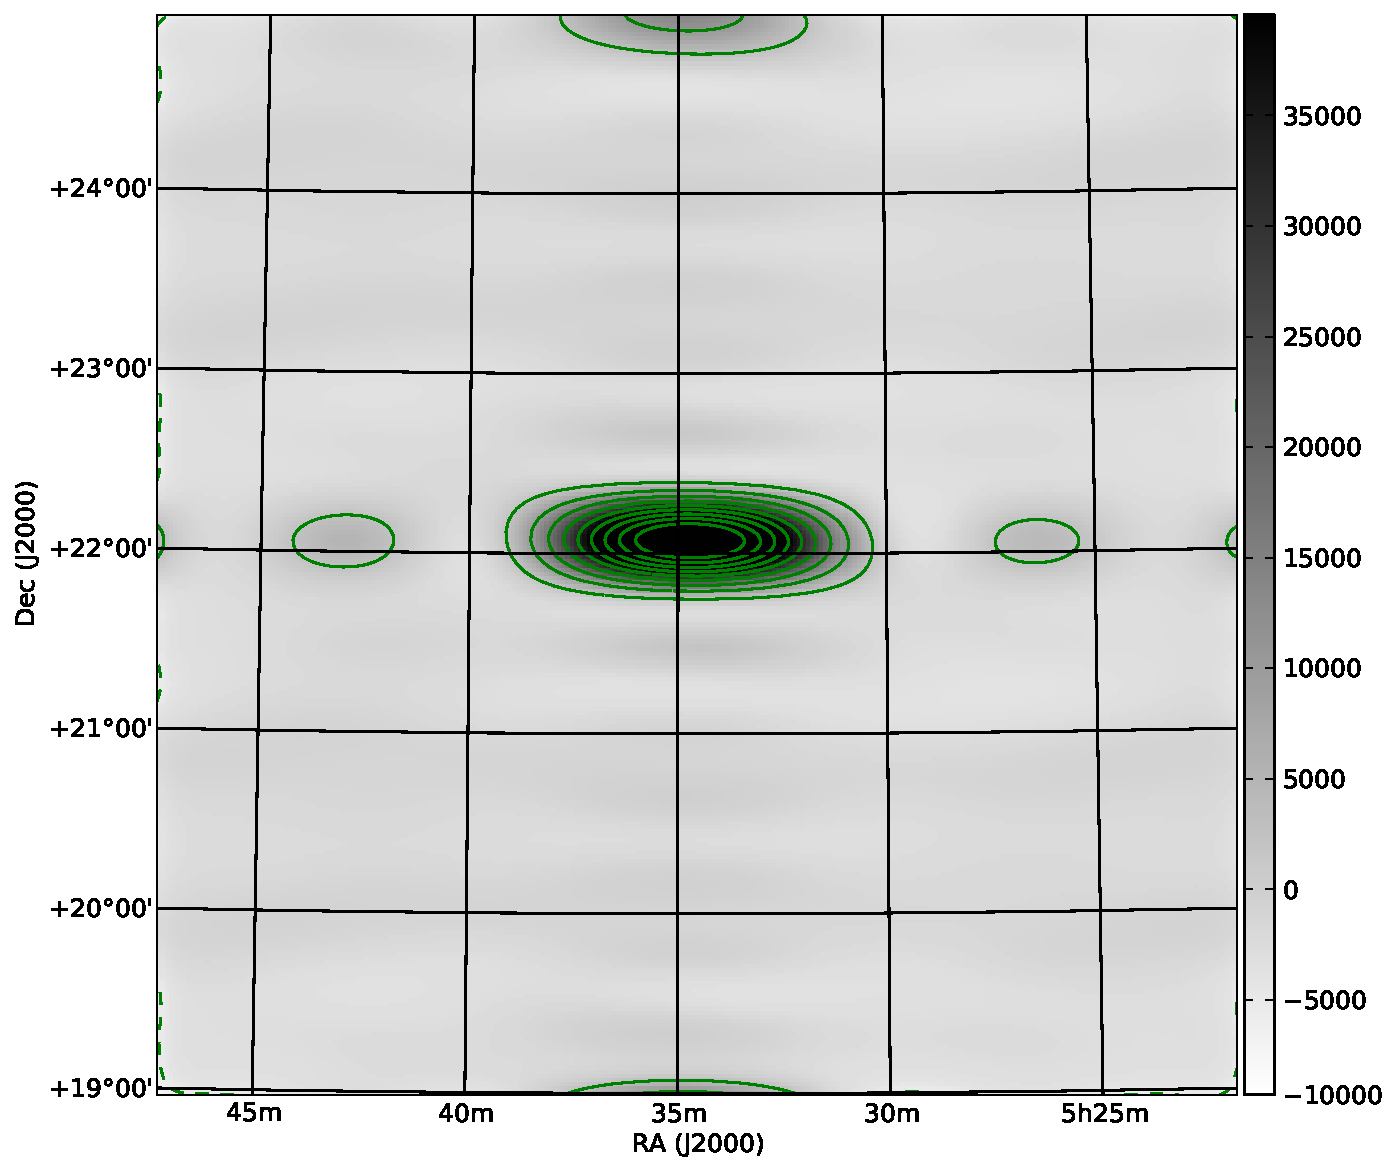
\includegraphics[scale=0.3]{{graphics/img.2455999.21403.tau.cal.s.ms.DATA.channel.1ch}.pdf}
    \label{fig:cal_sfft}
    }
    \caption{After applying complex gain calibration a bright point source such as Tau/3c144 appears similar to the array PSF, and has a significant improvement in the image fidelity compared to the uncalibrated image.
    \label{fig:sfft_calibration}
    }
\end{figure}

The bright sources Cygnus A and Taurus A were used as calibration sources.
With transiting array and a limited field of view these observations can only be made at a set time of day.
Thus gains for a spatial FFT can often only be derived many hours before an observation.
If an array is sufficiently stable over that time period then this does not pose a serious problem.
%what is 'sufficiently stable'?
%variability: source, temp, time of day
%fig: gain variation

%post integration methods: baseline cal for overall amp and phase correction, but can not be used for individual antennas

\subsection{Spatial FFT as a Beamformer}
\label{sfft_beamformer}

%use as a beamformer
%fig:sfft beams on the sky
%fig:beam crossing
%pulsar machine

\subsection{Spatial FFT as a Correlator}
\label{sfft_correlator}

The output of the spatial FFT is a set of 128 complex beams which can be converted to uv sampled baselines by performing an inverse FFT.
In total 52 unique baselines are produced along with the auto correlation.
Each spatial FFT baseline is a linear combination of antenna pair baselines at the same antenna spacing, for a given frequency channel.
For the case of the spatial FFT we will call them effective baselines.
Once in the effective baseline correlation format the same pipeline that is used for the FX correlator is used to convert the data into measurement sets.

Due to the calibration limitation of the data no post observation calibration is applied.
The flux scale is set by using the flux scale from the FX images.
This scale can be set during the observation or in post processing since it is a baseline independent amplitude scaling.
Figures \ref{fig:sfft_tau_dirty} and \ref{fig:sfft_tau_clean} show the dirty and clean images of Taurus A during a properly calibrated observation.
The signal to noise of the images are comparable to that of the images formed with the FX correlator during the same observation, fig. \ref{fig:fx_tau}.
We expect both instruments to produce comparable results, though there has been an open question as to how 'good' the real time calibration must be and how often this calibration must change.
In the following section we look at the results of observations from both instrument to understand to the quality of images produced by the spatial FFT relative to that of the FX correlator.

\subsubsection{Image Comparison}
\label{fx_sfft_image_comp}

\begin{figure}
    \centering

    \subfloat[Dirty image of Taurus formed from the spatial FFT imager, the flux scale has been fixed to the scale based on the same image from the FX correlator. The dynamic range,$\sim100$, is less than that of the FX correlator image, $\sim150$.]{
    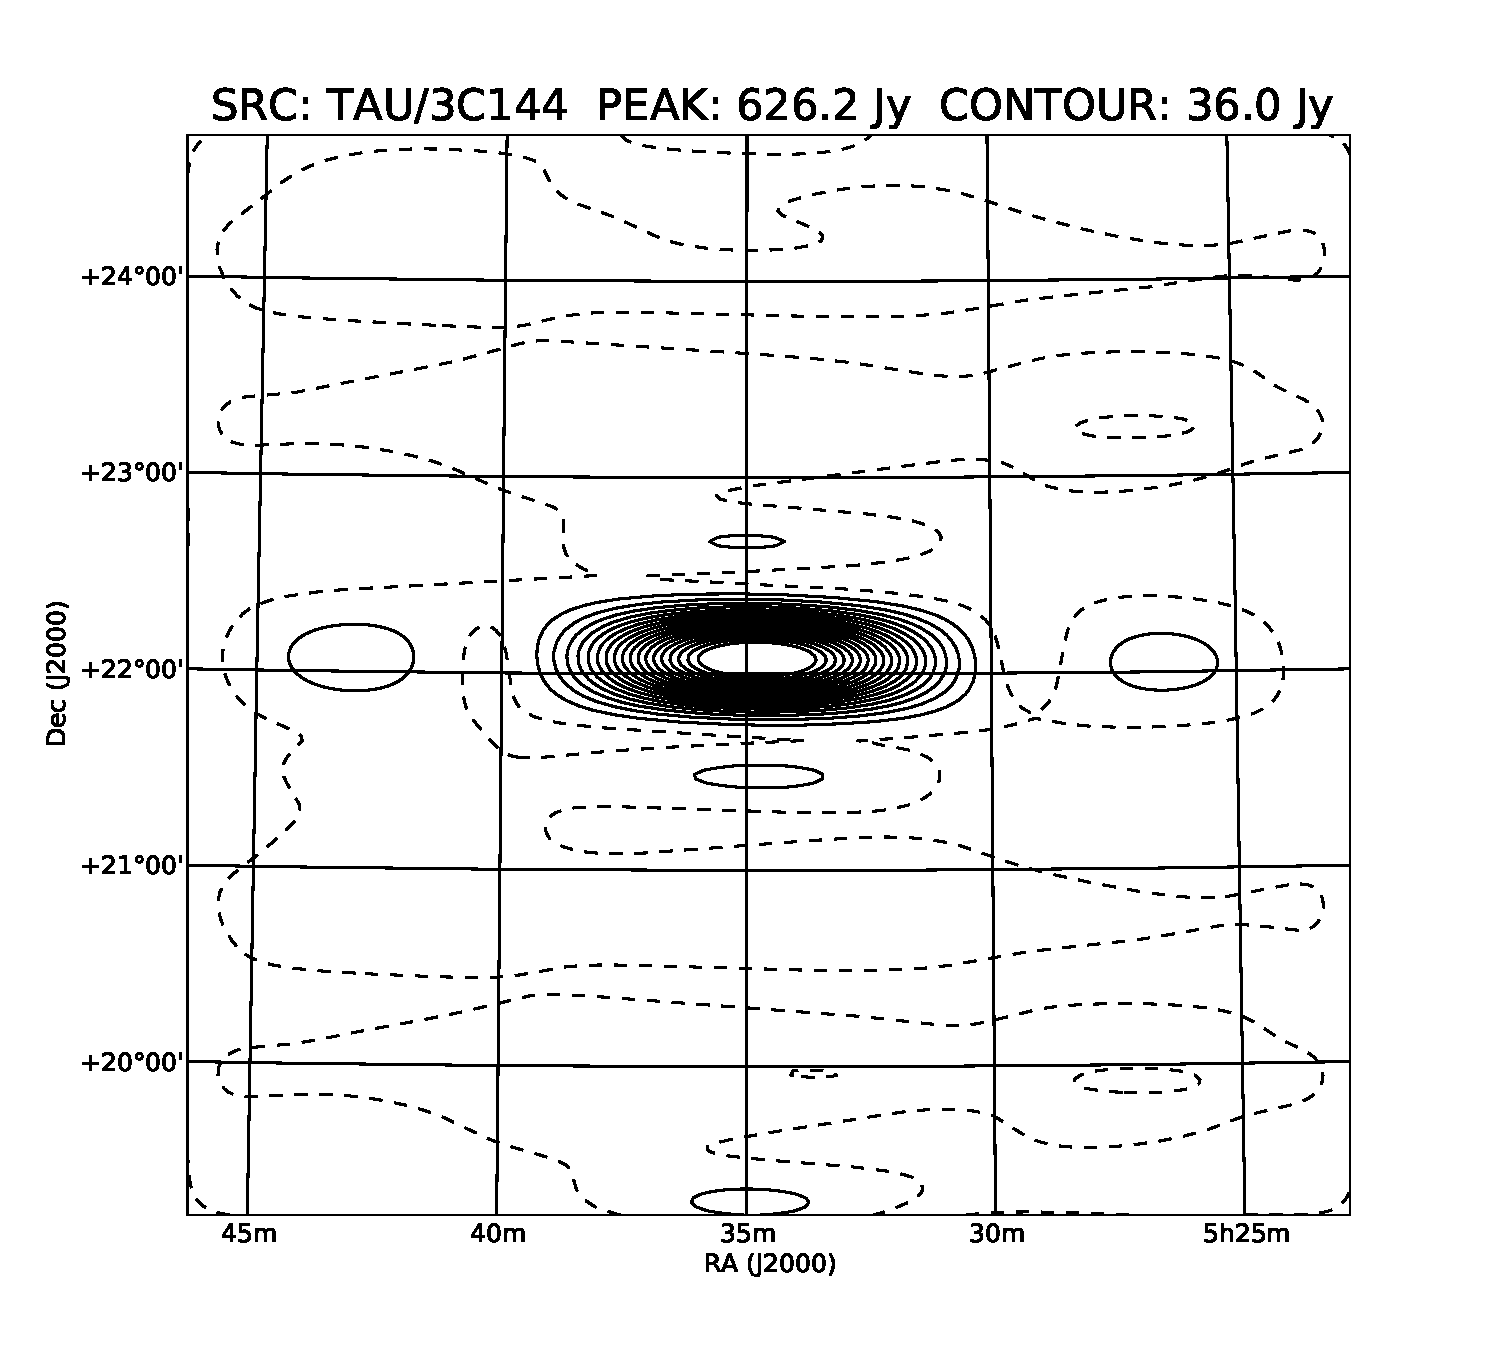
\includegraphics[scale=0.3]{{graphics/sfft/img.2455996.22807.tau.s.ms.DATA.channel.1ch}.pdf}
    \label{fig:sfft_tau_dirty}
    }
    \hspace{10pt}
    \subfloat[Cleaned image of the Taurus field. The cleaning process brings the dynamic range up to around 300, similar to the value from the FX correlator image in fig. \ref{fig:fx_tau_clean}.
    A notable feature about the the cleaned images from the spatial FFT is the apparent low level skewing of the image, particularly in the east-west direction.]{
    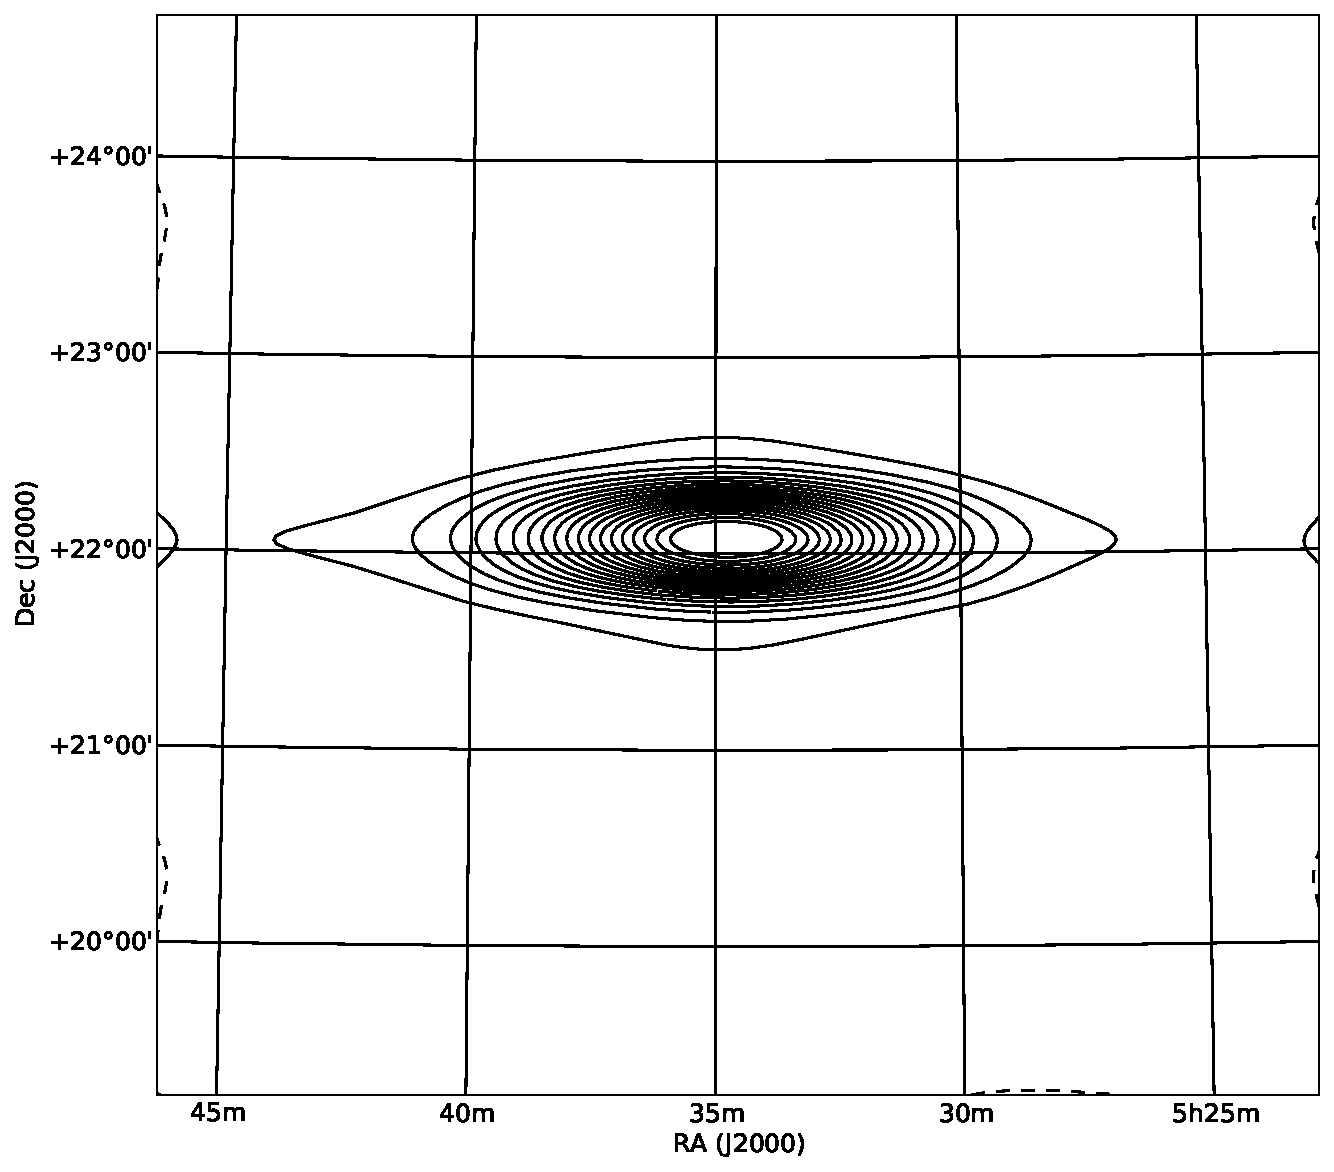
\includegraphics[scale=0.3]{{graphics/sfft/img.2455996.22807.tau.s.ms.DATA.channel.1ch.restored}.pdf}
    \label{fig:sfft_tau_clean}
    }
    
    \label{fig:sfft_tau}
    \caption{The images produced by the spatial FFT imager are comparable in noise and dynamic range to those produced with calibrated FX correlator data.
    }
\end{figure}

A number of 3C source fields have been imaged with concurrent observations with the FX correlator and spatial FFT imager, figures \ref{fig:fx_sfft_set1} and \ref{fig:fx_sfft_set2}.
To make a comparison between images we define the dynamic range of each image to the peak flux divided by the standard deviation of the noise in a empty region of the image.
Selecting an empty region of an image can greatly influence the dynamic range if there is low level structure, we took care to select a few regions per image to find a representative region.
The same region was then used for images from both the FX correlator and the spatial FFT imager as to avoid bias.
Though this is a simple way to define and determine the noise level and dynamic range we are not interested in the absolute flux of the images.
We are interested in the difference in image quality between the two sets of results.
In table \ref{tbl:src_flux} we list a number of 3C sources along with their measured flux and noise levels.
For these snapshot images the spatial FFT produces essentially the same results as the FX correlator.

\begin{table}
\begin{center}
\begin{tabular}{|c||c|c|c|c|}
\multicolumn{5}{|c|}{Measured Source Flux and Noise Levels}\\
\hline
Source & 3C Flux (Jy) & Peak Flux (Jy) & FX Noise Level (Jy) & SFFT Noise Level (Jy) \\ \hline
    3C10  &   134 &  67.2 & 1.1 & 1.3 \\
    3C48  &    47 &  27.3 & 0.9 & 0.8 \\
    3C123 &   175 &  91.1 & 2.1 & 1.9 \\
    3C144 &  1420 & 729.5 & 2.0 & 2.5 \\
    3C157 &   210 & 116.5 & 1.6 & 2.3 \\
    3C196 &    59 &  34.6 & 0.9 & 1.7 \\ \hline
\end{tabular}
\caption{Noise level for various 3C sources calculated for images formed with data from the FX correlator and the spatial FFT imager.}
\label{tbl:src_flux}
\end{center}
\end{table}

Even though the results have comparable dynamic range in the spatial FFT images there is a noticeable distortion.
The cleaned image of Taurus, fig. \ref{fig:sfft_tau_clean}, begins to form points at the low levels, primarily in the east-west direction.
This effect can also be seen in a number of the 3C images in figures \ref{fig:fx_sfft_set1} and \ref{fig:fx_sfft_set2}.
This effect is not noticeable until the image has been cleaned.
The dynamic range of the images does not fully describe the difference between a pair of images.
We must look at the individual baselines to see how the two instruments compare.

\subsubsection{Baseline Phase Comparison}
\label{fx_sfft_bl_comp}

The distortions in the spatial FFT images should appear as a higher phase noise in the effective baselines compared to the FX correlator baselines.
There are two baselines in the array, (0,31) and (3,28), which are unique.
The spatial FFT and the FX correlator should produce the same result for these baselines.
Figure \ref{fig:bl_phase_1} shows the phase for this baseline as calculated from both instruments.
Both are similar but the spatial FFT has a higher noise standard deviation.

\begin{figure}
    \centering
    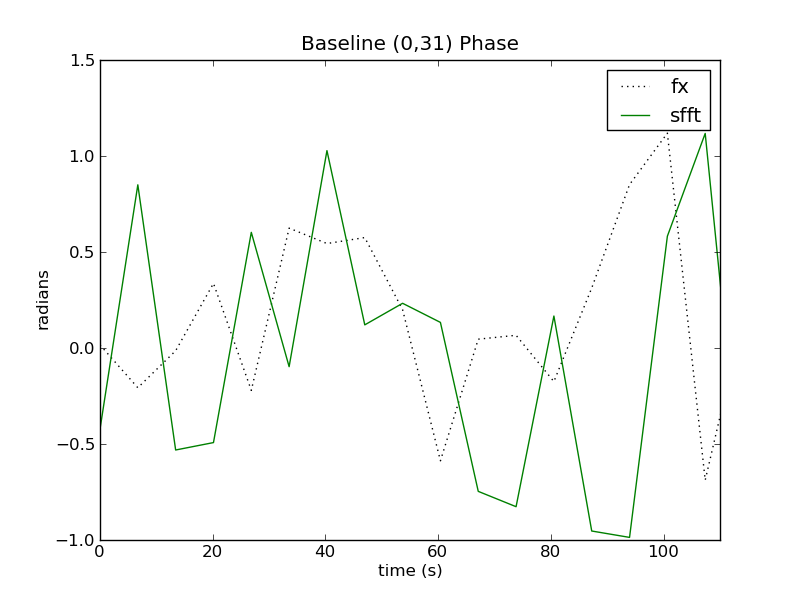
\includegraphics[scale=0.6]{{graphics/bls/phase_plot_0_31_3c48}.png}
    \caption{The (0,31) baseline is the one of the non-redundant baselines in the array.
    Both instruments should produce a baseline with similar noise characteristics.
    But the standard deviation of the noise from the spatial FFT observation is $48\%$ higher than the FX correlator.
    }
    \label{fig:bl_phase_1}
\end{figure}

If we look at a highly redundant baseline, such as (0,4), we expect the individual FX baselines to have a higher noise figure than the spatial FFT effective baseline, figure \ref{fig:bl_phase_0}.
The effective FX baseline which is an average of same redundantly spaced baselines should be the same as the effective spatial FFT baseline.
This is shown to be correct, but again the spatial FFT effective baseline has a higher noise characteristic.

\begin{figure}
    \centering
    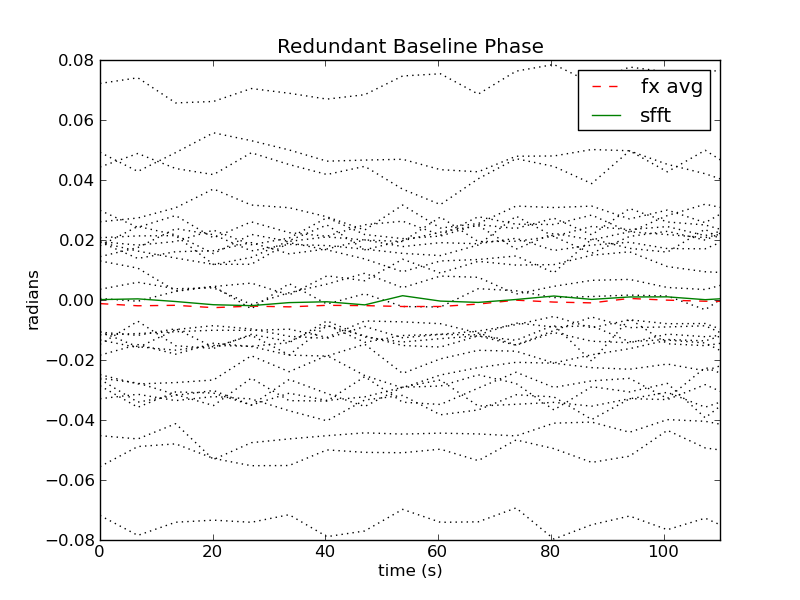
\includegraphics[scale=0.6]{{graphics/bls/phase_plot_0_4_tau}.png}
    \caption{Phase comparison of the FX correlator baselines which are redundant with the (0,4) antenna spacing and the corresponding spatial FFT baseline.
    The lines are: redundant FX correlator baselines(dotted), spatial FFT combined baseline (solid), all the FX baselines averaged together(dashed).
    For this baseline, the spatial FFT baseline fits the averaged FX baseline well but has $\sim35\%$ more noise.
    }
    \label{fig:bl_phase_0}
\end{figure}

If we look at the noise standard deviation for all the baselines during an observation we see the individual FX baselines have a constant  characteristic, figure \ref{fig:bl_phase_noise}.
If the FX baselines are averaged together based on their redundancy the noise decreases with redundancy as expected.
The spatial FFT effective baseline noise also falls off with an increase in redundancy.
Yet, the noise standard deviation is higher on every baseline compared to the averaged FX baselines.

\begin{figure}
    \centering
    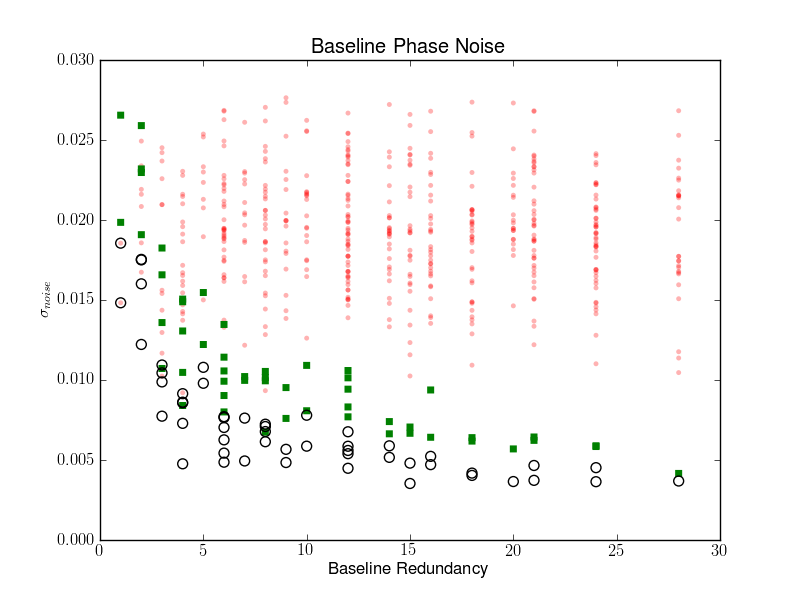
\includegraphics[scale=0.6]{{graphics/bls/tau_bls}.png}
    \caption{Phase noise for each baseline during an observation plotted against the the number of redundant baselines.
    Small dots are the 496 FX correlator baselines.
    Circles are the FX correlator baselines after averaging together sets of equal spacing baselines.
    This expectedly decreases as $\frac{1}{\sqrt{n}}$ on the more redundant spacings.
    Squares are the spatial FFT baselines, which are effectively an average of all the redundant spacing baselines.
    The spatial FFT baseline noise also decreased at a rate similar to the averaged FX correlator baselines.
    Though the spatial FFT phase noise is $.48\pm.26$ higher than the FX averaged baselines in this data set.
    }
    \label{fig:bl_phase_noise}
\end{figure}

\subsubsection{Error Effects}
\label{sfft_error}

In the extreme case where a set of antennas are not functioning the effects on the spatial FFT imager are significant.
With an FX correlator a `bad' baseline or antenna can be flagged in the data during post processing.
If we assume all the antennas in an array are identical and each baseline has an nominal phase noise of $\sigma_{nom}$ then a `bad' baseline can be defined as having a noise level of $N$ times higher than the nominal noise level, $N\sigma_{nom}$.
For a spacing with $m$ redundant baselines the combined noise is $\sigma_{bl}=\sigma_{nom}\sqrt{m}$.
If there are $B$ bad baselines which are flagged the noise becomes $\sigma_{bl}=\sigma_{nom}\sqrt{(m-B)}$.
In the case of the spatial FFT all the baselines are summed together before a baseline can be flagged.
Then the baseline noise is $\sigma_{bl}=\sigma_{nom}\sqrt{m-B}+\sigma_{nom}N\sqrt{B}$.
A malfunctioning antenna corrupts any effective baselines it is part of, and can not be flagged and filtered in post processing.
The stability of every antenna must be checked during an observation or the observation could be a waste.
It should be noted that in the case of a known bad antenna, that antenna can be flagged during an observation and dropped.

This is the effect we see in the effective spatial FFT baselines.
Though the baselines are not `bad', each baseline has a different noise characteristic.
By combining them we can not use self calibration to apply per antenna calibration later to reduce the noise like is done with the FX correlator.
The initial phase calibration from a bright source is the same for the both instruments, though the gains are applied during the observation in the spatial FFT case and in post processing for the FX correlator.
The additional calibration on the FX data by solving for a sky model solution further improves the image quality.

\section{Discussion}
\label{discussion}

We have shown that the spatial FFT imager produces correlations similar to that of a traditional FX correlator.
Though with an increase in noise which we attribute to the accuracy of the gain calibration.
The BEST-2 array is limited in the ability to improve the calibration.
Bright sources are needed in the field of view to derive calibrations.
A more advanced calibration method which can take into account multiple sources would allow more fields to be used for calibration and improve the time difference between calibration observation and science observation.

For low frequency dipole arrays which have a very large field of view then there will always be bright sources in the field to calibrate off.
With a fast enough calibration algorithm a small correlator can be used to derive gains on short timescales(minutes, seconds) and apply them to the spatial FFT.

With the successful installation and testing with the spatial FFT imager on the BEST-2 array we working on developing the system further for science observations.
Medicina is involved with space debris tracking using BEST-2 in a beamformer mode.
The spatial FFT provides all beams within the field of view.
This would improve the ability to detect and track space debris with the array.
As noted earlier the beams have been used with a dedispersion machine to detect various pulsars.
Work on this is in further development.

%images: compare images of FX and SFFT
\begin{figure}
    \centering

    \subfloat[]{
    %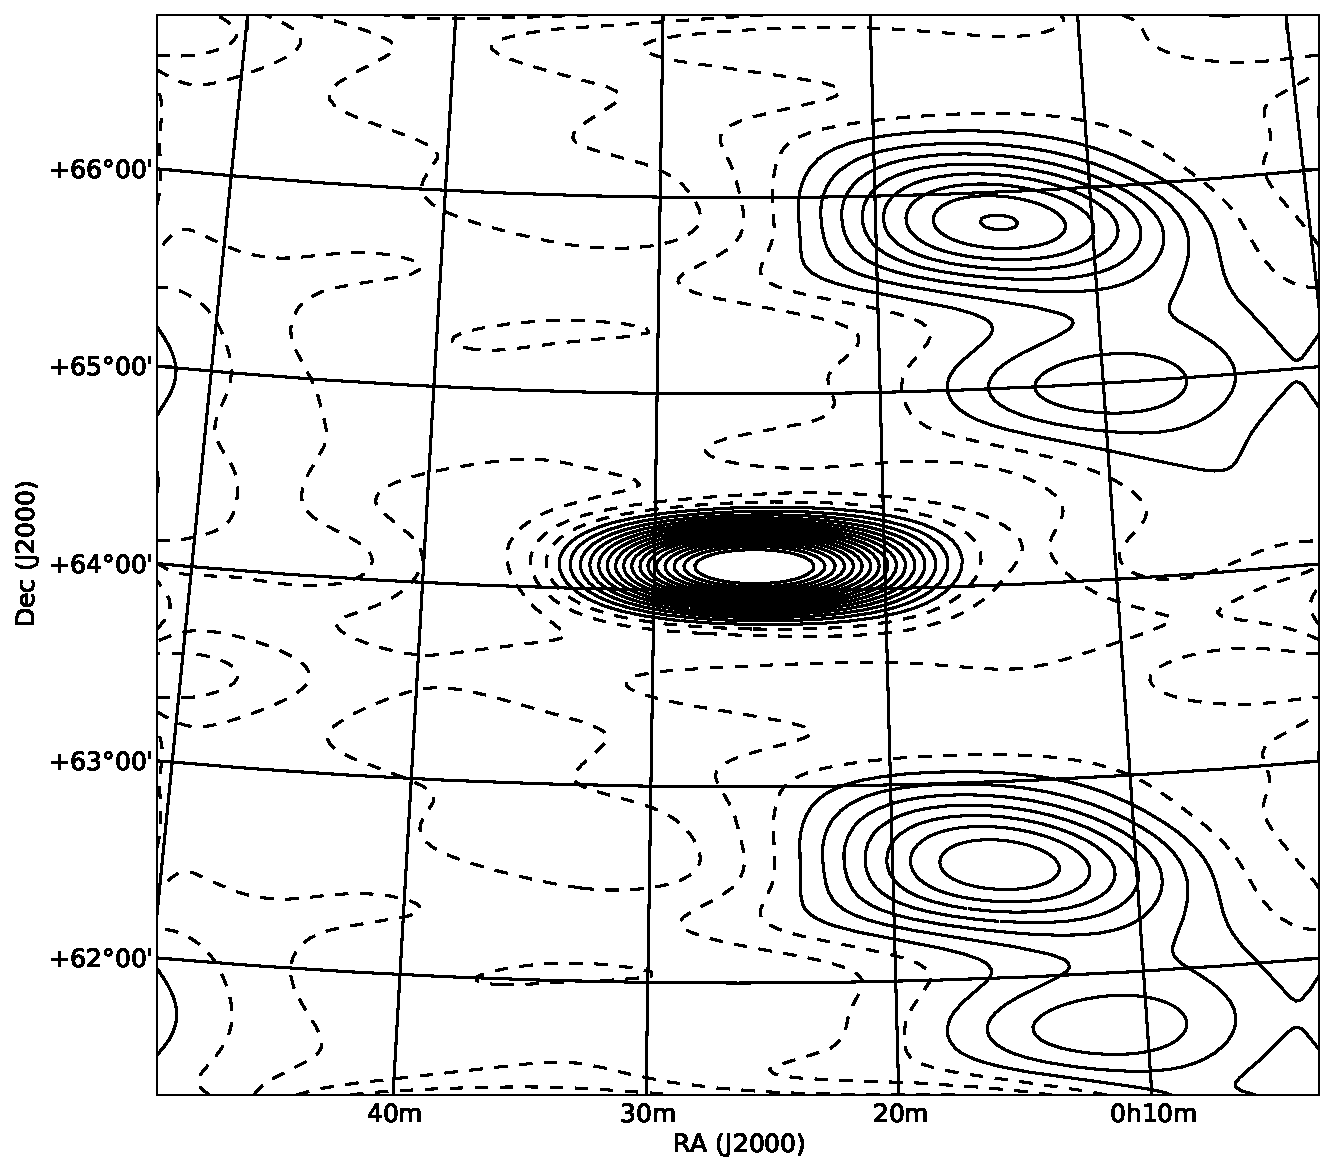
\includegraphics[scale=0.3]{{graphics/3c10/corr.2455996.01891.10.s.ms.CORRECTED_DATA.channel.1ch}.pdf}
    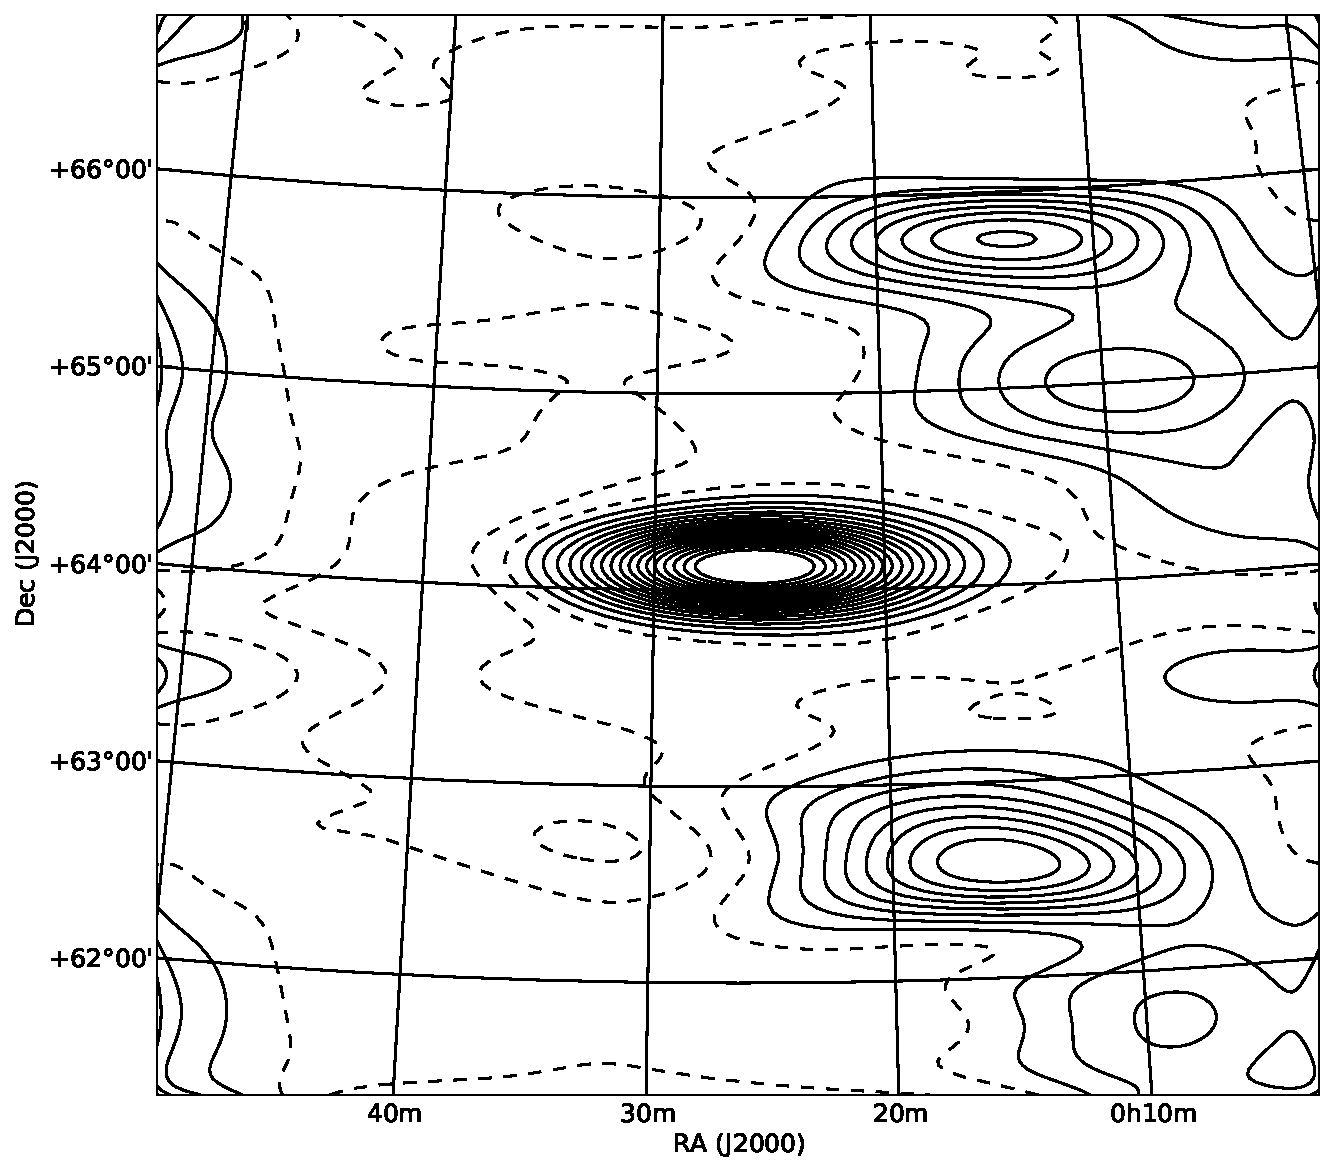
\includegraphics[scale=0.3]{{graphics/3c10/corr.2455996.01891.10.s.ms.CORRECTED_DATA.channel.1ch.restored}.pdf}
    \label{fig:fx_3c10_dirty}
    }
    \hspace{10pt}
    \subfloat[]{
    %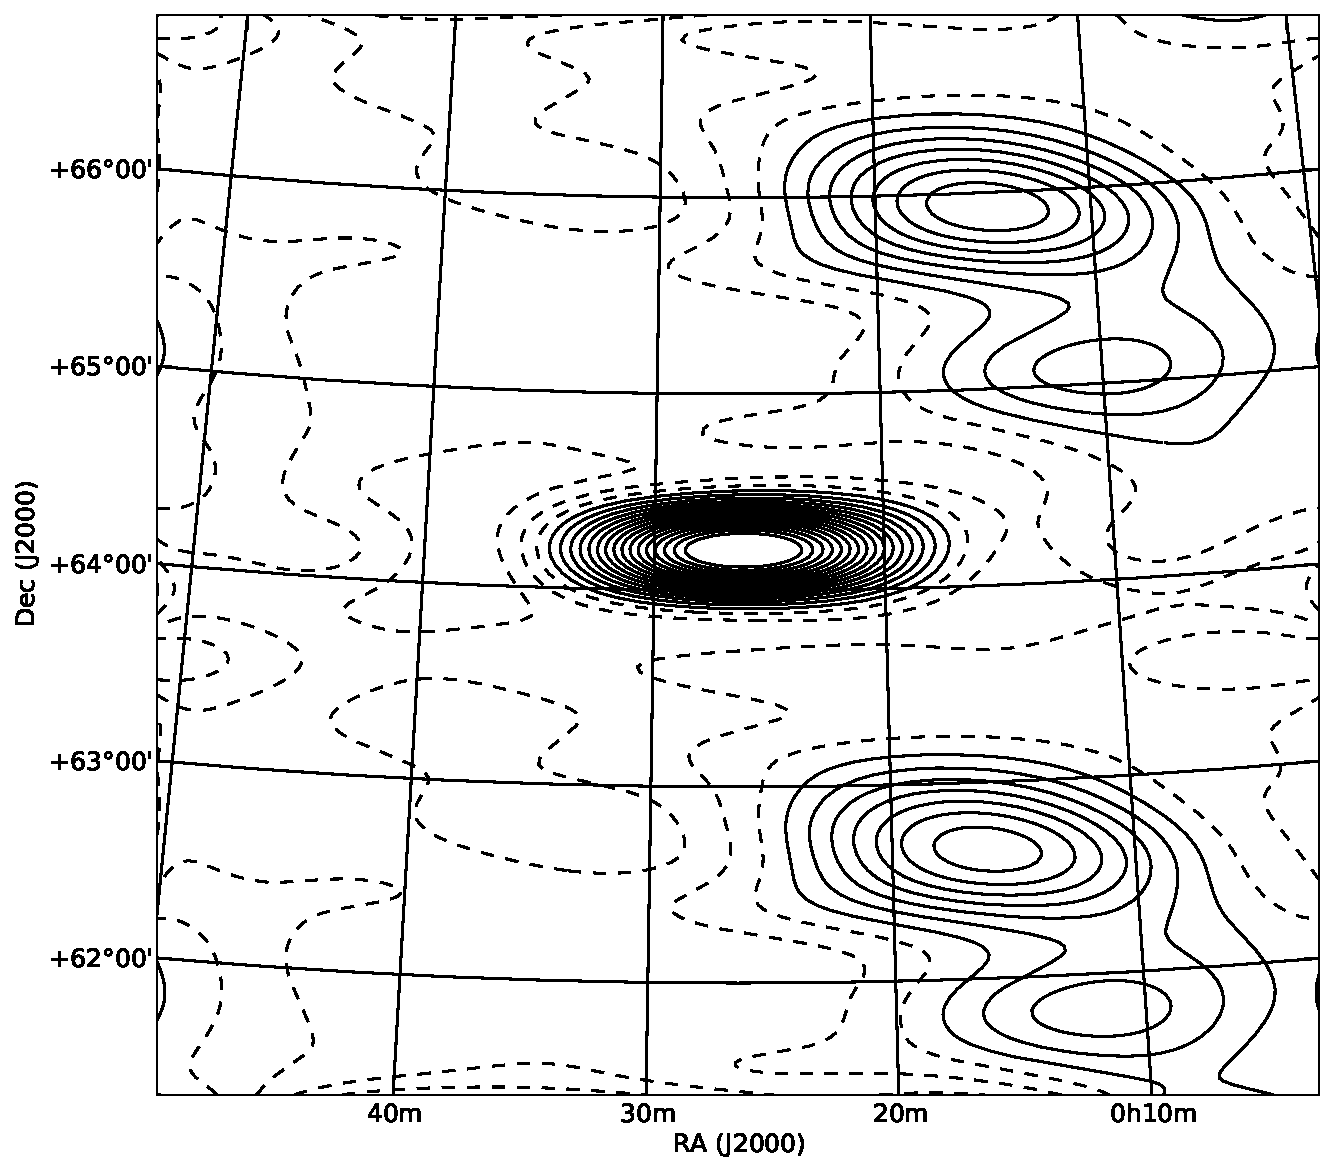
\includegraphics[scale=0.3]{{graphics/3c10/img.2455996.00424.10.s.ms.CORRECTED_DATA.channel.1ch}.pdf}
    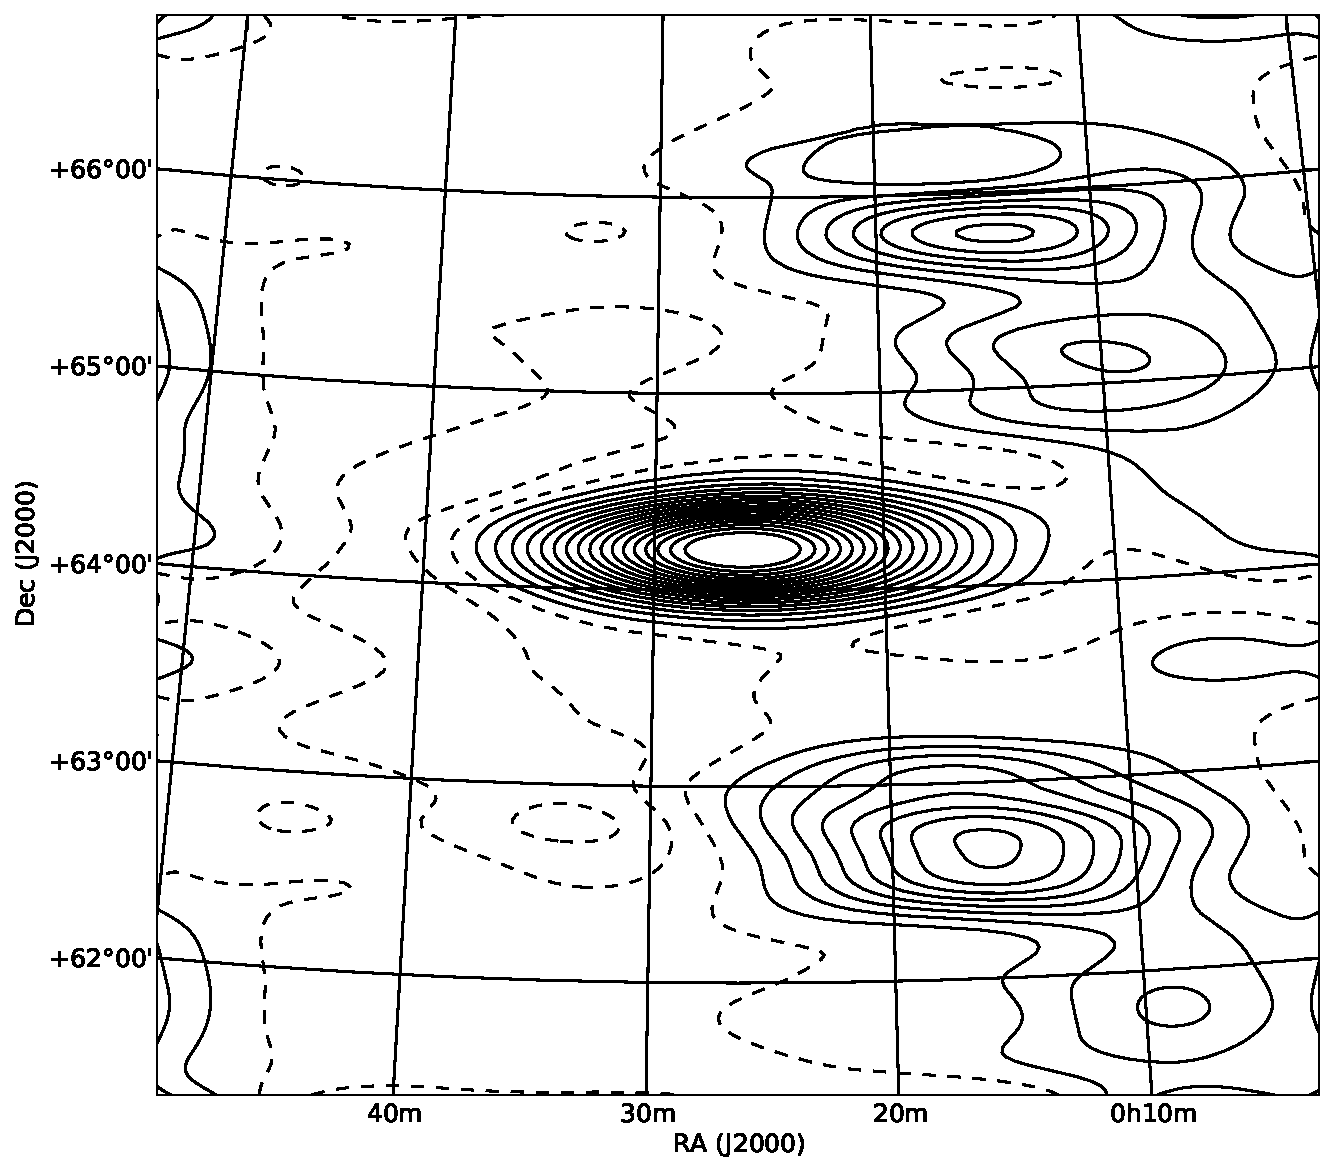
\includegraphics[scale=0.3]{{graphics/3c10/img.2455996.00424.10.s.ms.CORRECTED_DATA.channel.1ch.restored}.pdf}
    \label{fig:sfft_3c10_dirty}
    }
    \vspace{-10pt}

    \subfloat[]{
    %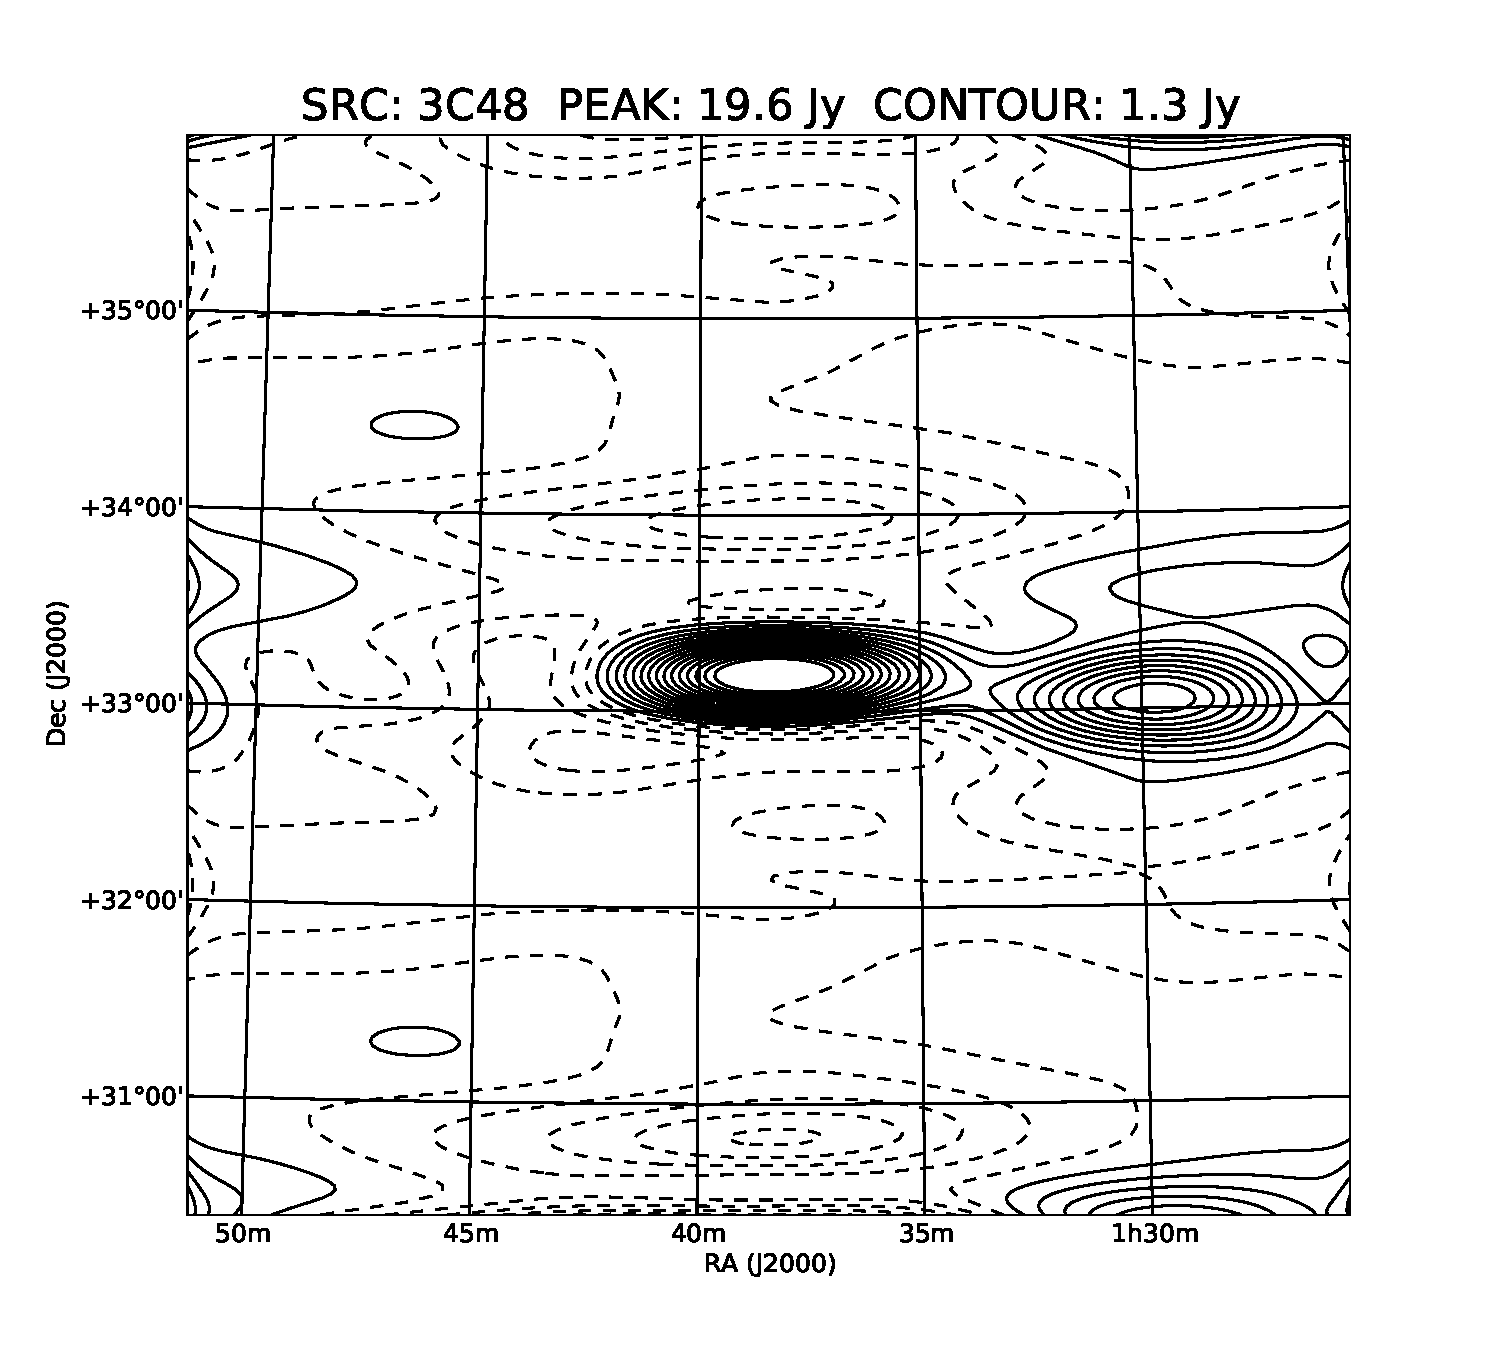
\includegraphics[scale=0.3]{{graphics/3c48/corr.2455996.06793.3c48.s.cal.ms.CORRECTED_DATA.channel.1ch}.pdf}
    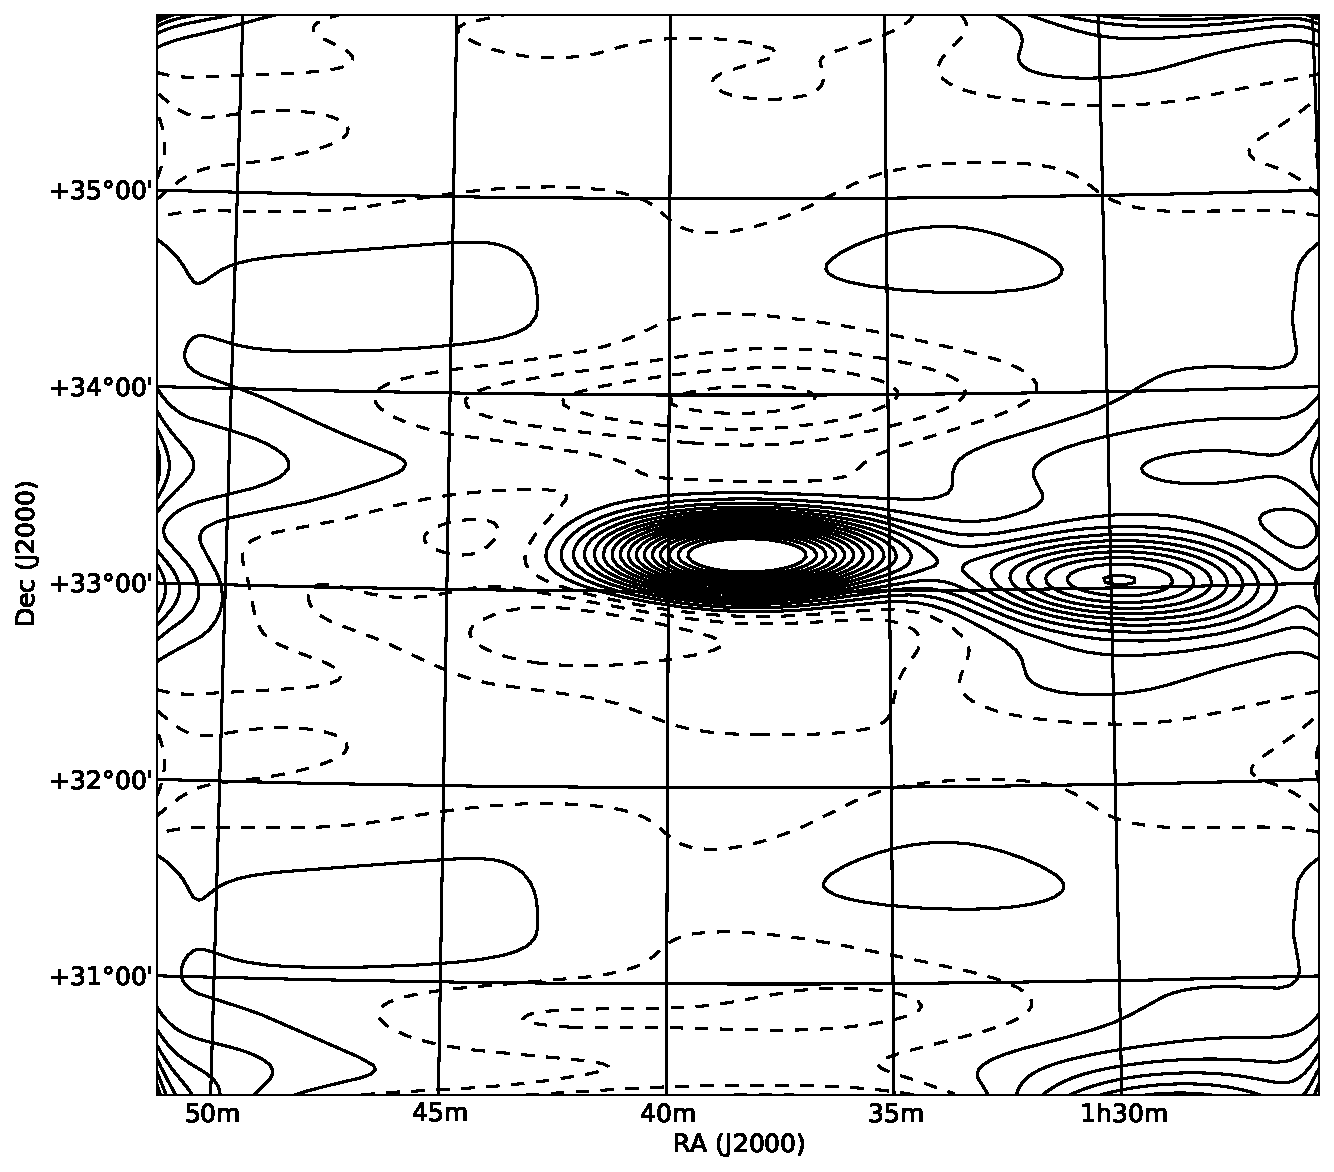
\includegraphics[scale=0.3]{{graphics/3c48/corr.2455996.06793.3c48.s.cal.ms.CORRECTED_DATA.channel.1ch.restored}.pdf}
    \label{fig:fx_3c48_dirty}
    }
    \hspace{10pt}
    \subfloat[]{
    %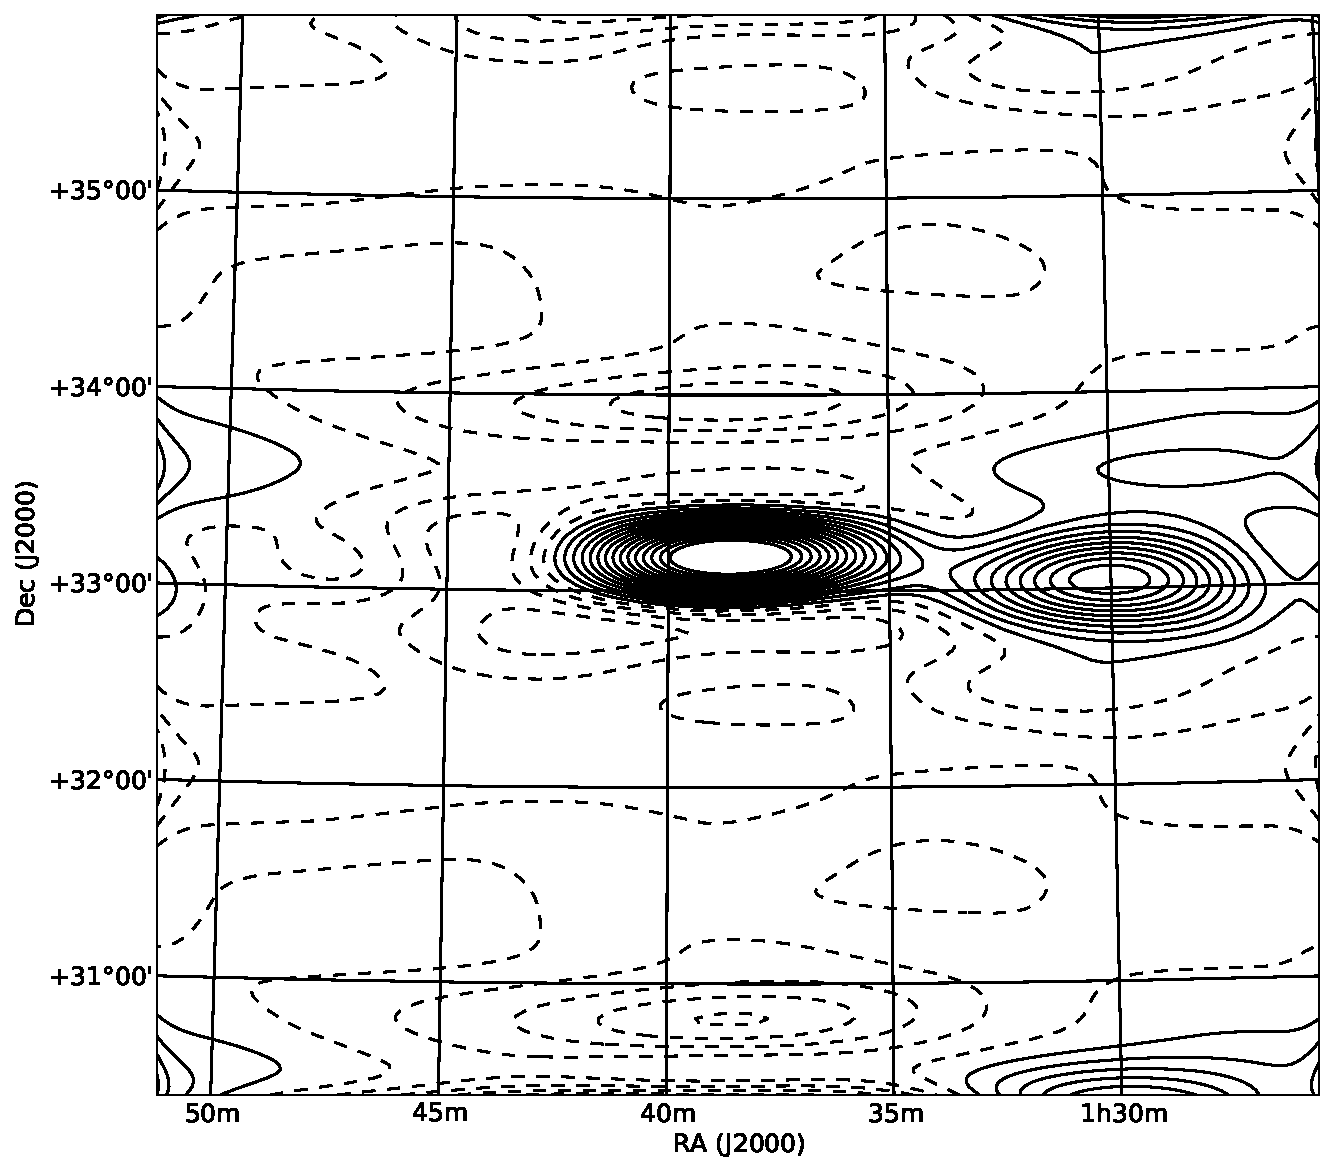
\includegraphics[scale=0.3]{{graphics/3c48/img.2455996.05169.48.s.ms.DATA.channel.1ch}.pdf}
    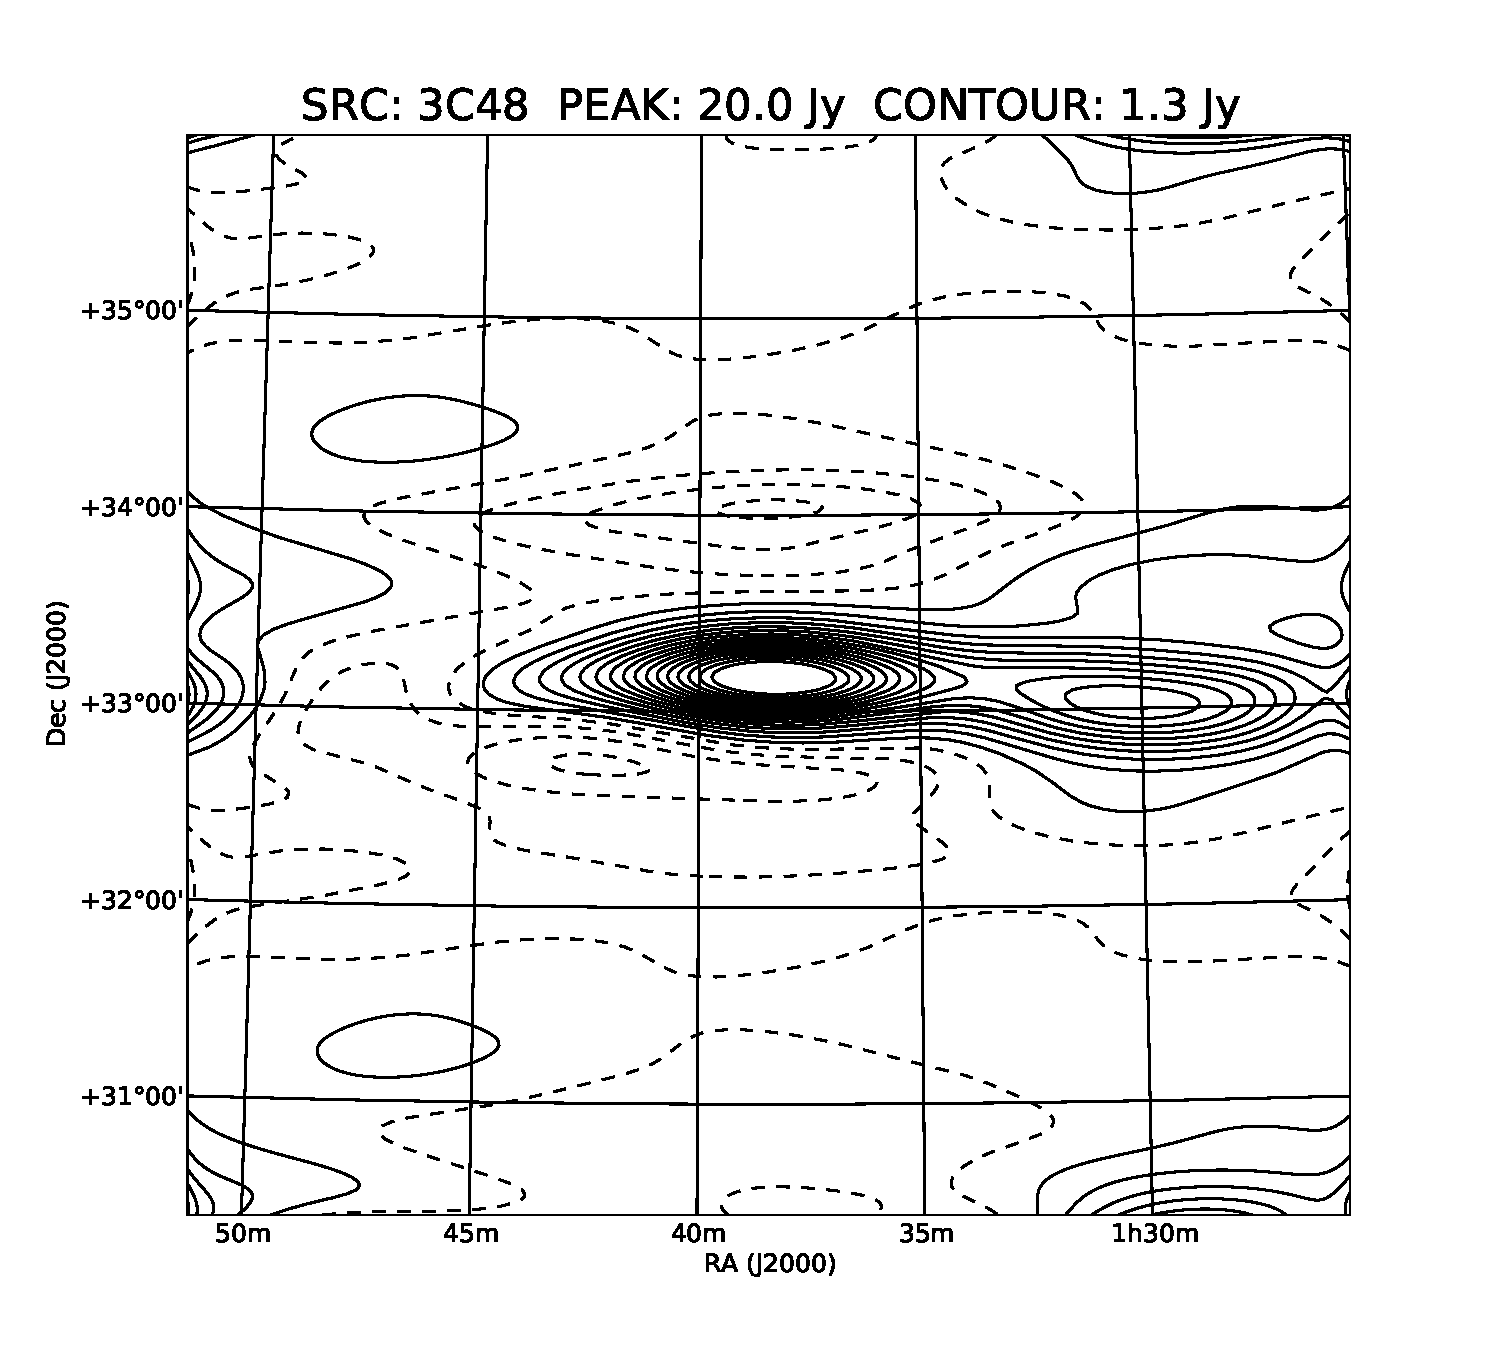
\includegraphics[scale=0.3]{{graphics/3c48/img.2455996.05169.48.s.ms.CORRECTED_DATA.channel.1ch.restored}.pdf}
    \label{fig:sfft_3c48_dirty}
    }
    \vspace{-10pt}
    
    \subfloat[]{
    %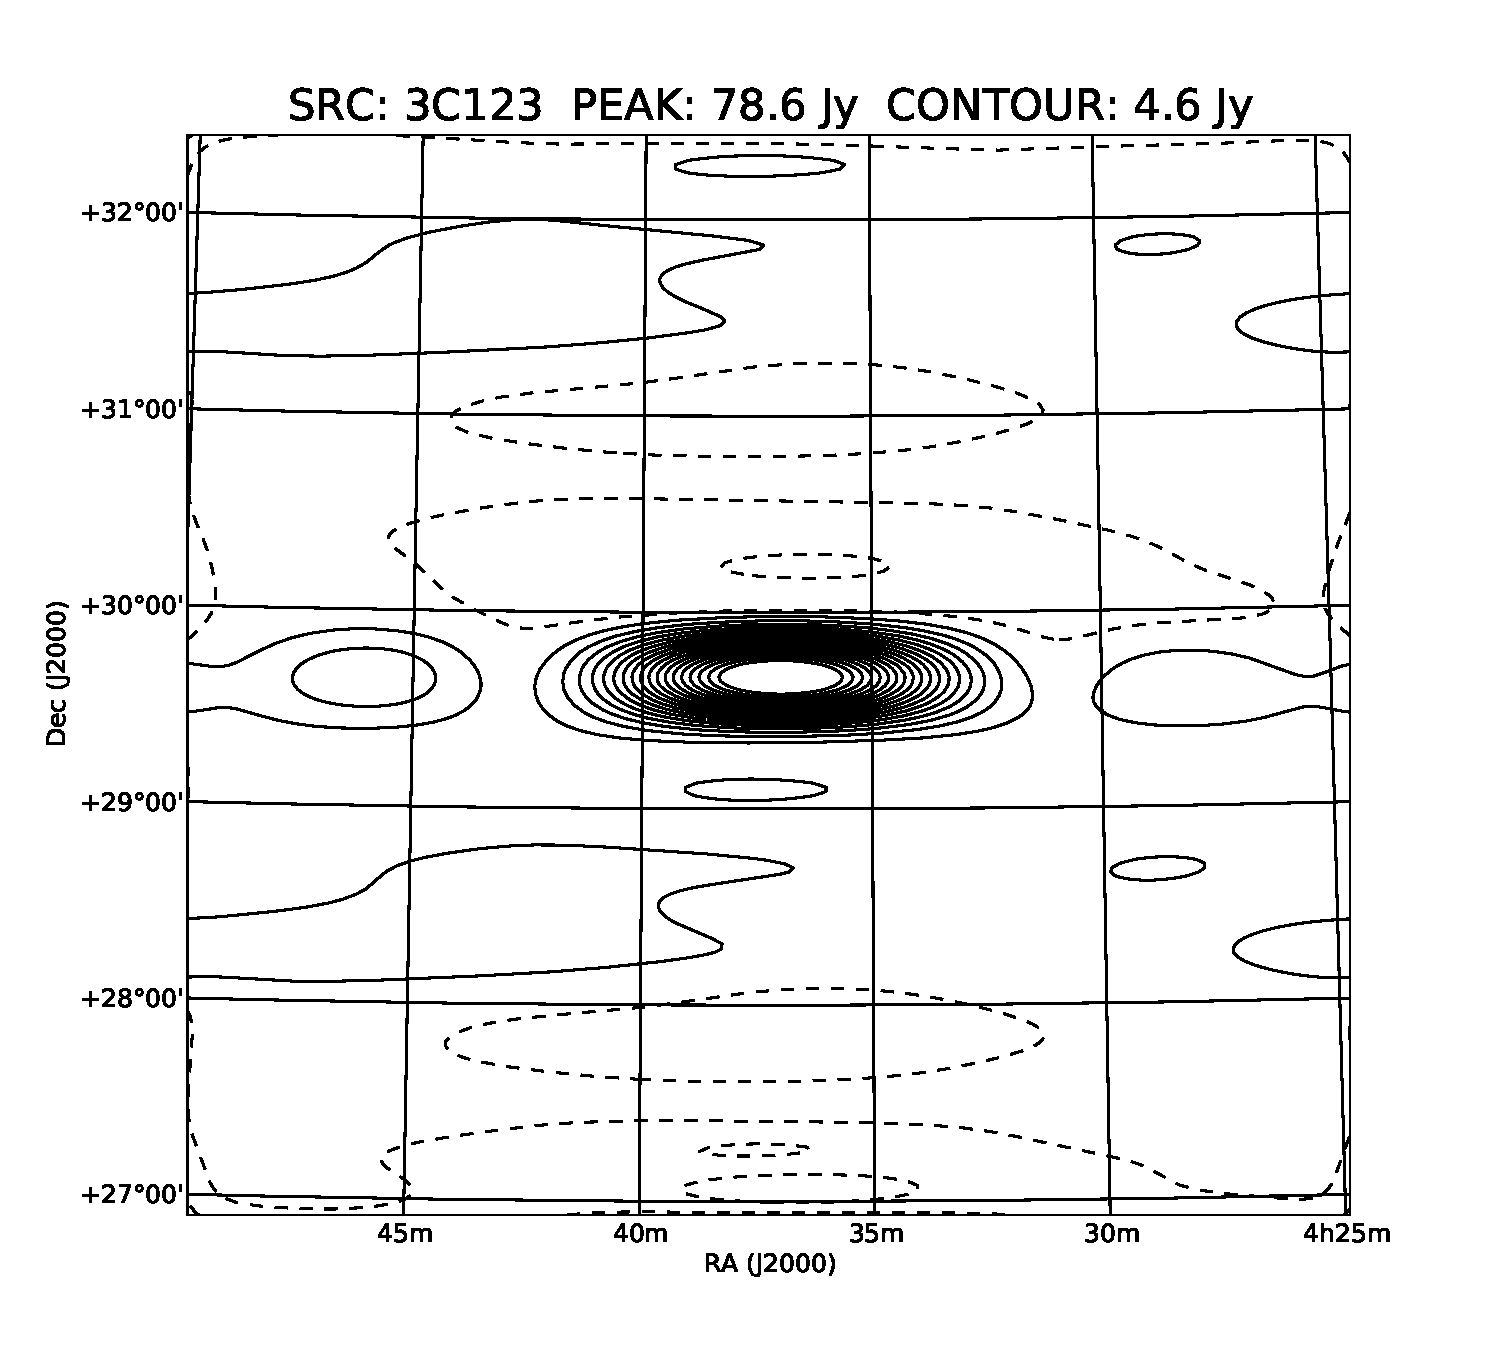
\includegraphics[scale=0.3]{{graphics/3c123/corr.2455996.19182.123.s.ms.CORRECTED_DATA.channel.1ch}.pdf}
    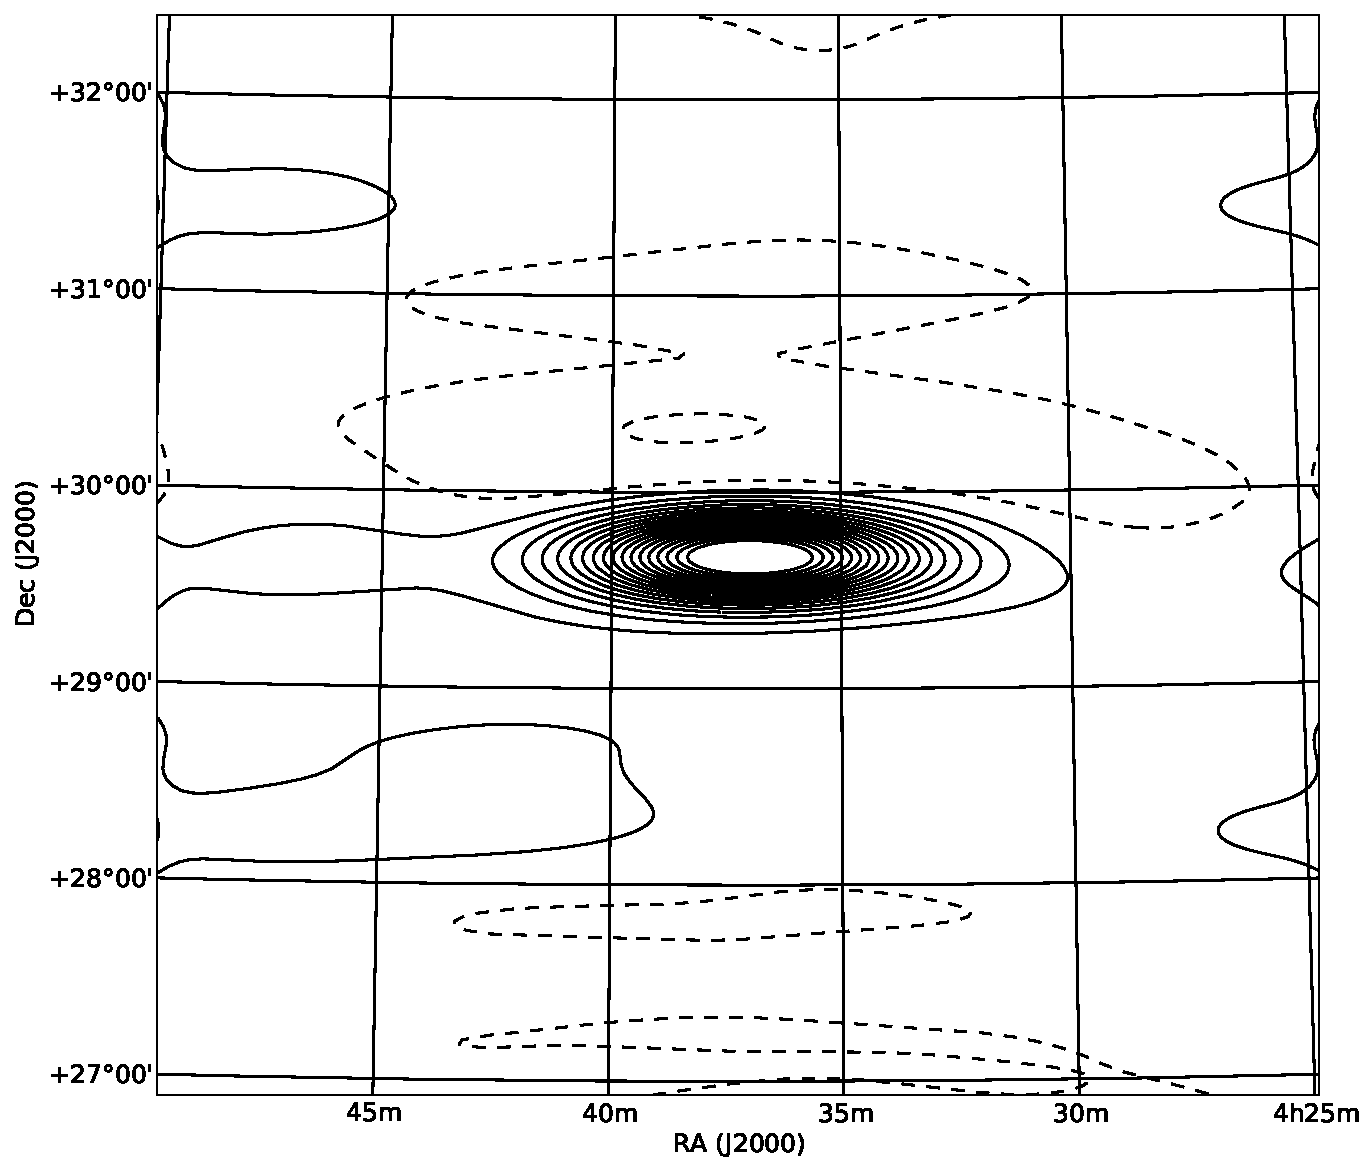
\includegraphics[scale=0.3]{{graphics/3c123/corr.2455996.19182.123.s.ms.CORRECTED_DATA.channel.1ch.restored}.pdf}
    \label{fig:fx_3c123_dirty}
    }
    \hspace{10pt}
    \subfloat[]{
    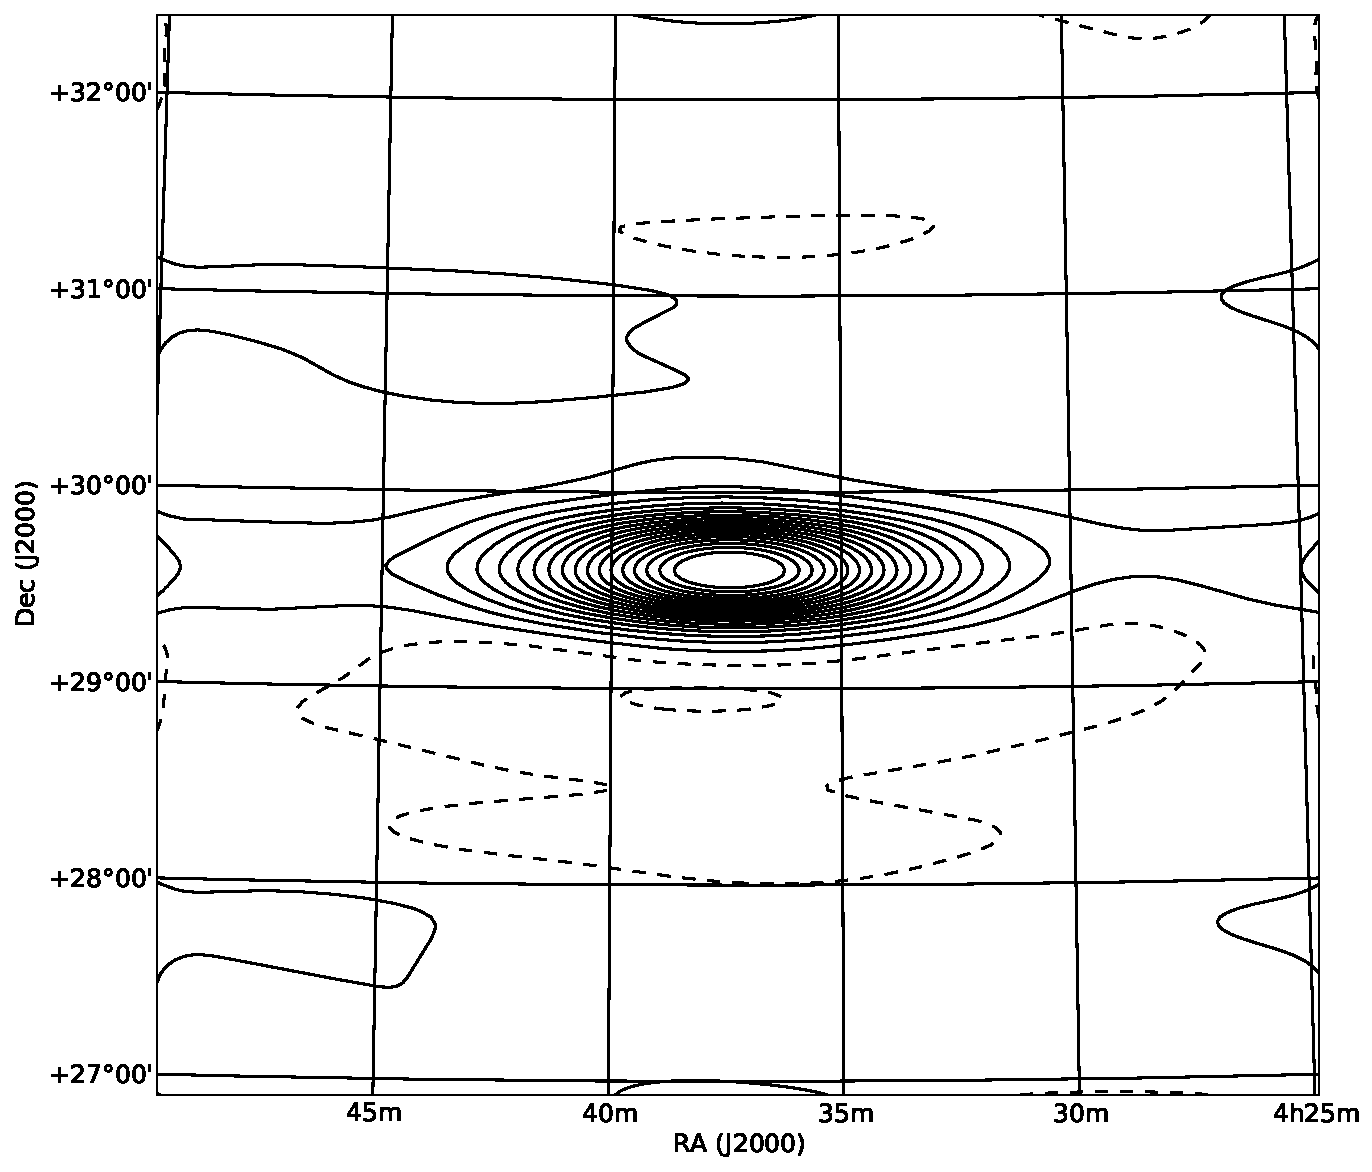
\includegraphics[scale=0.3]{{graphics/3c123/img.2455996.17741.123.s.ms.CORRECTED_DATA.channel.1ch.restored}.pdf}
    %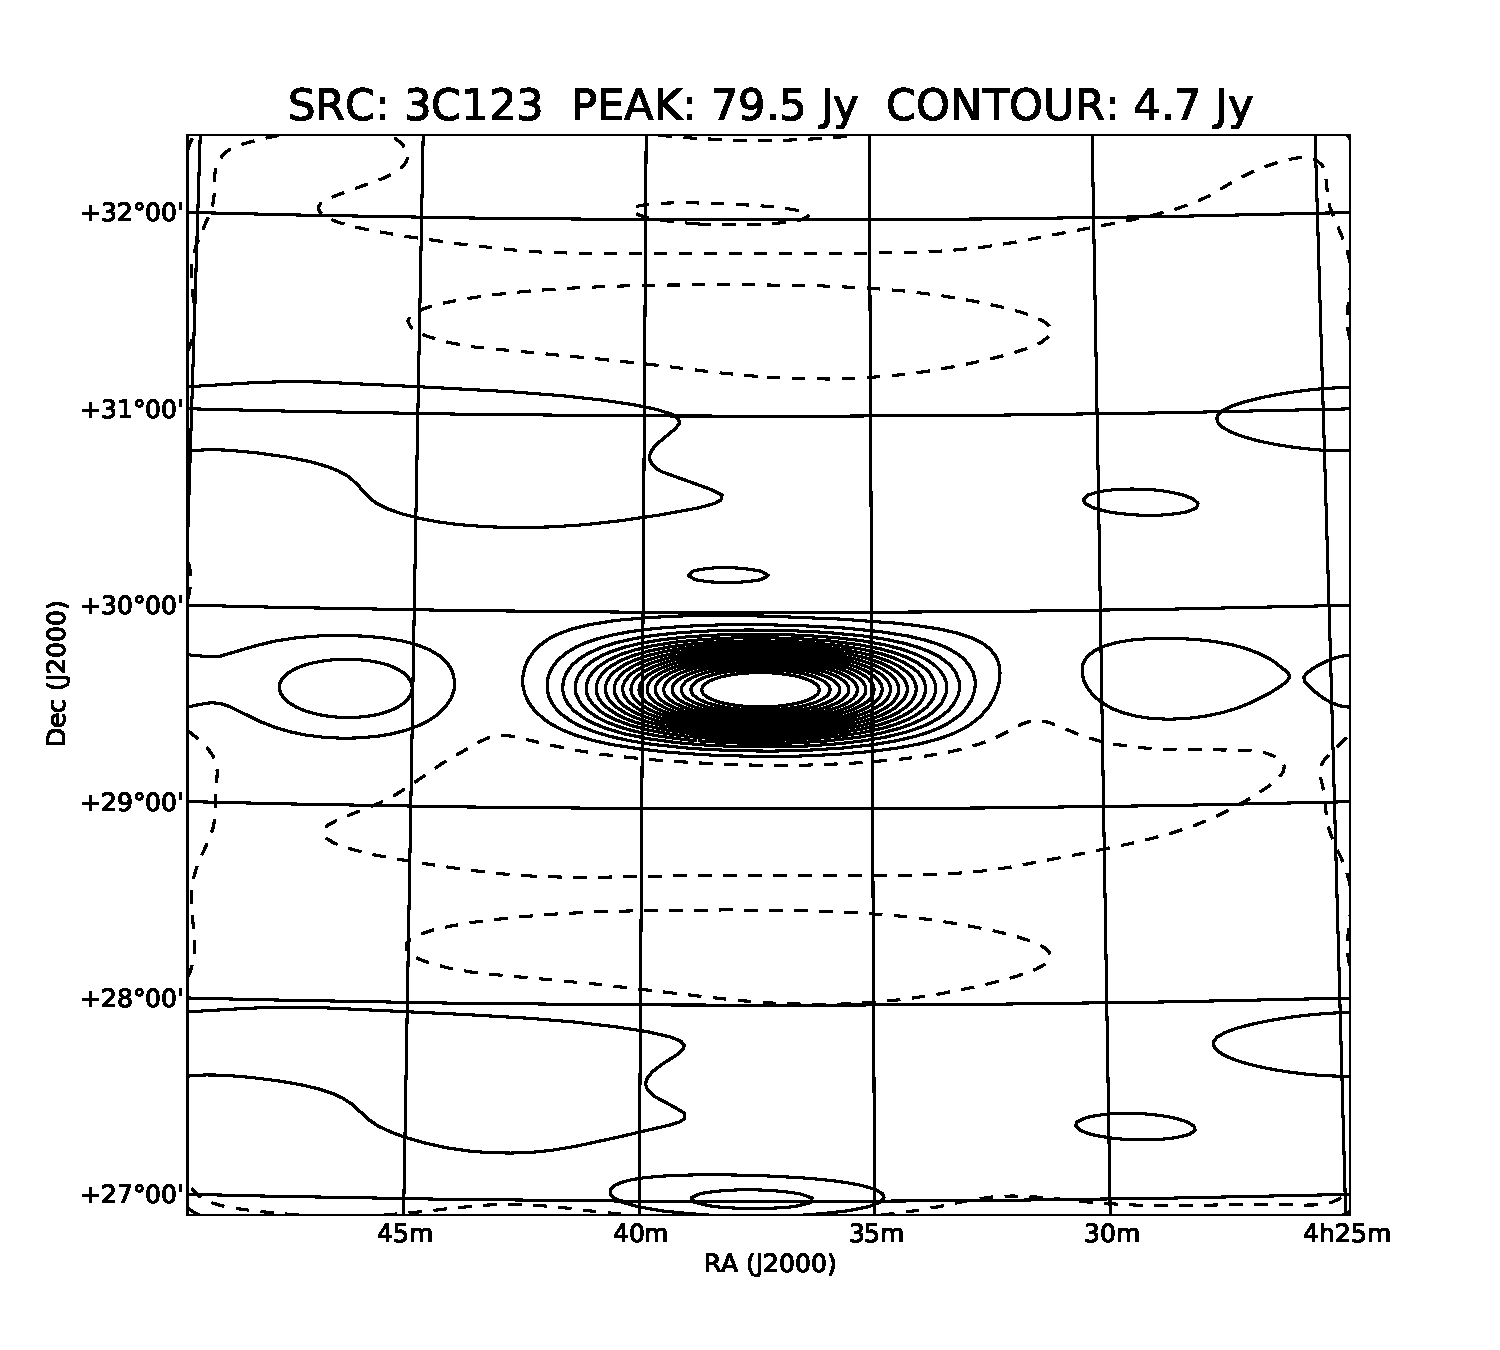
\includegraphics[scale=0.3]{{graphics/3c123/img.2455996.17741.123.s.ms.DATA.channel.1ch}.pdf}
    \label{fig:sfft_3c123_dirty}
    }

    \caption{Cleaned images formed from simultaneous observation of various sources with the FX correlator and spatial FFT imager.
    The left column is from FX correlator data, the right column is spatial FFT data.
    Sources are 3c10 (fig. \ref{fig:fx_3c10_dirty},\ref{fig:sfft_3c10_dirty}), 3c48 (fig. \ref{fig:fx_3c48_dirty},\ref{fig:sfft_3c48_dirty}), 3c123 (fig. \ref{fig:fx_3c123_dirty},\ref{fig:sfft_3c123_dirty}).
    The FX correlator and spatial FFT images have comparable noise floors of about 2 Jy in all images and difference in dynamic range varying from a few percent to 10 percent depending on the source.
    }
    \label{fig:fx_sfft_set1}
\end{figure}

\begin{figure}
    \centering

    \subfloat[]{
    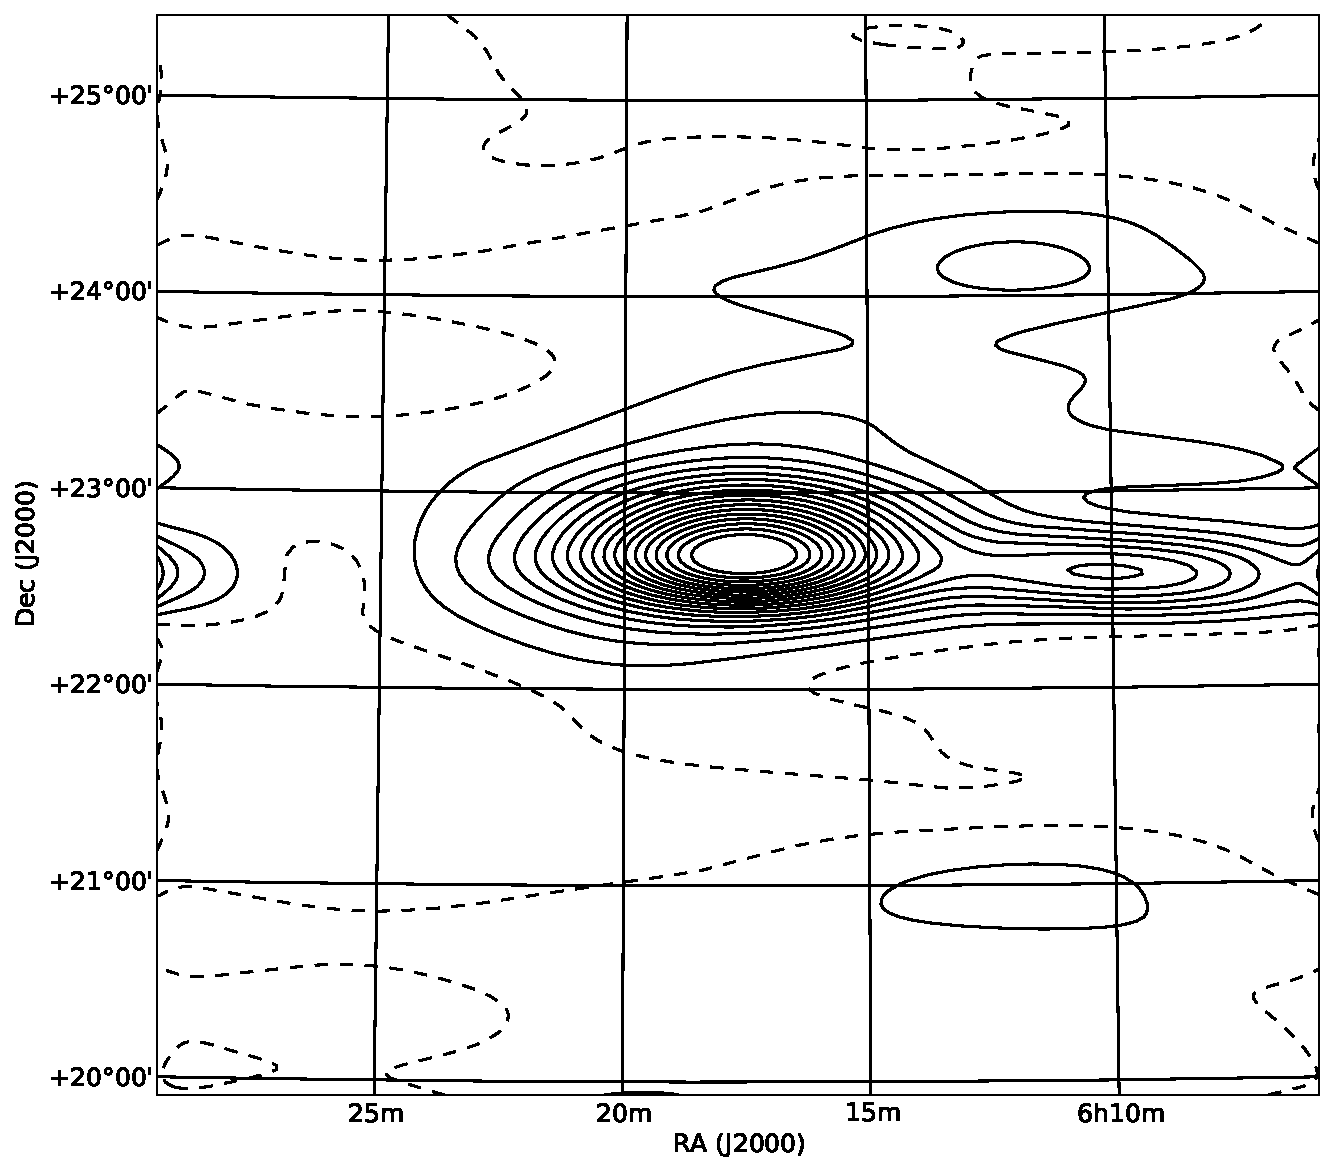
\includegraphics[scale=0.3]{{graphics/3c157/corr.2455994.26279.157.s.ms.CORRECTED_DATA.channel.1ch.restored}.pdf}
    %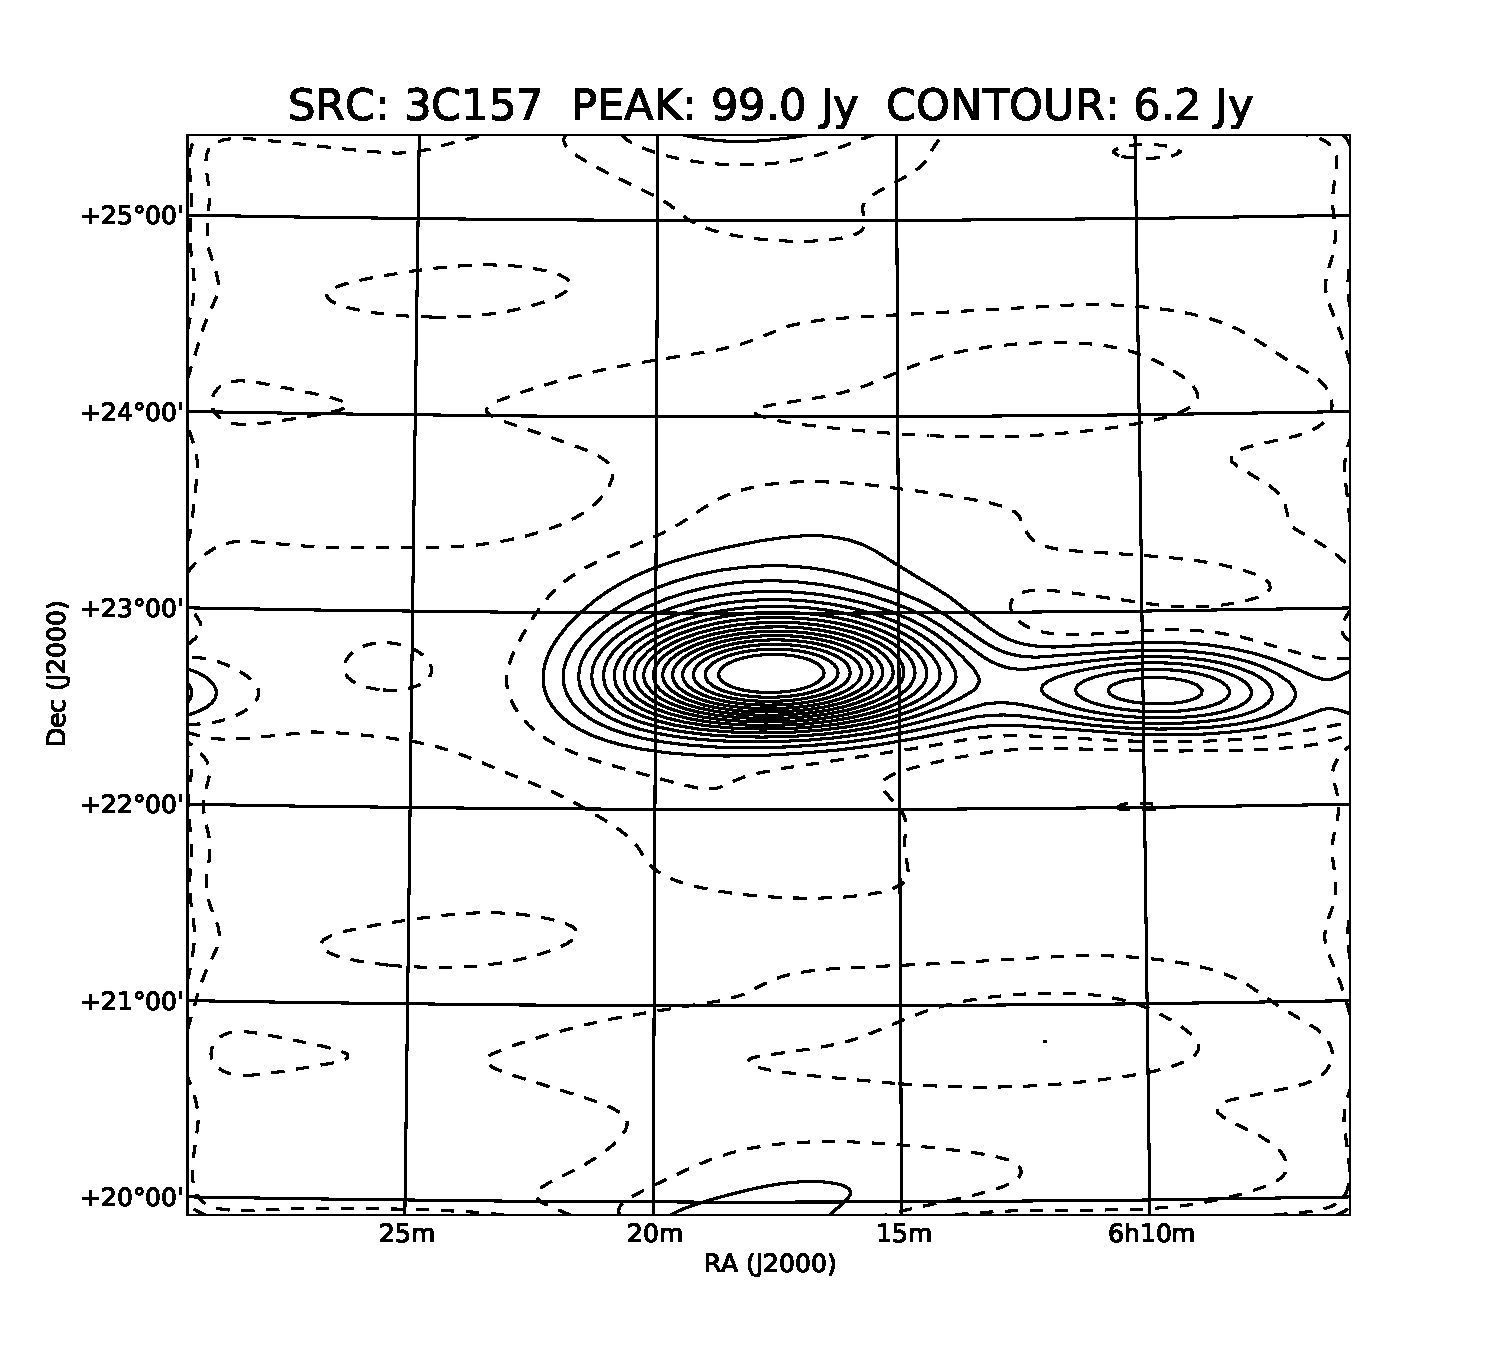
\includegraphics[scale=0.3]{{graphics/3c157/corr.2455994.26279.157.s.ms.CORRECTED_DATA.channel.1ch}.pdf}
    \label{fig:fx_3c157_dirty}
    }
    \hspace{10pt}
    \subfloat[]{
    %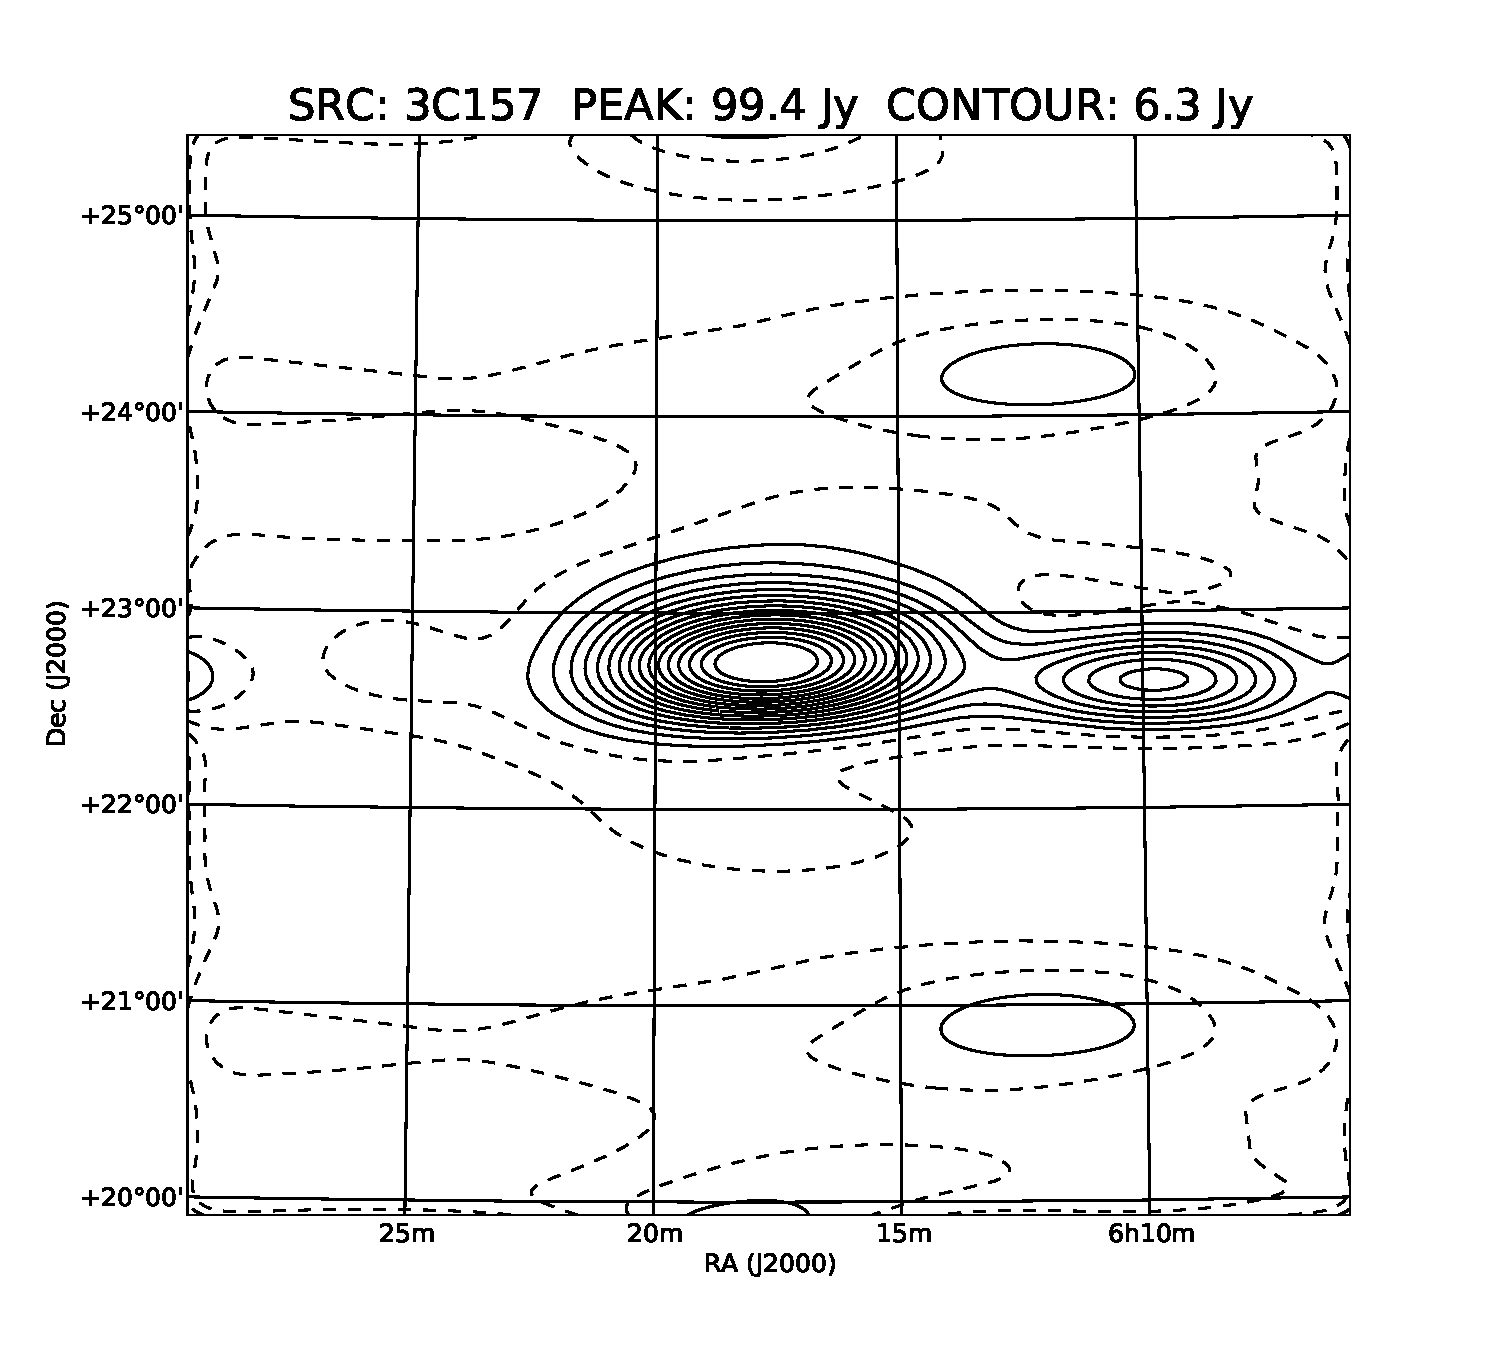
\includegraphics[scale=0.3]{{graphics/3c157/img.2455999.24137.157.s.ms.CORRECTED_DATA.channel.1ch}.pdf}
    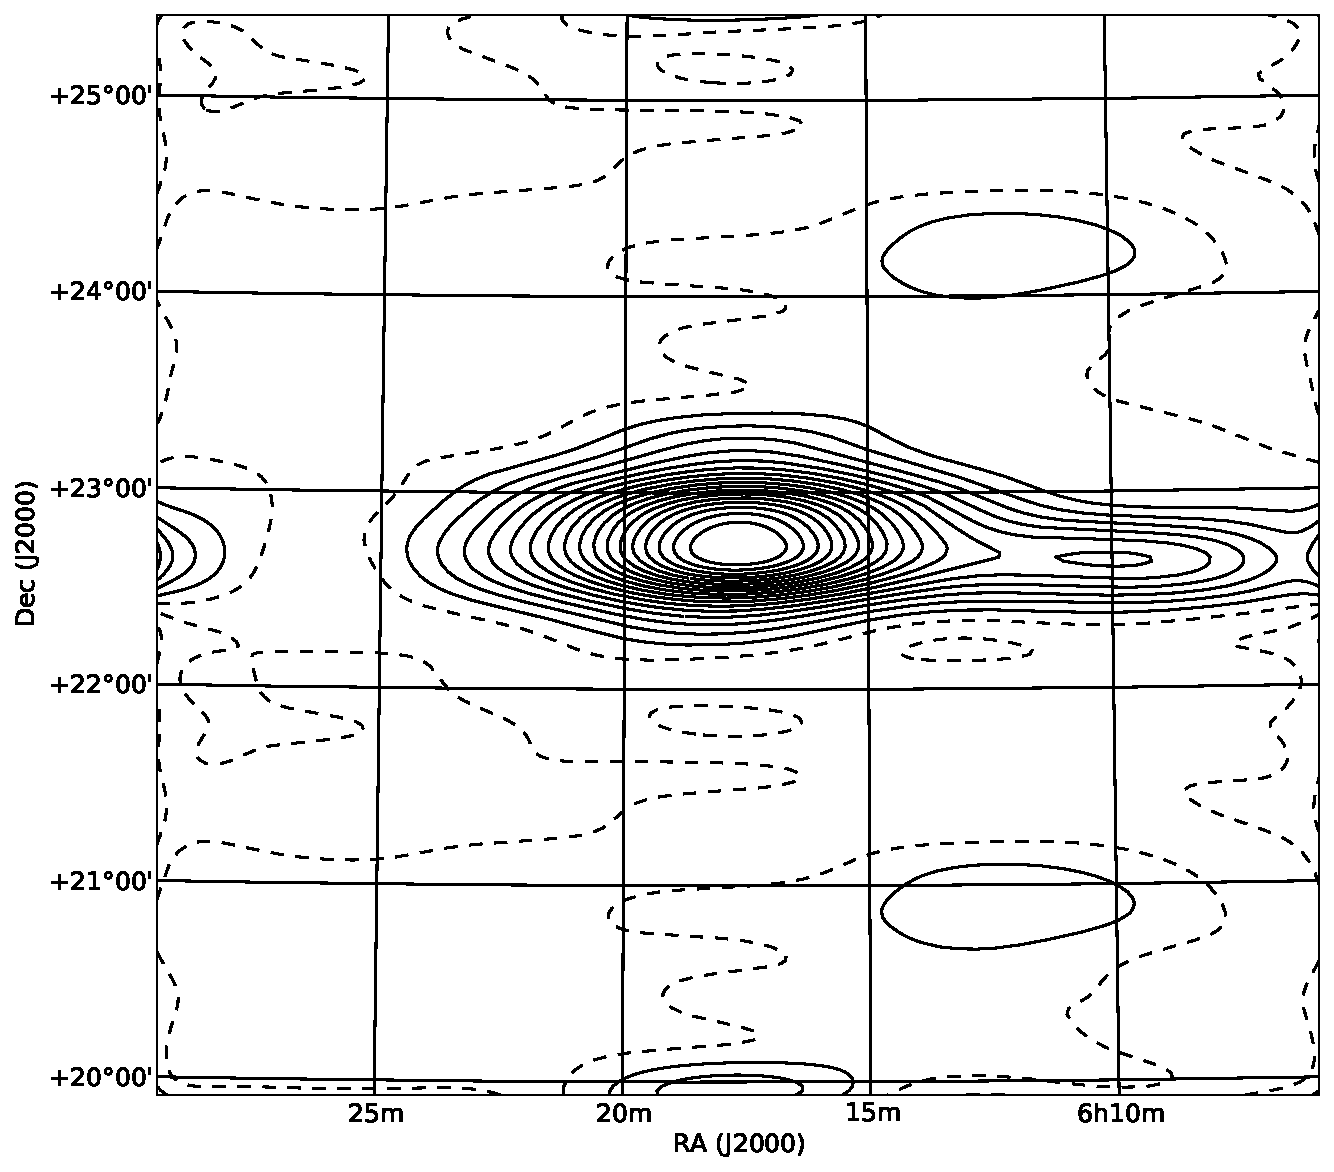
\includegraphics[scale=0.3]{{graphics/3c157/img.2455999.24137.157.s.ms.CORRECTED_DATA.channel.1ch.restored}.pdf}
    \label{fig:sfft_3c157_dirty}
    }
    \vspace{-10pt}
    
    \subfloat[]{
    %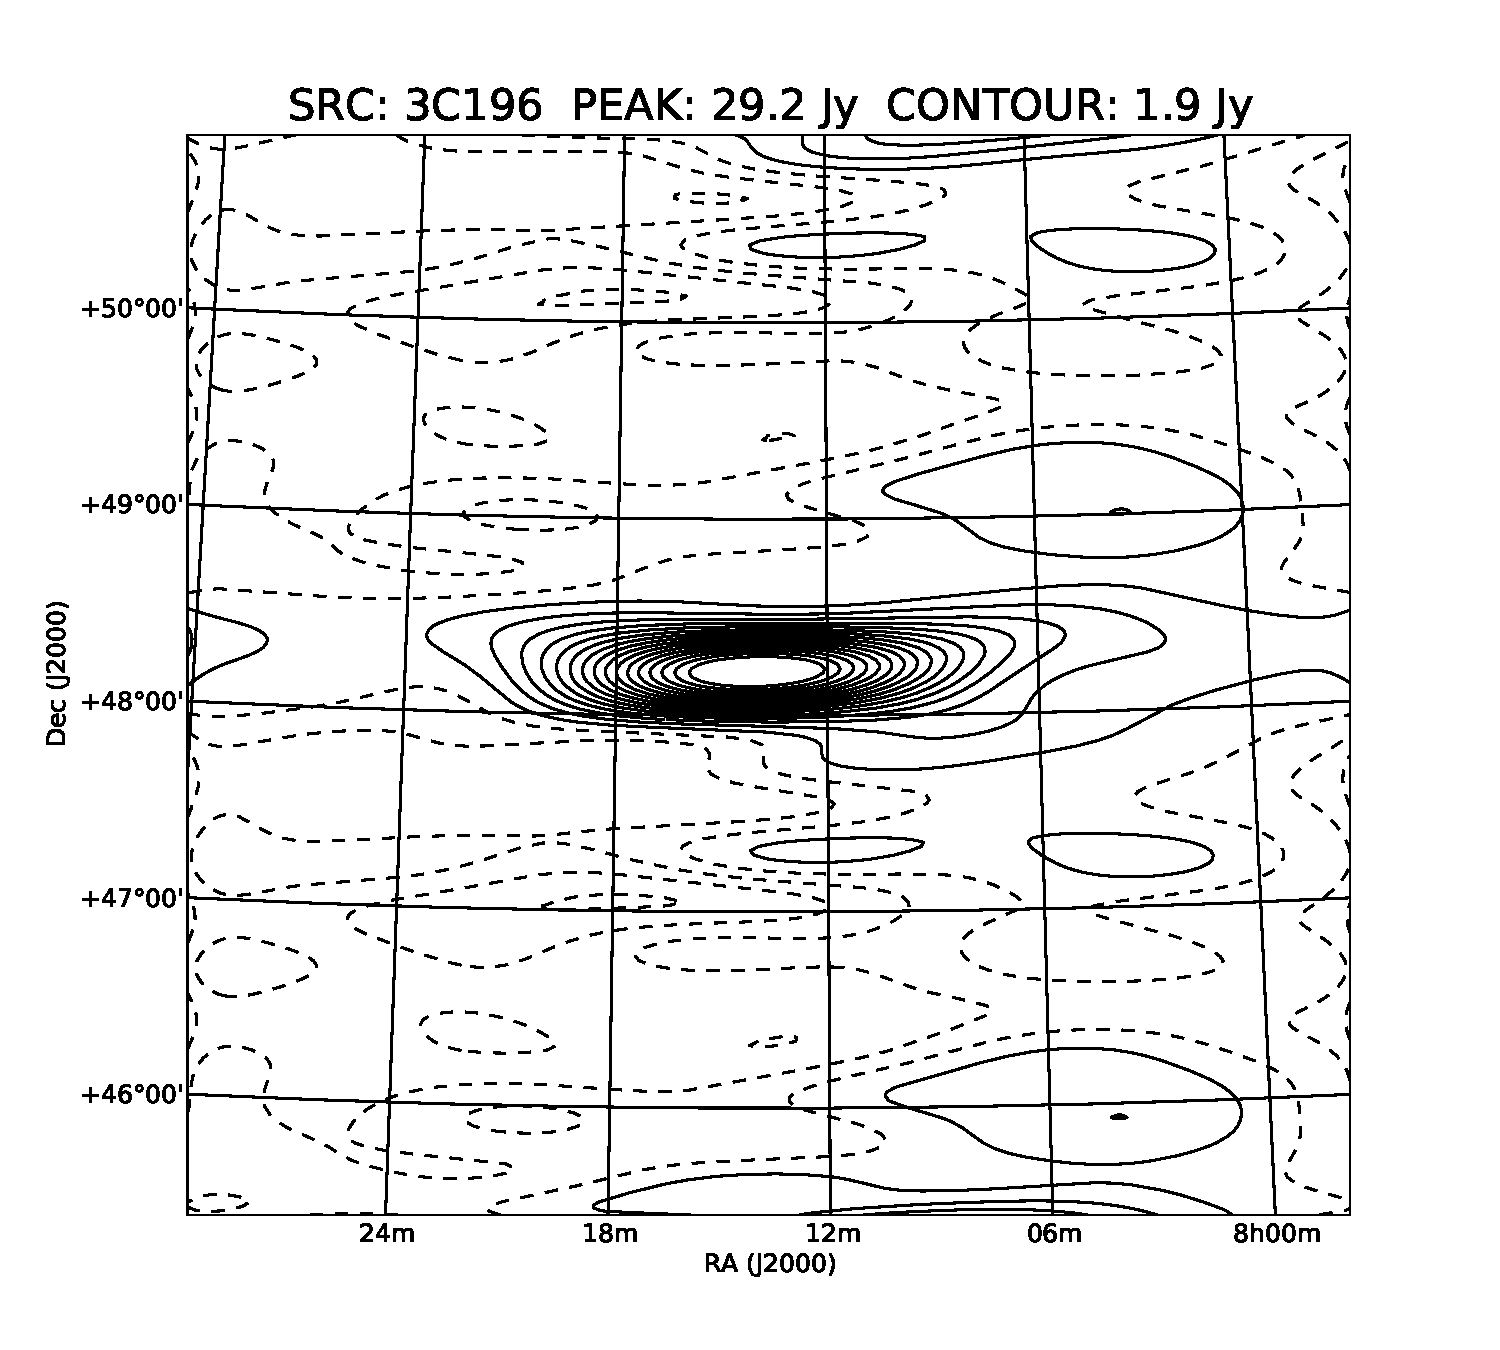
\includegraphics[scale=0.3]{{graphics/3c196/corr.2455994.34354.196.s.ms.CORRECTED_DATA.channel.1ch}.pdf}
    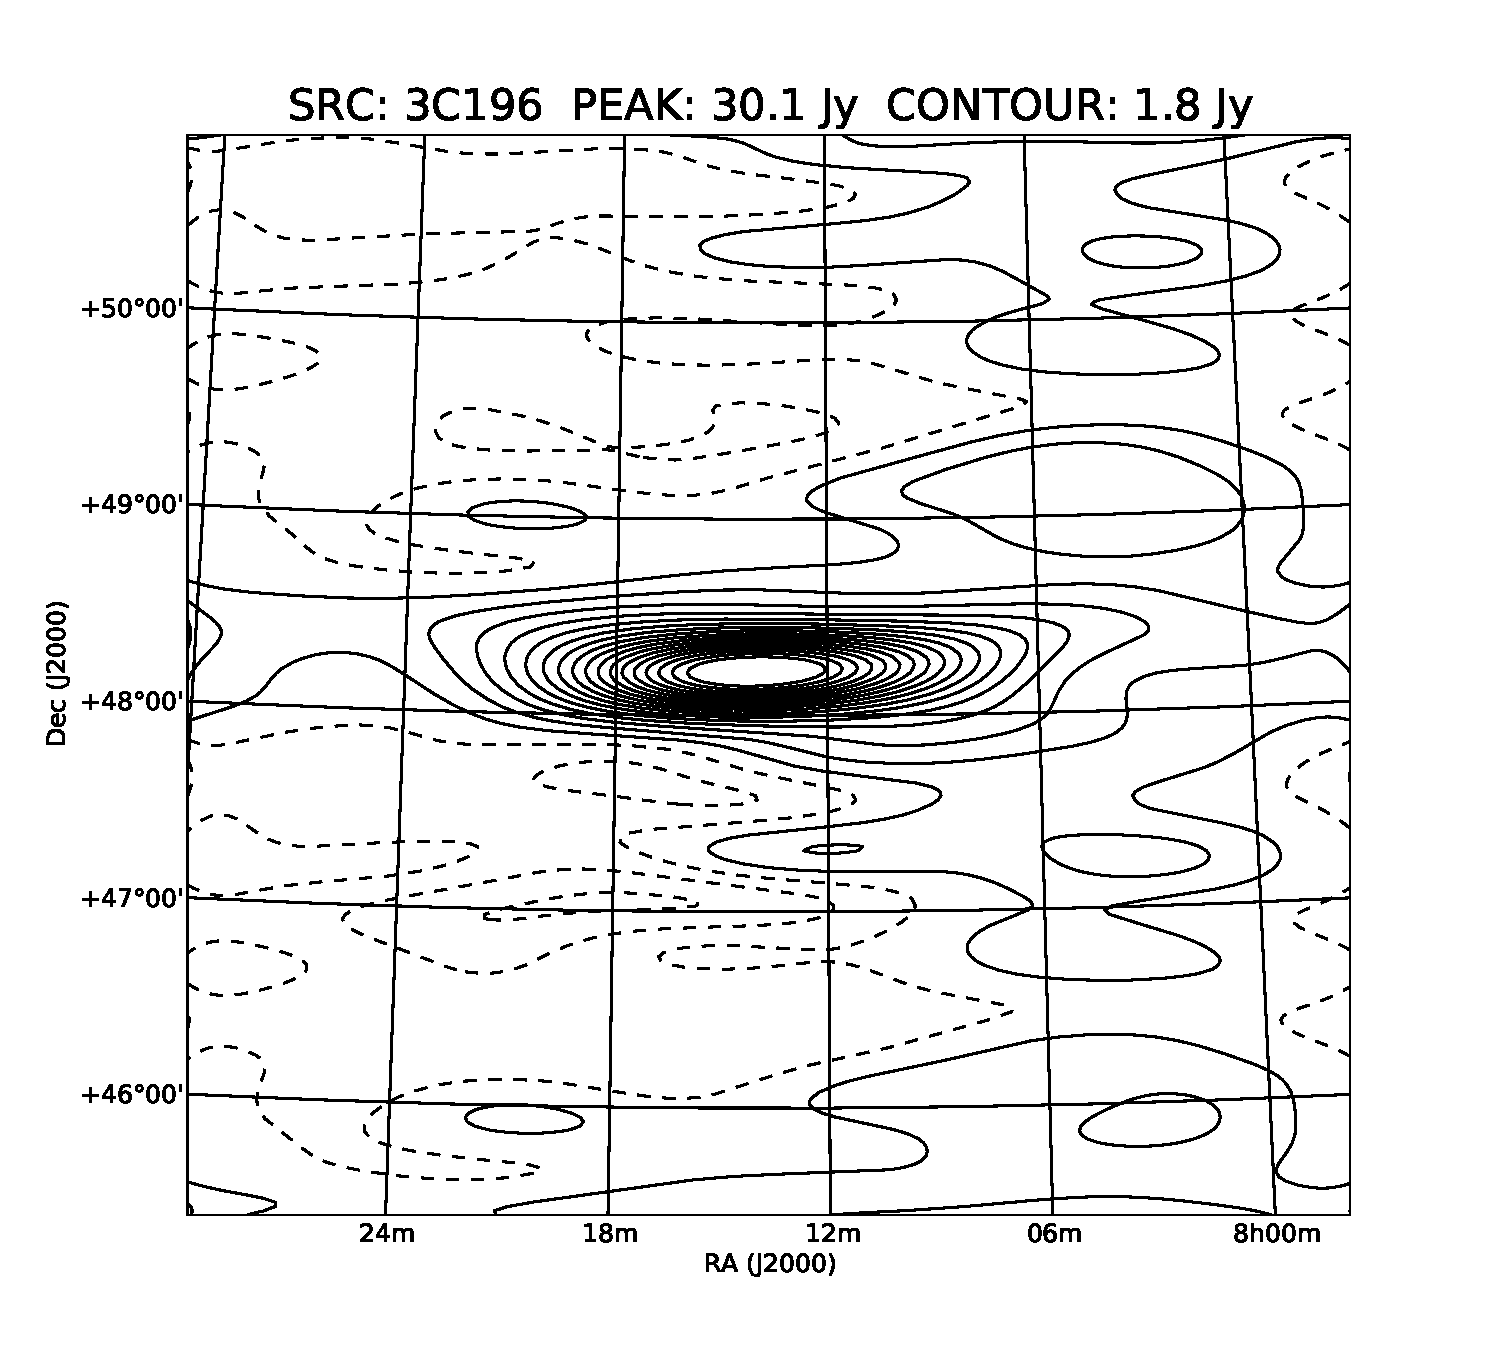
\includegraphics[scale=0.3]{{graphics/3c196/corr.2455994.34354.196.s.ms.CORRECTED_DATA.channel.1ch.restored}.pdf}
    \label{fig:fx_3c196_dirty}
    }
    \hspace{10pt}
    \subfloat[]{
    %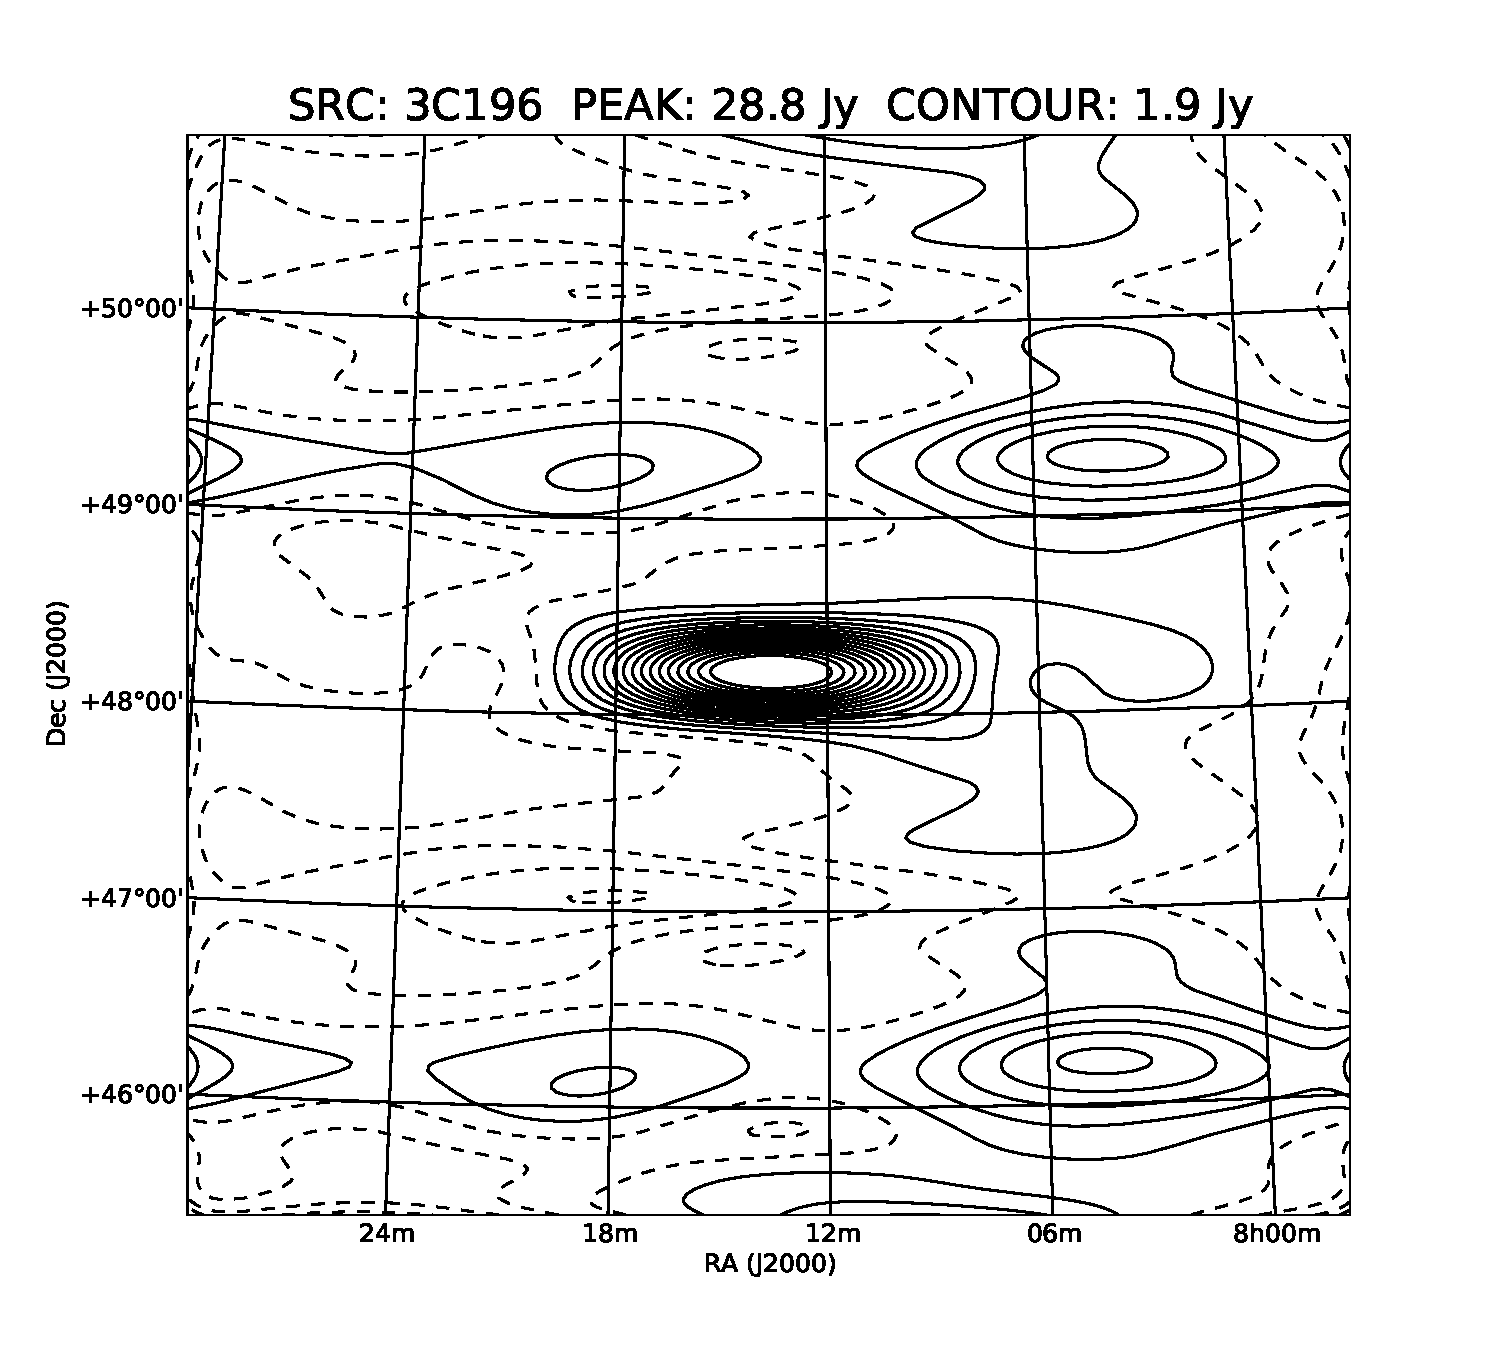
\includegraphics[scale=0.3]{{graphics/3c196/img.2455999.32370.196.s.ms.DATA.channel.1ch}.pdf}
    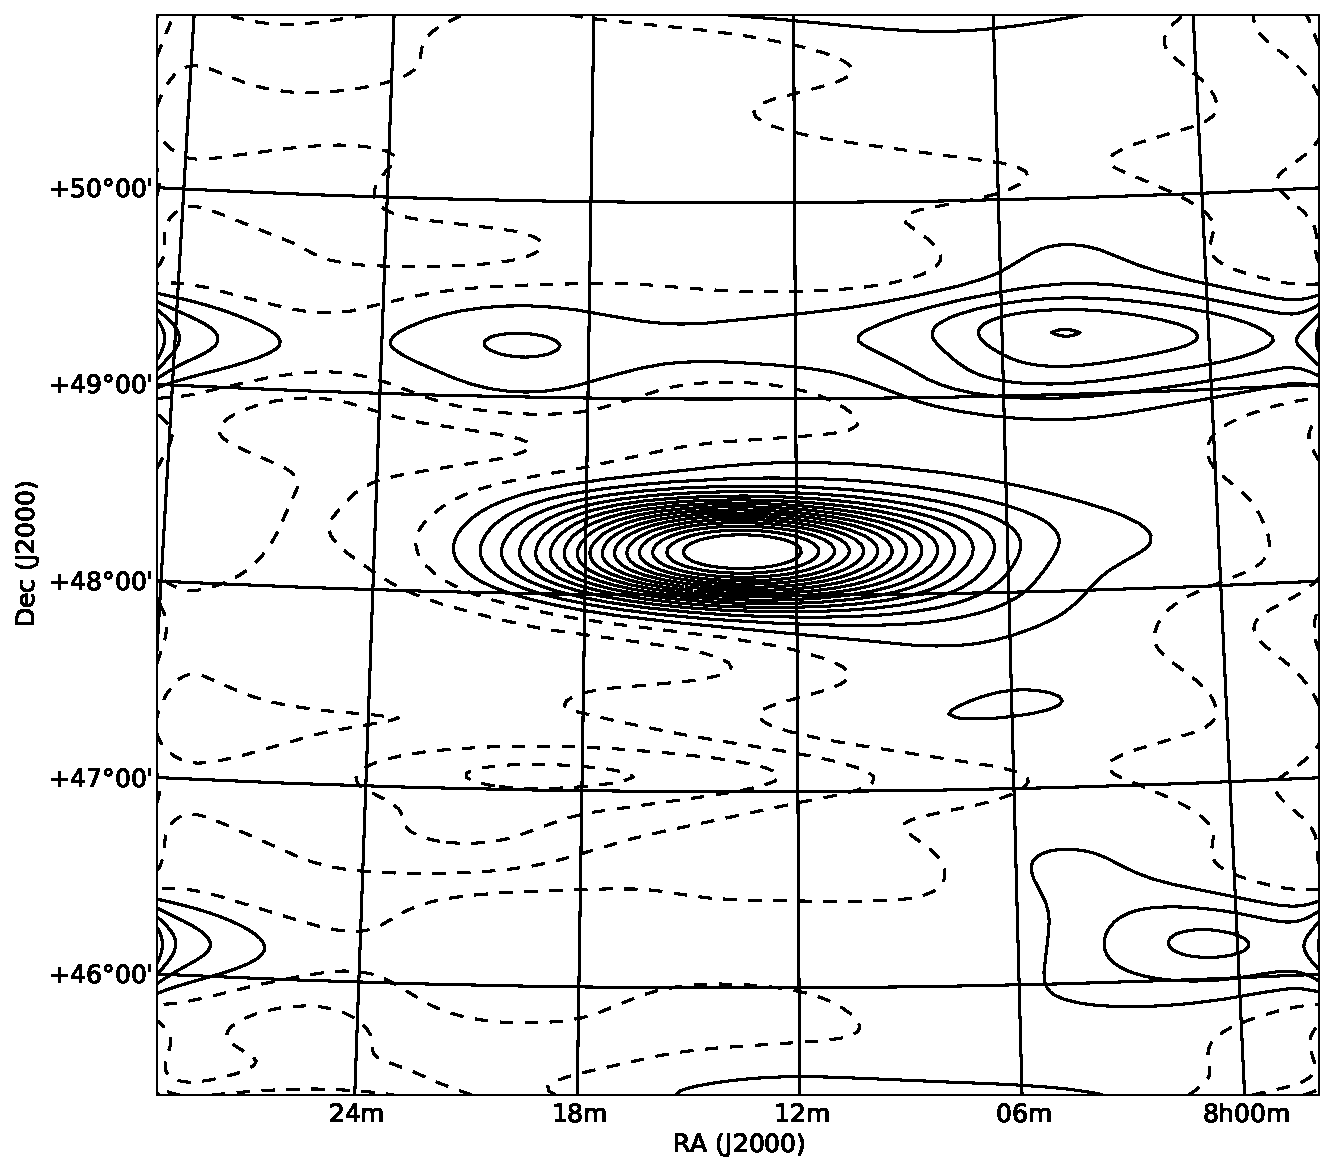
\includegraphics[scale=0.3]{{graphics/3c196/img.2455999.32370.196.s.ms.CORRECTED_DATA.channel.1ch.restored}.pdf}
    \label{fig:sfft_3c196_dirty}
    }
    \vspace{-10pt}
    
    \subfloat[]{
    %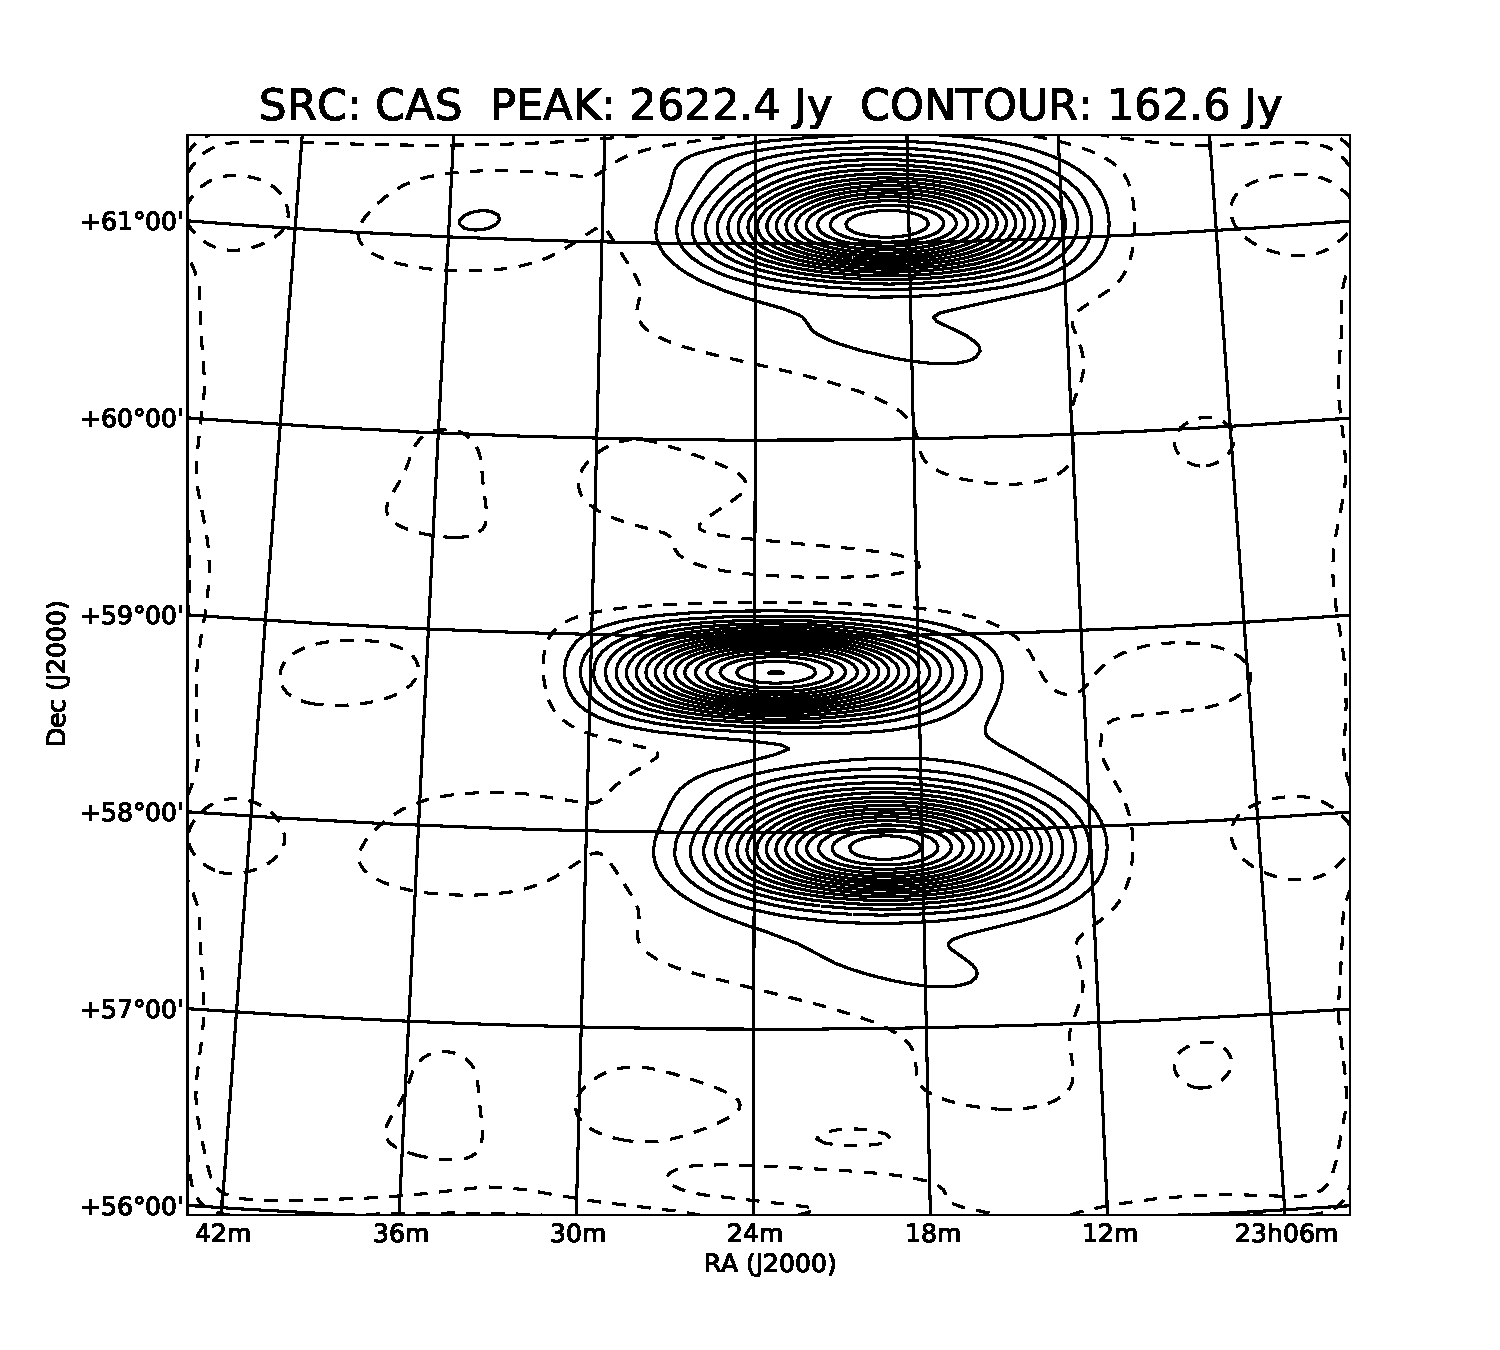
\includegraphics[scale=0.3]{{graphics/cas/corr.2455995.97200.cas.s.g.ms.CORRECTED_DATA.channel.1ch}.pdf}
    \includegraphics[scale=0.3]{{graphics/cas/corr.2455995.97200.cas.s.g.ms.CORRECTED_DATA.channel.1ch.restored}.pdf}
    \label{fig:fx_cas_sun_dirty}
    }
    \hspace{10pt}
    \subfloat[]{
    %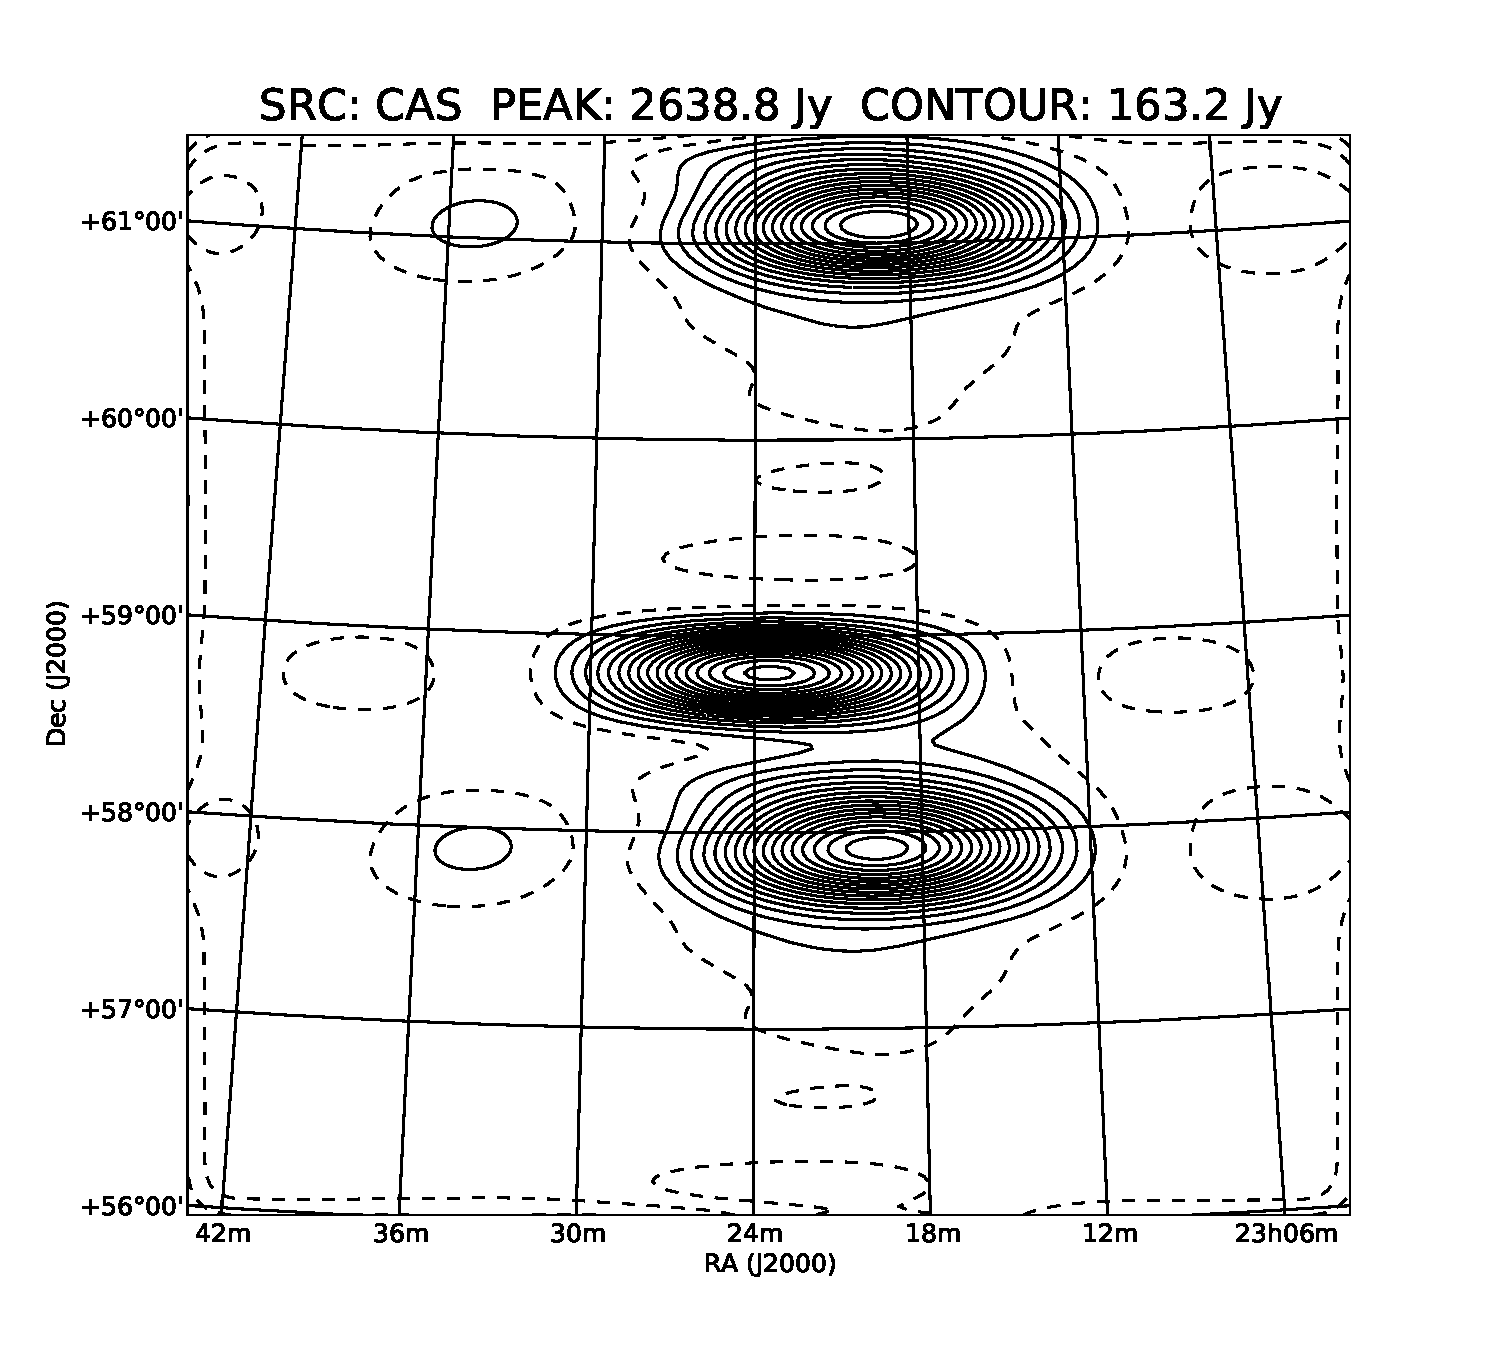
\includegraphics[scale=0.3]{{graphics/cas/img.2455995.95763.cas.s.ms.DATA.channel.1ch}.pdf}
    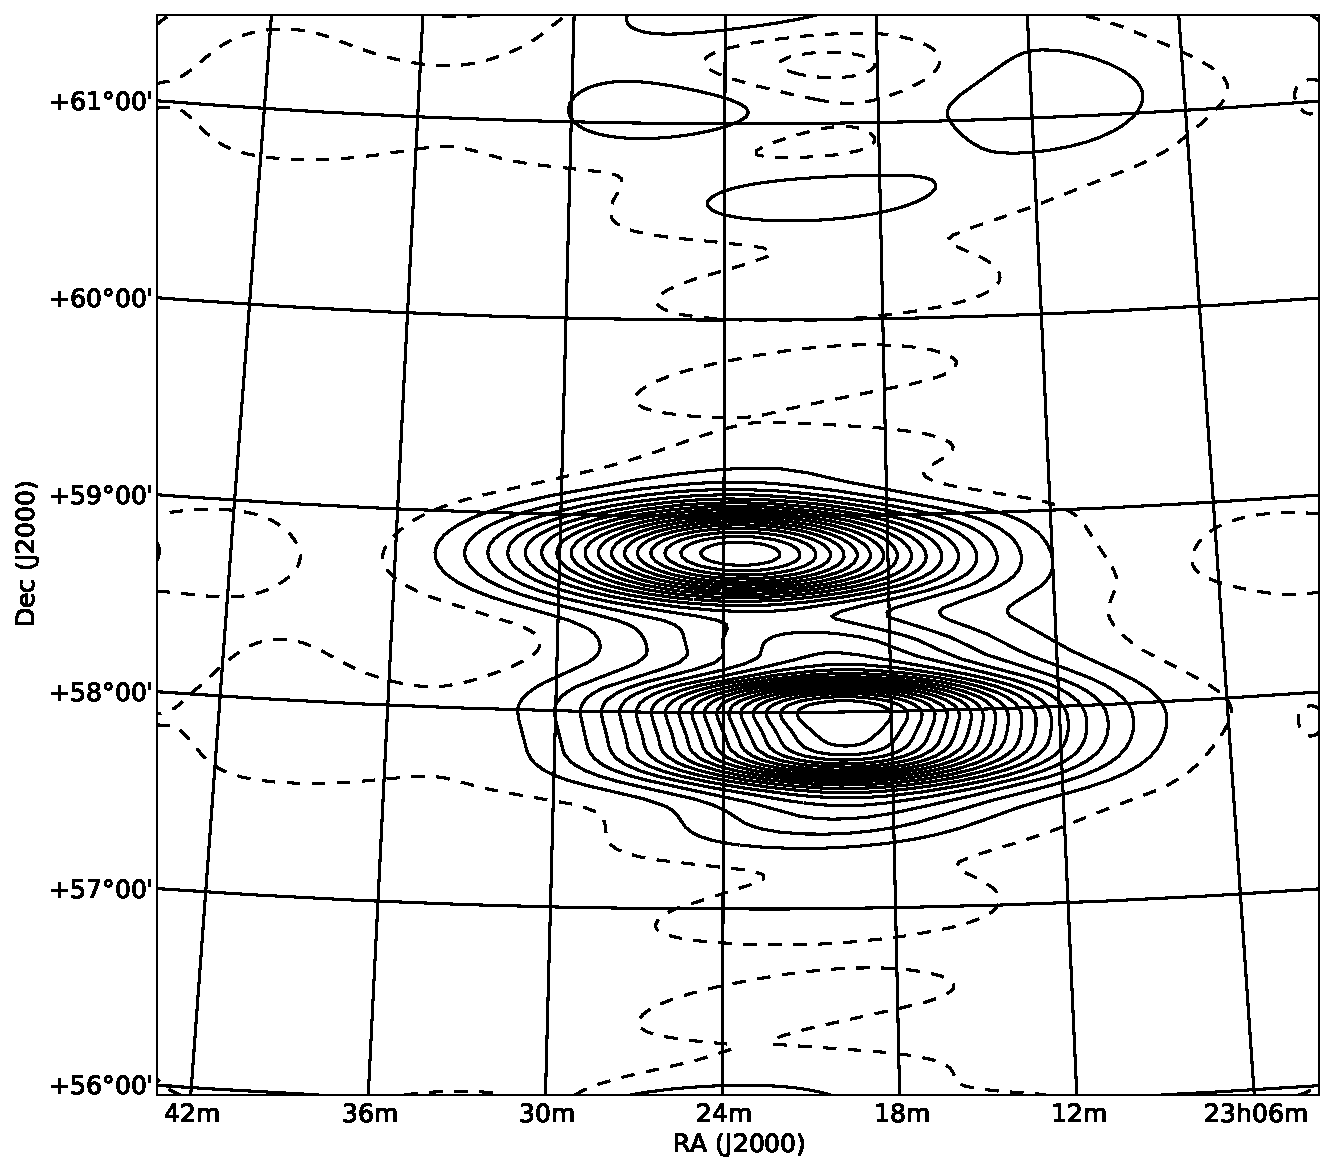
\includegraphics[scale=0.3]{{graphics/cas/img.2455995.95763.cas.s.ms.DATA.channel.1ch.restored}.pdf}
    \label{fig:sfft_cas_sun_dirty}
    }

    \caption{Cleaned images formed from simultaneous observation of various sources with the FX correlator and spatial FFT imager.
    The left column is from FX correlator data, the right column is spatial FFT data.
    Sources are 3c157 (fig. \ref{fig:fx_3c157_dirty},\ref{fig:sfft_3c157_dirty}), 3c196 (fig. \ref{fig:fx_3c196_dirty},\ref{fig:sfft_3c196_dirty}), Cassiopeia A with the sun in a sidelobe (fig. \ref{fig:fx_cas_sun_dirty},\ref{fig:sfft_cas_sun_dirty}).
    The FX correlator and spatial FFT images have comparable noise floors of about 2 Jy in all images and difference in dynamic range varying from a few percent to 10 percent depending on the source.
    }
    \label{fig:fx_sfft_set2}
\end{figure}

\bibliography{refs}{}
\bibliographystyle{mn2e}

\end{document}
